%%%%%%%%%%%%%%%%%%%%%%%%%%%%%%%%%%%%%%%%%%%%%%%%%
%
%	MSc THESIS TEMPLATE
%	developed for my master thesis at the Universitá di Torino
%
%	by Eugenio Senes (eugenio.senes@gmail.com)
%
%	released under MIT license, so share, modify and enjoy, but quoting the author !
%
%%%%%%%%%%%%%%%%%%%%%%%%%%%%%%%%%%%%%%%%%%%%%%%%%

%% DOCUMENT CLASS (alternative to book is 'report')
% Print just right page or both sides (comment the other one)
\documentclass[12pt,a4paper,openright,oneside]{book}	%%One sided
%\documentclass[12pt,a4paper,openright,twoside]{book}	%%Double sided


%% SET MARGINS OF THE PAGES
\usepackage{geometry}
\geometry{a4paper,portrait, left=35mm, right=20mm, top=35mm, bottom=30mm}

%% HEADERS AND FOOTERS
\usepackage{fancyhdr}
\pagestyle{fancy}
\fancyhf{} 			%clears default header and footer
\rhead{} 			%right head
\lhead{ \leftmark} 	%left head
\rfoot{\thepage}
%%consider using also chead, cfoot, lfoot
%coherce the plain stile to this (e.g. the first page of every chapter)
\fancypagestyle{plain}{
	\fancyhf{}
	\rfoot{\thepage}
	\renewcommand{\headrulewidth}{0pt}
	\renewcommand{\footrulewidth}{0pt}
}
%% CLEAR PAGE WITHOUT NUMBER AT THE BEGINNING OF CHAPTERS
\let\origdoublepage\cleardoublepage
\newcommand{\clearemptydoublepage}{%
  \clearpage
  {\pagestyle{empty}\origdoublepage}%
}
%% ALLOW PAGE ROTATION
\usepackage{lscape}

%% HYPERTEXT SETUP
\usepackage{hyperref}
\hypersetup{
    colorlinks,
    citecolor=black,
    filecolor=black,
    linkcolor=black,
    urlcolor=black
}
%% PDF SETTINGS
\hypersetup{
    pdfauthor={Luca Sorrentino},
    pdftitle={sorrentino_thesis},
    pdfsubject={subject},
    pdfkeywords={DRL, reinfocement learning}
}
%% FONTS AND SYMBOLS
\usepackage[utf8]{inputenc}	%%input font setting
\usepackage[T1]{fontenc} 		%%font for automatic recognition of letters with the accent
\usepackage{amsfonts}		%%fonts for the mathematical rendering of formulas
\usepackage{amssymb}
\usepackage{amsmath}
%% CHAPTERS STRUCTURE
\usepackage[italian,english]{babel} %%Set English as main language of the document
%% FIGURES
\usepackage{graphicx}
\usepackage{subfigure}		%%allow side by side figures with single caption
%% TABLES
\usepackage{multirow}		%%allow to merge rows in the tables
\usepackage{booktabs}		%%allow use of \toprule, \midrule, \bottomrule in tables
%%CAPTIONS
\usepackage{caption}
%% BIBLIOGRAPHY
\usepackage[babel]{csquotes}
%% CODE LISTINGS
\usepackage{listings}		%%allow to use code listings

%%%%%%%%%%%%%%%%%%%%%%%%%%%%%%%%%%%%% QUI

\usepackage{float}

\usepackage{amssymb}
\usepackage{amsmath}
\usepackage{amsfonts}
\usepackage{hyperref}
\usepackage{mathpazo} % Use the Palatino font by default

\usepackage[utf8]{inputenc} % this is needed for umlauts
%\usepackage[ngerman]{babel} % this is needed for umlauts
\usepackage[T1]{fontenc}    % this is needed for correct output of umlauts in pdf
\usepackage{amssymb,amsmath,amsfonts} % nice math rendering
\usepackage{braket} % needed for \Set
\usepackage{caption}
\usepackage{algpseudocode}
%\usepackage{algorithm}
\usepackage{algorithm}
\usepackage[normalem]{ulem}
%\usepackage[noend]{algpseudocode}
 \usepackage{url}
 
%%%%%%%%%%%%%%%%%%%%%%%%%%%%%%%%%%%%%%%%%%%%%%%%% FINE QUI

%% HYPENATON
\hyphenation{te-si pip-po paperino}	%manual hyphenation


%%%%%%%%%%%%%%%%%%%%%%%%%%%%%%%%%%%%%%%%%%%%%%%%%
%%%% BEGIN DOCUMENT
\begin{document}

%%%%%% HEAD  OF THE DOCUMENT
\frontmatter
%%FRONT PAGE
\begin{titlepage}
%upper part
\begin{center}
{{\Large{\textsc{Universit\`a degli studi di Torino \\}}}} \vspace{5mm} {\small{\bf Dipartimento Di Informatica\\ \vspace{3mm}
Corso di Laurea Magistrale in Informatica}}
\vspace{5mm}
\end{center}
%logo
\begin{center}

\includegraphics[scale=.3]{head/logo.png}
\end{center}
%title
\begin{center}
\vspace{5mm}
{\large{\bf Master's Degree Thesis \\}}
\vspace{5mm}
{\LARGE{\bf Overcoming the limits of DRL \\ with Model-Based approach }}
%\vspace{5mm}
%{\LARGE{\bf SECOND ROW TITLE}}
\end{center}
\vspace{20mm}
%relatore
\par
\noindent
\begin{minipage}[t]{0.47\textwidth}
{\large{\bf Supervisor:\\
Prof. Marco Aldinucci\\
Antonio Mastropietro}}
\end{minipage}
\hfill
\begin{minipage}[t]{0.47\textwidth}\raggedleft
{\large{\bf Candidate:\\
Luca Sorrentino}}
\end{minipage}
\vspace{10mm}
\begin{center}
\vspace{20mm}
{\large{\bf 
Anno Accademico 2019/2020}}
\end{center}

\end{titlepage}
%\begin{titlepage}
%upper part
\begin{center}
{{\Large{\textsc{Universit\`a degli studi di Torino \\}}}} \vspace{5mm} {\small{\bf SCUOLA DI SCIENZE DELLA NATURA\\ \vspace{3mm}
Corso di Laurea Magistrale in Fisica}}
\vspace{5mm}
\end{center}
%logo
\begin{center}

\includegraphics[scale=.3]{head/logo.png}
\end{center}
%title
\begin{center}
\vspace{5mm}
{\large{\bf Tesi di Laurea Magistrale\\}}
\vspace{5mm}
{\LARGE{\bf THE FANCY TITLE\\ OF MY FANCY THESIS\\}}
%\vspace{5mm}
%{\LARGE{\bf SECOND ROW TITLE}}
\end{center}
\vspace{20mm}
%reatori e candidato
\vspace{11mm}
\par
\noindent
\begin{minipage}[t]{0.47\textwidth}
{\large{\bf Relatore:\\
Prof. Zio Paperone}}\\
\vspace{4mm}
\\
{\large{\bf Correlatore:\\
Dr. Pico de Paperis (PAP) }}
\vspace{8mm}
{\large{\bf \\ Controrelatore:\\
Prof.ssa Nonna Papera}}
\end{minipage}
\hfill
\begin{minipage}[t]{0.47\textwidth}\raggedleft
\vspace{16mm}
{\large{\bf Candidato:\\
Paperoga}}
\end{minipage}
\vspace{9mm}
\begin{center}
{\large{\bf 
Anno Accademico 20xx/20xx}}
\end{center}

\end{titlepage}

\newpage
\thispagestyle{plain} % empty
\mbox{}

\clearemptydoublepage
%%ABSTRACT
\chapter*{Abstract}

Reinforcement Learning (RL) is a subfield of Machine Learning where an agent learns to solve a task by interacting with the environment by trial and error without explicit knowledge. The agent receives a reward signal as feedback for every action it takes, and it learns to prefer those accompanied by a positive reward over those accompanied by a negative reward. 
This simple formulation allows the agent to directly choose the right actions from sensory observations, e.g. high dimensional inputs like camera frames, and to solve many complex tasks, like playing video-games or controlling robots.  \\ 
The standard formulation exposed before is called Model-Free Reinforcement Learning because it does not require the agent to predict explicitly the environment dynamics, thus it can be viewed as a black-box approach. However, it requires a tremendous amount of experience and the lack of sample efficiency limits the usefulness of these algorithms in practice. 
One possible solution to overcome this problem is to combine the Reinforcement Learning framework with planning algorithms. 
This approach is called Model-Based RL.
Instead of directly mapping observations to actions, Model-based RL allows the agent to plan explicitly the sequence of actions to be taken by observing the environment dynamics predicted by an environment model. \\
In recent years RL has been combined with Deep Learning algorithms to obtain outstanding results and reach superhuman performance in complex tasks. This combination of Reinforcement Learning and Deep Learning has been called Deep Reinforcement Learning (DRL).
In this thesis, one of the state-of-the-art Model-Based DRL algorithms called PlaNet is deeply investigated and compared with the model-free DRL algorithm called Deep Deterministic Policy Gradient (DDPG). 
All the experiments are based on Deepmind Control Suite that is a set of continuous control tasks that are built for benchmarking reinforcement learning agents. Both the algorithms examined were tested on a subset of four environments.
The main strengths and weaknesses of both approaches are highlighted in order to show if and how much a Model-Based RL can overcome the limits of Model-Free RL.\\

I declare that the material submitted for assessment is my own work except where credit is explicitly given to others by citation or acknowledgement.

\chapter*{Italian abstract}

Il Reinforcement Learning (RL) è una tecnica di Machine Learning in cui vi è un agente che impara a risolvere un task interagendo col l’ambiente in cui si trova e di cui non ha nessuna conoscenza procedendo con un approccio trial and error. L’agente riceve un segnale di feedback chiamato reward per ogni azione che compie e impara a favorire quelle azioni accompagnate da un reward positivo a discapito di quelle accompagnate da un reward negativo. 
Questa semplice formulazione permette all’agente di prevedere le migliori azioni a partire dai sensori di input, come ad esempio i frame della camera, e di risolvere quindi molti task complessi, come giocare a videogiochi o controllare robot.
La formulazione standard espressa finora viene definita Model-Free Reinforcement Learning perchè non richiede all'agente di costruirsi un modello dell'environment e di prevederne esplicitamente le dinamiche.
Purtroppo, questo approccio diretto richiede un numero tremendamente elevato di esperienza e questo scarso livello di sample-efficiency limita l’utilità di questi algoritmi nell’uso pratico.
Una possibile soluzione per superare questo problema è quella di combinare il Reinforcement Learning con algoritmi di planning.
Questo approccio è chiamato Model-Based DRL.
Invece di creare un mapping diretto tra osservazioni e azioni, il MBDRL permette all'agente di pianificare in modo esplicito la sequenza di azioni da intraprendere in base alle previsioni sugli sviluppi dell’ environment.

Negli ultimi anni il RL è stato combinato con algoritmi di Deep Learning ottenendo cosi risultati eccezionali arrivando a superare umani esperti anche in task complessi.
Questa combinazione di RL e DL prende il nome di Deep Reinforcement Learning (DRL).
In questa tesi, uno degli più recenti algoritmi di Model-Based DRL chiamato PlaNet viene esplorato e comparato con un algoritmo di Model-Free DRL chiamato Deep Deterministic Policy Gradient.
Tutti gli esperimenti sono basati sulla Deepmind Control Suite, un set di task creati per effettuare benchmark di agenti addestrati tramite DRL. Entrambi gli algoritmi presi in esame sono stati testati su quattro environments.
I maggiori punti di forza e di debolezza dei due approcci vengono messi in luce per mostrare se e quanto l’approccio Model-Based sia in grado di superare i limiti del Model-Free DRL.\\

“Dichiaro che il sottoscritto nonché autore del documento è il responsabile del suo contenuto, e per le parti tratte da altri lavori, queste vengono espressamentedichiarate citando le fonti”


\clearemptydoublepage
%%DEDICATION (the initial quote)
\thispagestyle{empty}
\begin{flushright}

\vspace*{60mm}

"When I started working on neural network models in the 1970s,\\
people in artificial intelligence kept telling me that Minsky and Papert\\
have proved that these models were no good.”\\
\vspace{4mm}
\hfill Geoffrey Hinton\\

\vspace*{40mm}

“I wanted to just prove everybody wrong.”\\
\vspace{4mm}
\hfill Marshall Mathers\\


%\vspace*{40mm}
%“Dichiaro che il sottoscritto nonché autore del
%documento è il responsabile del suo contenuto, e per le
%parti tratte da altri lavori, queste vengono espressamente %dichiarate citando le fonti”

\end{flushright}
\clearemptydoublepage
% Acknowledgments
\chapter*{Acknowledgements}
\thispagestyle{empty}

Questo lavoro segna una tappa importante di un percorso iniziato già qualche anno fa quando, implementando A* vidi per la prima volta un software che portava a termine un compito senza richiedere una esplicita soluzione da programmare. A* aveva però molti limiti, uno in particolare era la richiesta di un umano che si specializzasse abbastanza da riuscire a trovare un'euristica per quel problema.  Da quel momento nacque in me la volontà di creare un agente che fosse il più autonomo possibile, limitando in maniere sempre maggiore l'ingerenza umana. Ben presto iniziai a concentrare le mie energie sull'apprendimento per rinforzo, per permettere alla IA di imparare direttamente dalla propria esperienza, e sulle reti neurali per aumentare la potenza espressiva della mente dell'agente (percezione visiva, memoria, capacità rappresentativa).
\\
\newline
Quando ho iniziato questo percorso ero convinto che avrei saltato questa pagina, visto che ero circondato da gente scettica che non mi era di aiuto e anzi frenava il mio entusiasmo. Dopo poco fortunatamente trovai una via di fuga attraverso il web. Per cui il mio primo ringraziamento va a chiunque utilizzi questo potente mezzo per trasmettere conoscenza. In particolar modo vorrei ringraziare: Salman Khan, Andrew Ng, David Silver, Sergey Levine.
\\
\newline
Dopo un primo anno di studio autonomo e parallelo rispetto a quello universitario, avevo maturato una piccola conscenza di base che ho poi avuto modo di ampliare durante il mio percorso in Addfor. Il mio secondo ringraziamento va quindi a loro per avermi accolto e per aver creduto ed investito in me, fornendomi l'attrezzatura tecnica necessaria ed il supporto, sia sul piano tecnico che su quello umano. Un ringraziamento particolare ad Antonio, Sonia ed Enrico.
\\
\newline
Infine, il mio terzo ringraziamento va alla mia famiglia per il supporto, ai miei colleghi per avermi accompagnato in questo percorso ed ai miei amici (lontani e vicini) per avermi incoraggiato quando le aspettative si facevano vertiginose, per aver sopportato la mia assenza quando le scadenze si avvicinavano e per avermi sostenuto e consigliato quando gli esperimenti fallivano. 
Un ringraziamento particolare va a Erica per essere riuscita a farmi ritrovare la serenità persa in questi ultimi anni.

\clearpage
\clearemptydoublepage

%%INDEXES
%summary
\tableofcontents
\clearemptydoublepage
\newpage
\thispagestyle{plain} % empty
\mbox{}


%%%%%% BODY OF THE DOCUMENT
\mainmatter
%%INTRODUCTION
% Chapter 1


\chapter{Introduction} % Main chapter title

\label{Chapter1} % For referencing the chapter elsewhere, use \ref{Chapter1} 
The idea of \textbf{Reinforcement Learning} (RL) has been known since \textbf{Turing}'s time.
He talked about it in his article "Computing machinery and intelligence":
"We normally associate punishments and rewards with the teaching process. 
Some simple child machines can be constructed or programmed on this sort of principle. 
The machine has to be so constructed that events that shortly preceded the occurrence of a punishment signal are unlikely to be repeated. In contrast, a reward signal increased the probability of repetition of the events, which led up to it.\cite{turing2009computing}"
This idea is now called reinforcement learning and consists of training an agent to achieve a goal by interacting directly in an environment without prior knowledge. The agent receives positive or negative feedback for each action it takes and tries to accumulate positive rewards.
From that time to our day, a lot of progress has been achieved.
In recent years RL has been combined with Deep Learning algorithms to obtain outstanding results and reach superhuman performance in complex tasks, for example learning to play Go from scratch \cite{silver2016mastering} or flying an acrobatic model helicopter \cite{abbeel2007application}.\\

Unfortunately, in order to reach some impressive results, these methods require a prohibitive amount of samples.
For example, in 2019, Open AI released OpenAI Five: the first AI able to beat the world champions in an e-sports game called Dota 2 \cite{berner2019dota}. 
Despite the incredible result, the training cost was tremendous, the authors report that the OpenAI Five has experienced an average of 250 years of simulated experience per day. This is the reason why the main exciting results are obtained  with agents that act in a virtual environment.
Sometimes, these algorithms are also used to train a real world agent \cite{andrychowicz2020learning}, but the training is mostly performed into a simulator.
Build a simulator each time we need to train an agent for a task can be too expensive,for example think about a robot that learns to run, and it is an open research problem how to transfer the learned policy reliably to the real world.
At the same time, the idea of performing millions of experiments with a physical robot in a reasonable amount of time and without hardware wear and tear  is unrealistic.
Alan Turing had already foreseen this problem, and in his article, he says: "The use of punishments and rewards can at best be a part of the teaching process... By the time a child has learned to repeat 'Casabianca' he would probably feel very sore indeed".
One of the most promising solutions to improve the sample efficiency is the Model-Based approach that combines the power of supervised learning, the reinforcement learning framework, and the planning algorithms. 
The key idea is to learn the environment's transition model to allow the agent to simulate interactions instead of acting directly without any knowledge.
There are several approaches to learn predictive models of the dynamic environment using pixel information.
If a sufficiently accurate model of the environment can be learned, then even a simple controller can be used to control a robot directly from camera images \cite{finn2016deep}.
Another advantage of the model-based approach is that once the agent learns the model dynamics, it could quickly adapt without a fully retraining whenever the reward function was switched to assign a new task  \cite{nagabandi2018neural}.  \\

Unfortunately, the research in model-based RL is not been very standardized. The authors often use different environments (sometimes self-designed environments), and sometimes they do not publish their code. This thesis aims to create a fair comparison, built over standard benchmark environments the Deepmind Control Suite \cite{tassa2018deepmind}, between one of the most promising model-based algorithms called PlaNet \cite{hafner2019learning} and one standard model-free called Deep Deterministic Policy Gradient \cite{lillicrap2015continuous}. \\
Similar work is being done in 2019 by Tingwu Wang et al. \cite{langlois2019benchmarking}. They gather a wide collection of model-based reinforcement learning (MBRL) algorithms and propose over 18 benchmarking environments specially designed for MBRL and compare the results also with a model-free algorithms. All the tested algorithms in that research work in low dimension. In our work, we use the PlaNet algorithm that promises to perform well with high dimensional input. Moreover, since we focus on a single algorithm, we also implement some variants to improve its results on a benchmark environment.\\

Therefore, the following research questions are addressed:
\begin{itemize}
\item What are the pro and cons of the two approaches?  
\item What is the effective sample efficiency improvement when we use a model-based algorithm? 
\item How does the training time change? 
\item Does the model still achieve the same results? 
\item What improvements can we apply to the model-based algorithm?
\end{itemize}


\subsection{Thesis Outline}

Following this introductory chapter, the thesis branches between two main concepts, Deep Learning and Reinforcement Learning. Both have an extensive dedicated chapter. Then the RL theory branches again between Model-based and Model-free algorithms. In the dedicated chapters some architectures are presented. Lastly, we present our experiments and conclusion. Chapter \ref{Chapter2} presents some main concepts of the Deep Learning that will be necessary to do the experiments. Both supervised and unsupervised learning techniques are applied in later chapters. Chapter \ref{Chapter3} introduces to classic Reinforcement Learning theory with an explanation of the mathematical preliminaries associated with it. An introduction to the difference between the model-free and model-based methods is introduced. Chapter \ref{Chapter4} discusses some Deep Reinforcement Learning algorithms including the first one used for this thesis called Deep Determinitic Policy Gradient (DDPG). Chapter \ref{Chapter5} provides a focus over the model-based DRL algorithms and it introduces the second main algorithm used for this thesis (PlaNet). Chapter \ref{Chapter6} introduces the suite of benchmark environments, evaluates the performance of the two proposed method and discusses the results. Moreover, it introduces a new technique developed in this thesis to improve the sample efficiency of the model-based algorithm. Chapter \ref{Chapter7} concludes gathered from the current endeavor and considerations for future work.












\clearemptydoublepage
%% CHAPTERS
% add any further chapter file here
% Chapter 2

\chapter{Foundamentals of Machine Learning} % Main chapter title

\label{Chapter2} % For referencing the chapter elsewhere, use \ref{Chapter1} 

In this section, we introduce the basic of Machine learning.
In particular, we introduce the concepts of supervised learning, unsupervised learning, self-supervised learning and reinforcement leaning. 
We explain the difference between them and present some algorithms used for the thesis.
The reinforcement learning section is intended as introduction, while it will be deeply exposed in the next chapters.
For further details, refer to the body of Deep Learning\cite{goodfellow2016deep} 

\section{Introduction}

In its famous book, Tom Mitchell \cite{Mitchell97} provided widely quoted definitions of machine learning.
It says: "A computer program is said to learn from experience E with respect to some class of tasks T and performance measure P, if its performance at tasks in T, as measured by P, improves with experience E. For example, a computer program that learns to play checkers might improve its \textbf{performance} as measured by its ability to win at the class of \textbf{tasks} involving playing checkers games, through \textbf{experience} obtained by playing games against
itself."

Usually, machine learning algorithms are used for tasks that are too difficult to solve with fixed programs written by humans.
There are many classes of tasks that can be approached with machine learning, for example classification, regression, clustering, dimensionality reduction, data generation, machine translation, anomaly detection, denoising, density estimation.


For every task, there is a specific metric. The metric is a quantitative measure of the learner's abilities to solve the task, even for data that it has not seen before.   
Informally speaking, there are two main metrics.
The first one is the \textit{loss} that measures the model's error. For example for the classification task we could use a \textit{0-1 loss} that increment the total error rate by 0 when the input is correct classified and by 1 if it is none. 
The third is the \textit{reward} that is a feedback value that an agent receive every time it takes an action. It is positive when the action is correct and negative otherwise. So the performances of the agent depend on how much reward it is able to collect.

Machine learning algorithms can be classified by what kind of experience they are allowed to have in three main categories:
\begin{itemize}
\item \textbf{Supervised learning}: if all the model experience is concentrated in form of a given dataset in which every example is expressed by a vector of features. 
\item \textbf{Unsupervised learning}: where the examples in the dataset are not labelled.
\item \textbf{Reinforcement learning}: when the agent collect autonomously the experience in the dataset by interacting with the environment.
\end{itemize}

\section{Supervised Learning}
The problem that are faced with supervised learning are:
\begin{itemize}
\item \textbf{Classification}:  The classification problem consists of approximating a function $f:\mathbb{R}^n \rightarrow \left \{  1,...,k \right \}$ where k is the number of classes in which the dataset is divided.
This function $ y = f(x)$ will map every vector of features in which the input is represented to the corrected categories identified by category $y$.
\item \textbf{Regression}: In the regression task the program is asked to predict a continuous value relate to the input. So, in order to solve this task, the program should learn a function $f: \mathbb{R}^{n} \rightarrow \mathbb{R}$. 
\end{itemize}

It is time now to introduce a metric to evaluate algorithm performance. The task defines this metric.
For example, the loss function that we use for the classification task is the \textbf{cross entropy loss}. This metrics measures how the predicted distribution is close to the one that we are trying to approximate.
For the regression problem instead,  we could use the \textit{mean squared error} that increment the loss value proportionally to the distance between the correct answer and the model given value.

Once the model is trained, we want to know how it works with never seen before data to determine if the model has been capable of generalizing over the dataset. 
This ability is called \textbf{generalization}.

To do that, we divide the dataset into three parts:
\begin{itemize}
\item Train set: used for the training;
\item Validation set: used to evaluate the model and tune the parameters before a new training iteration;
\item Test set: used to calculate the final performance measure of the model;
\end{itemize}

It is essential to specify that the model does not see examples from the training's development and test set.

\subsection{Recurrent Neural Networks}
In this section, we briefly introduce the Recurrent Neural Network; for an extended explanation, see \cite{lipton2015critical}. This part is also based on the Understanding LSTM Networks blog post \cite{Colah}.\\

These models are called "neural networks" because they are inspired by neuroscience. As the biological version, the artificial neuron is modeled as a central nucleus connected with different inputs.
An artificial neuron's mathematical model is a weighted sum of the neuron connection $w_i$ and the respective input $x_i$.
$$a =w_{1} x_{1}+w_{2} x_{1}+w_{3} x_{3}+w_{i} x_{i}+\ldots+b=\sum_{i=0}^{i=N}\left(w_{i} x_{i}\right)+b$$We can rewrite more compactly the above formula using the matrix formulation: $ a = Wx + b$ . In order to produce the neuron output, the calculated weighted sum is passed through  a non-linear \textbf{activation function} $\Phi$. In that way the model acquire the ability to deal with more complex data respect to the one affordable by linear models.
$$ 
o=\Phi(a)=\Phi(\mathbf{W} \mathbf{x}+b)
$$
The early artificial neural model adopted the Sigmoid function as an activation function, but today the common choice is the Rectified Linear unit (\textbf{ReLu}).
Connecting various neurons allow the model to increase the representation power. In the neural networks, each neuron receives inputs from the others and uses it to calculate its activation value and propagate it. This network is divided into layers, each one that contains many neurons.
This architecture is called \textbf{Multilayer Perceptrons} (MLPs) or Feedforward network. 

In the MLP, the first layer is called \textbf{input layer} and receive the input.
The last one is called \textbf{output layer} and produces the output. 
All the intermediate layers are called \textbf{hidden layers}.
Feedforward neural network is a universal function approximation.
It defines a mapping $y = f(x;\theta)$ and learns approximate whatever function by merely learning the best set of parameter $\theta$.
These models can learn a hierarchical representation of the data, so they do not need hand-engineered features.
The training algorithm must use those hidden layers to produce the desired output, but the dataset does not contain explicit information on how to do that.\\

\begin{minipage}{\linewidth}
            \centering
            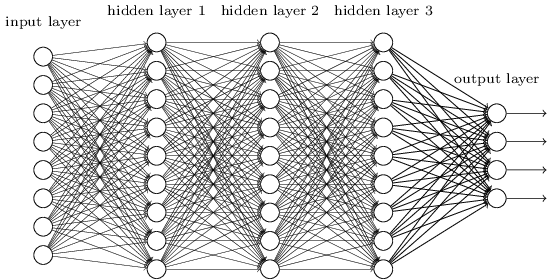
\includegraphics[width=.8\textwidth]{pictures/neural_network}
            \captionof{figure}{Fully-Connected Feed-Forward Network. Image from \cite{nielsenneural}.}
\end{minipage}


Neural network weights are trained with an algorithm called \textbf{Backpropagation}. The backpropagation algorithm is divided into two phases: a forward-pass and a backward-pass.
In the forward pass, the input is propagated throughout every layer and activation until the network's final output is computed. Then the error is calculated, calculating the difference between the network prediction and the training label. In the backward-pass, this error is backpropagated through all the layers to update each neuron's weights.  In the last layer, the update is obtained, calculating the error gradient to understand the change rate of the layer weights. For the hidden layers, instead, the chain rule is applied to propagate the gradient by decomposing the derivative of the produced error recursively with respect to the parameters of the previous layers. 
\\

The standard MLP model has some limitations. After each processed example, the full state of the network is lost. As long as the input data maintains temporal independence between them, there are no problems for learning.
Sometimes instead, the data is correlated, like with video frames or words in a sentence.
In that case, we need a model that can face these correlations even without knowing the input sequence length.
We can extend the "feedforward network," in which the path of the information strictly goes from input to the output by adding a feedback connection in which the information can go back to the model.
This extension allows us to introduce the notion of time to the model.
This new model is called a recurrent neural network (\textbf{RNN}).
In a RNN any state depend from both the current input and the network state in the previous time step.
Lastly, even if the expressive power grows exponentially, both the inference and training grow quadratically, and they are also differentiable end to end, so they are trainable with the backpropagation algorithm.
It is time now to introduce some details of the RNN.
We define a sequence of data as a arrays of data points $x^{(t)}$ extracted from a discrete sequence of \textit{time steps}, each one indexed by t and is expressed with real-valued vectors.
Both the input and the target are represented by a sequence ($x^{(1)},x^{(2)}, ..., x^{(T)}$).

\begin{figure}[h]
\centering
            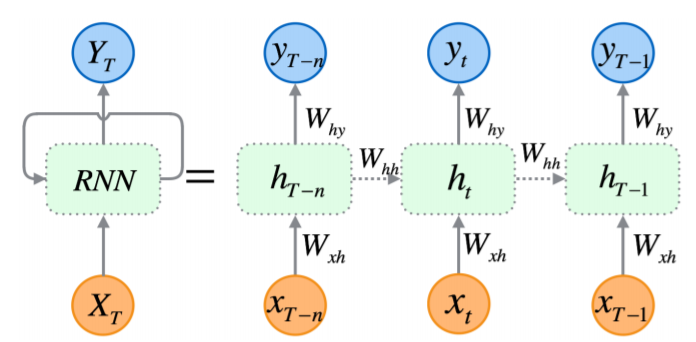
\includegraphics[width=.5\textwidth]{pictures/rnn_schema}
            \captionof{figure}{Standard RNN architecture and an unfolded structure with T time steps. Image from \cite{cui2018deep}.}
            \end{figure}

For each time step $t$ the current node receive information from both the data point $x^{t}$ in input and the previous state $h^{(t-1)}$ from the hidden node.
For each time step $t$, the current node receives information from both the input $x^{t}$ and the previous state $h^{(t-1)}$ and uses this information to update the current state $h^{(t)}$.
$$h^{(t)}=\sigma\left(W^{\mathrm{xh}} {x}^{(t)}+W^{\mathrm{hh}} {h}^{(t-1)}+{b}_{h}\right)$$
This current hidden state $h^{(t)}$ can be used to calculate the current output $y^{(t)}$.
$$\hat{y}^{(t)}=\operatorname{softmax}\left(W^{\mathrm{hy}} h^{(t)}+b_{y}\right)$$
The $W_{hx}$ is the matrix representing the weights from the input and the hidden layer.
The $W_{hh}$ is the matrix representing the recurrent weight between the same hidden layer through different time steps.
During the training, the error signal can be backpropagated through the entire unfolded network across all the time steps.
The backpropagation algorithm, used in a context where time is involved, is called \textit{backpropagation through time} (BPTT).
When we try to backpropagate the error across many time steps we can easily came across a problem of \textit{gradient exploding} or \textit{gradient vanishing}. One possible solution is to limits the maximum number of time steps in which the error can be backpropagated.
This solution is called Truncated backpropagation through time (TBTT).
Another solution is to design a particular architecture to limit the vanishing gradient problem without sacrifice the ability to learn long-range dependencies. 
This second approach led to a new neural network architecture called \textit{Long Short Term Memory} (\textbf{LSTM}) 


        \subsubsection{Long Short Term Memory}

In 1997 Hochreiter and Schmidhuber presented a new RNN architecture called Long Short-Term Memory (LSTM).
In this network, they introduce the memory cell, a new computational unit that replaces the traditional nodes in the network's hidden layers, to handle the vanishing gradient problem of the RNN.
In the traditional RNN, the long memory is maintained through the weights that capture the general knowledge about the data.
The short memory, instead, is represented by the activation function between each successive node.
In the LSTM, the memory cell works like intermediate storage and replaces short and long-term memory.
A memory cell is a composite unit that contains several gates that add or remove information to the cell state.
A gate is a sigmoidal unit that multiplies its output, between 0 and 1, with the value of another node to decide how much information can pass through.
We can describe the works of the LSTM through a sequence of 3 steps: 
\begin{enumerate}
\item \textbf{The Filter}: in the first step, the LSTM decides which information to accept as input and which to forget. To do that it uses the \textit{forget gate} that take in input the current input $x^{(t)}$ and the previous hidden layer $h^{(t-1)}$  and return a vector that will be used later to update the cell state. \\
\begin{minipage}{\linewidth}
            \centering
            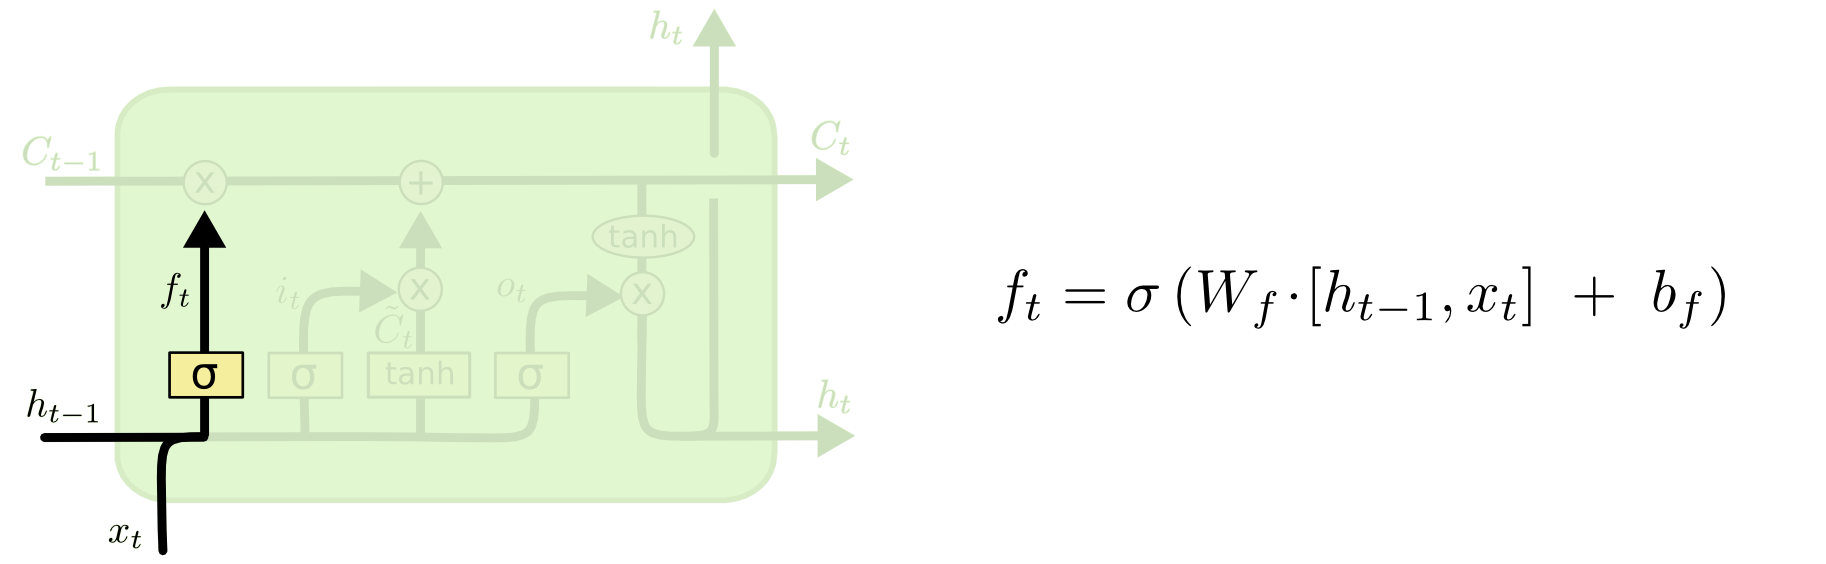
\includegraphics[width=10cm]{pictures/lstm_step1png}
            \captionof{figure}{The output of the sigmoid is a vector of values from zero (completely forget) to one (completely keep). Image from \cite{Colah}.}
        \end{minipage}
		

\item \textbf{The Update}: in the second step, the LSTM decides how much information store in the cell state. This step is divided into two parts: in the first one, it uses the \textit{input gate} to decide what value to update, and a tanh layer is used to create a vector of values called \textit{candidate values} that could be added to the state. In the second one, the LSTM updates its internal state, called \textit{Cell State}. 
			\begin{minipage}{\linewidth}
            \centering
            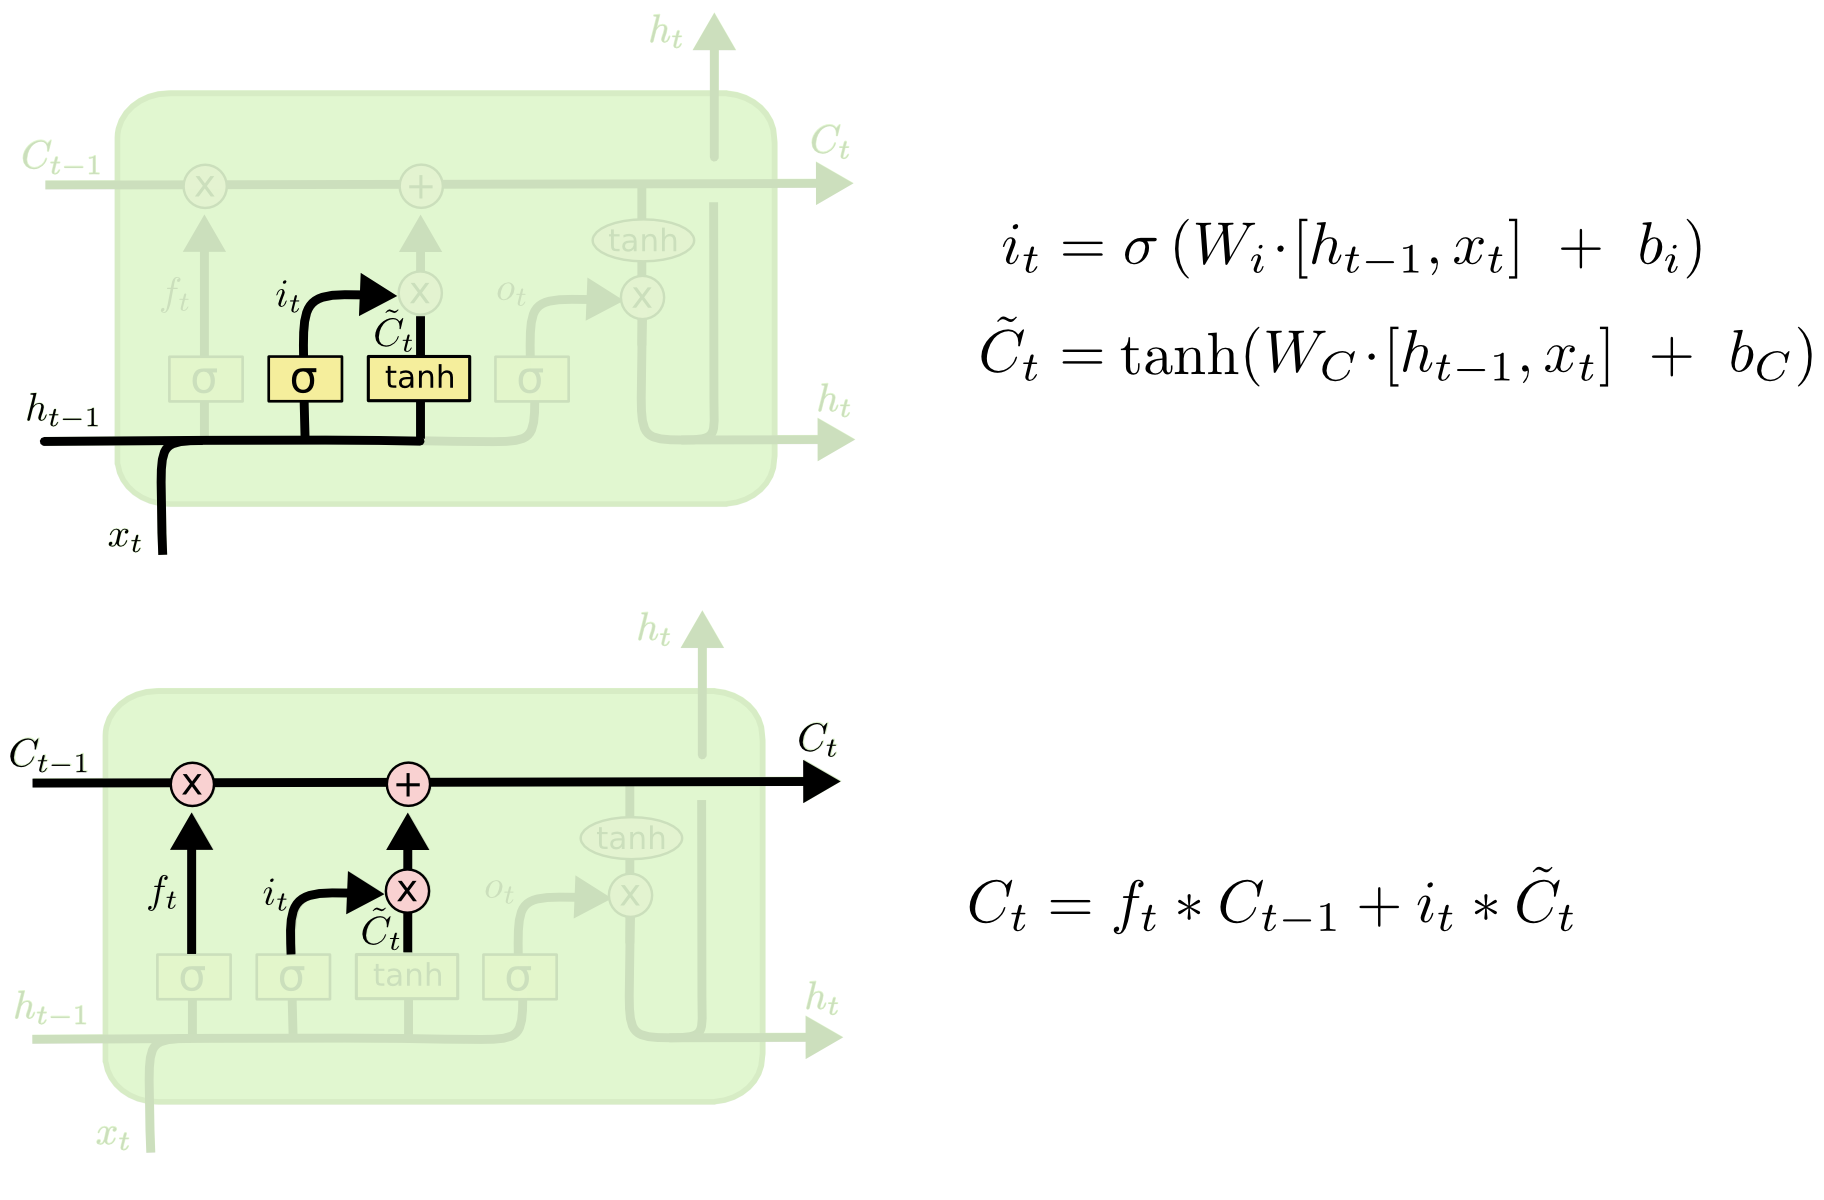
\includegraphics[width=10cm]{pictures/lstm_step2-3}
            \captionof{figure}{The Sigmod layer is used to decide what value to update, the Tanh layer to generate the vector of "candidate values" that could be added to the state. Next decides wich new information ignores, then in the tanh layer, it processes the new information respect the previously hidden layer and with the update gate decides which one to exclude for the update and which ti keep. Now it combines all this information to calculate the new Cell State. Image from \cite{Colah}.}
        \end{minipage}

\item \textbf{Compute Output}: in the final step, the LSTM combine previously hidden value, current input, and current cell state to calculate the new hidden value (that can be viewed as the current network's output). In this step, it is used the \textit{output layer} to decide what part of the state can be outputted.\\
\begin{minipage}{\linewidth}
            \centering
            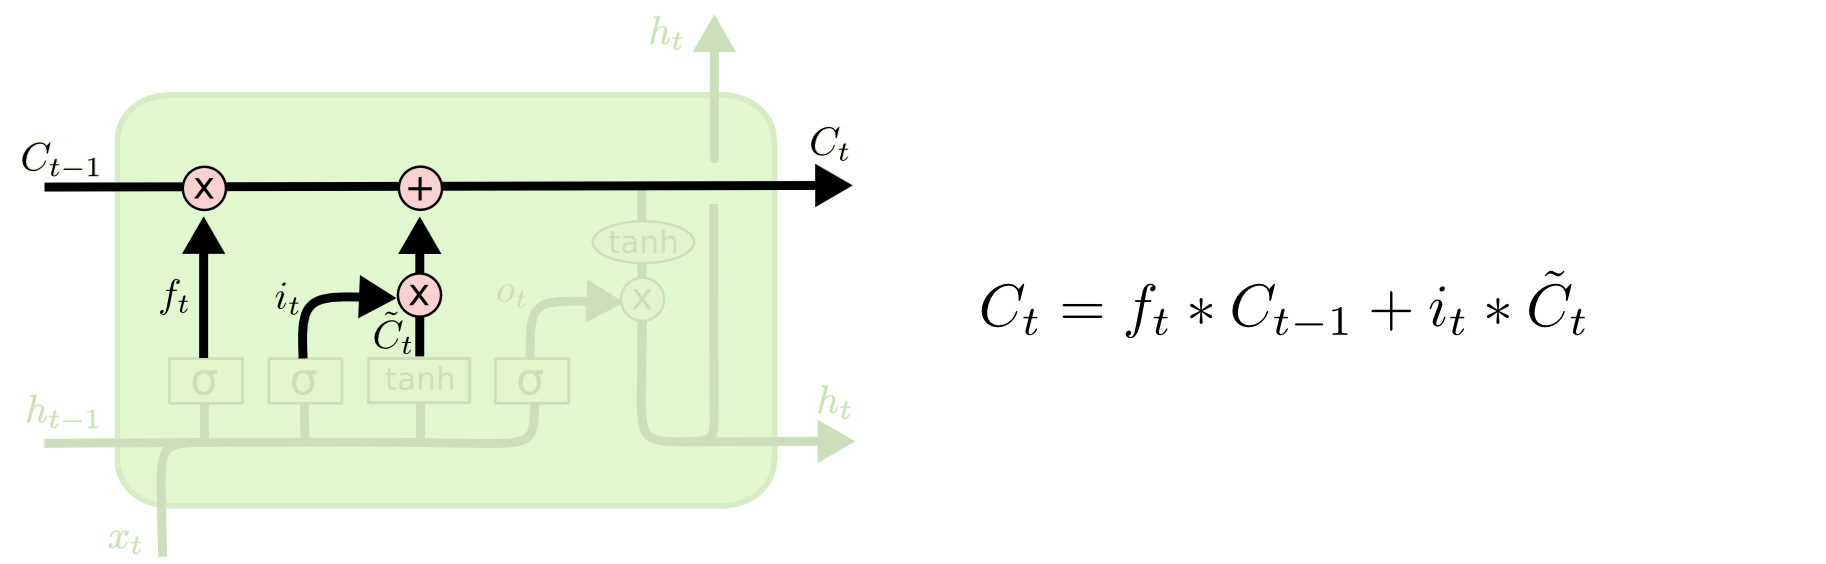
\includegraphics[width=10cm]{pictures/lstm_step3}
            \captionof{figure}{Use the internal state and the output gate to produce the new hidden state. Image from \cite{Colah}.}
\end{minipage}

\end{enumerate}
The LSTM is still used since they have shown a better ability to handle long-range dependencies with respect to the simple RNNs.

\begin{minipage}{\linewidth}
            \centering
            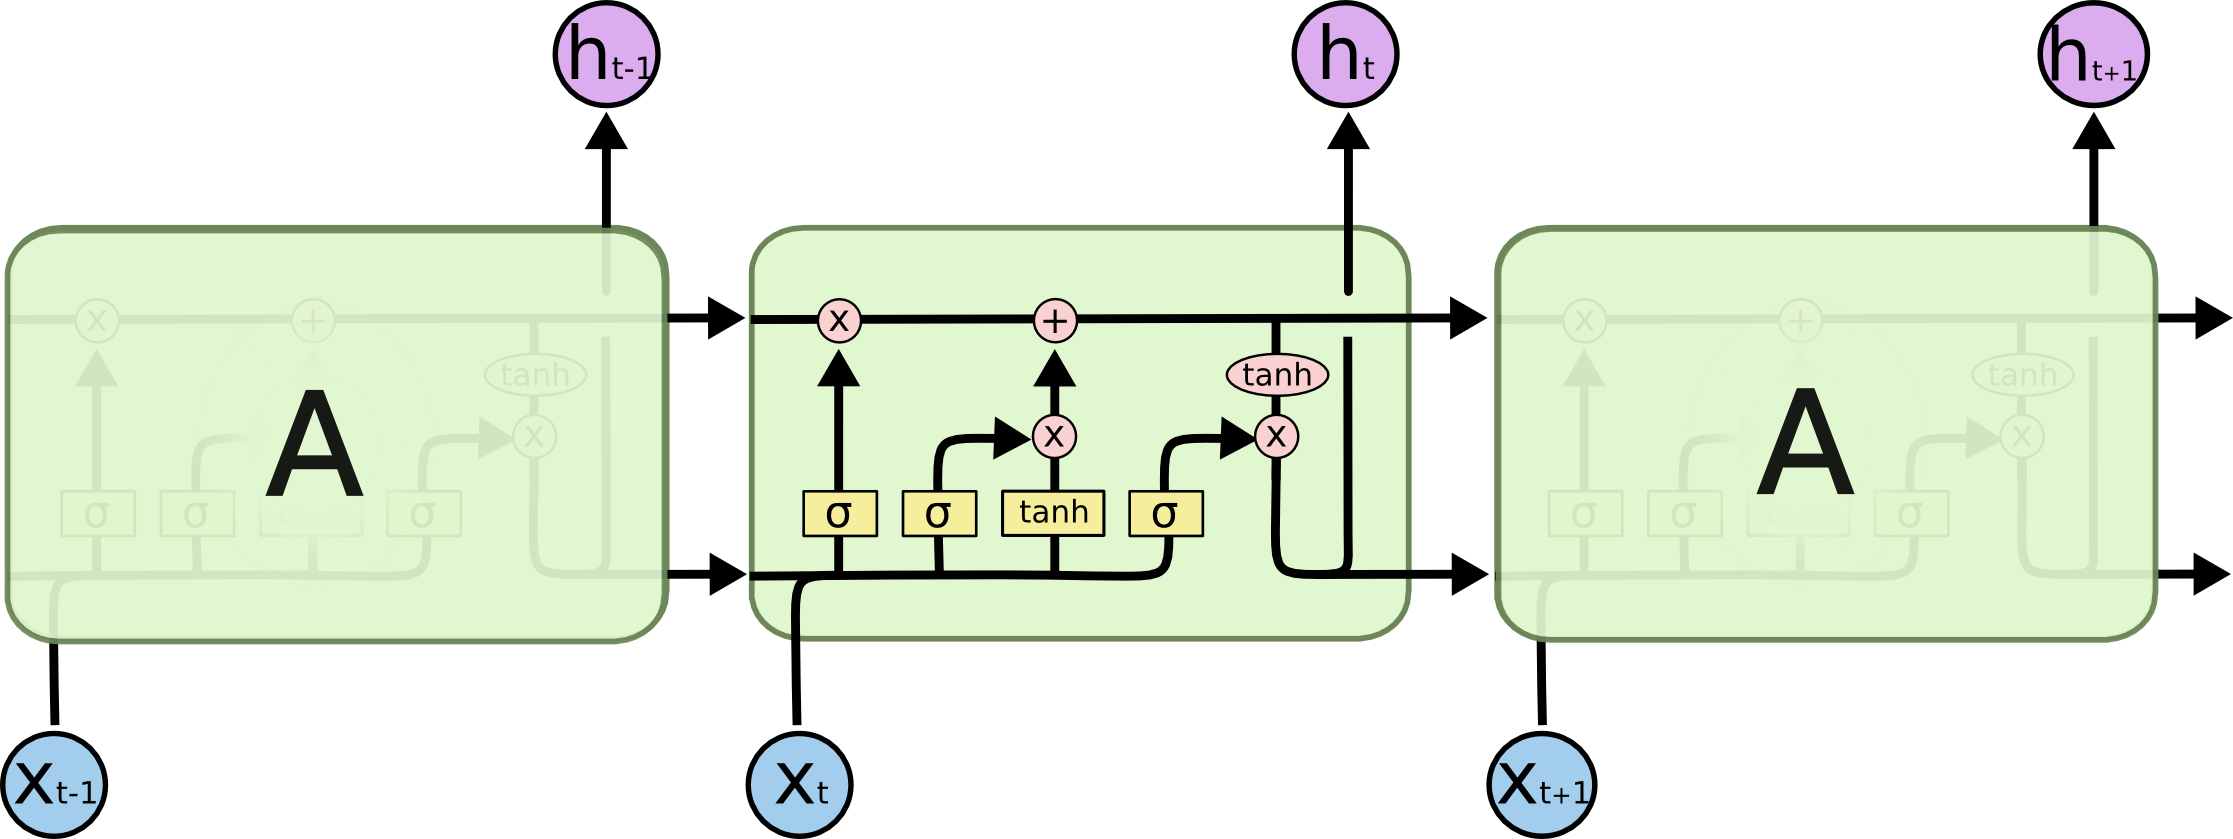
\includegraphics[width=1.0\textwidth]{pictures/lstm_final}
            \captionof{figure}{The LSTM architecture consist on a concatenation of LSTM cell units. Image from \cite{Colah}.}
\end{minipage}


\section{Unsupervised Learning}
The principal tasks of unsupervised learning are:
\begin{itemize}
    \item \textbf{Clustering}: is used to automatically dividing the dataset into clusters of a similar example.
    \item \textbf{Dimensionality Reduction}:  reducing the number of observed random variables in a reduced set of principal variables.
\item \textbf{Generative models}: learning a joint distribution over all the variables. In other words, a generative model simulates how the data is generated in the real world.
\end{itemize}

Recently a new subsets of Unsupervised learning methods has been introduce by Yann LeCun in and it is call \textbf{Self-supervised Learning}. 
According with Longlong Jing and Yingli Tian \cite{jing2020self} 

Self-supervised learning follow the same principle of provide to the learning algorithm a set of pair $X_i$ and $Y_i$ but with the difference that $Y_i$  are automatically generated without involving human annotations. That labels are called psuedo labels.
We introduce one example of this technique: the \textbf{Variational Autoencoder}.

\subsection{Variational  Autoencoder}
Variational  Autoencoder is an example of the class of \textbf{generative model} methods.
Here we provide a general explanation based on the introductory paper \cite{kingma2019introduction}.

In a generative model setting, we try to estimate, explicitly or implicitly, a probability distribution of the data.
Once the generative model has been tuned or trained, we can sample from the estimated distribution and we can generate new input data samples.
The VAE is an implicit generative model, because it produces its own internal representation of the data without producing an explicit formula for the data probability distribution.
For this reason, this model is also used as a method to build a more compact representation of the data, minimizing the information loss.
For the experiments in chapter \ref{Chapter6}, the VAE is used both as a dimensionality reduction algorithm and a generative model.

The VAE represents the marginal distribution over the samples with a function $p_\theta(x|z)$ parameterized with $ \theta $.
This probability is conditionally dependent on the latent variable z.
\begin{equation*}
p_\theta(x) = \int p_\theta(x,z)dz =\int p_\theta(x |z) p(z)dz .
\end{equation*}If we are in a discrete case (so if $z$ is a discrete variable), and $p_\theta(x|z)$ is assumed to be a Gaussian distribution, then $p_\theta(x)$  is a Gaussian mixture distribution.
Instead, if we are working with a continuous variable z, then $p_\theta(x)$ can be seen as an infinite Gaussian mixture distribution.
In this work $z$ is a continuous vector described by a simple Gaussian distribution and $p_\theta(x|z)$ is a conditional Gaussian. 

We need a function that takes all the data in training set as inputs and extract from them the parameters of the latent Gaussian.
Then we can sample the latent vector z from this latent Gaussian.  
We call this function \textbf{encoder} and we formally define it as:
\begin{equation*}
q_\phi(z|x) = \mathcal{N}(\mu_\phi(x),\sigma_\phi(x))
\end{equation*}
Then we need also another function that uses this latent vector z to retrieve x.
We call this function \textbf{decoder} and we formally define it as:
\begin{equation*}
p_\theta(x|z) = \mathcal{N}(\mu_\theta(z),\sigma_\theta(z))
\end{equation*}
In order to find the best parameters $\theta$ we would like to use the Maximum Likelihood principle that is:
\begin{equation}
\label{intractable}
\theta \leftarrow \arg \max_{\theta} \frac{1}{N} \sum_{i} \log \left ( \int p_\theta(x_i|z)p(z)dz \right ).
\end{equation}
Unfortunately, this formula is completely intractable, because of the integral in $ \log\, p(x_i) = \log \int_z p(x_i|z) \, p(x)$, so we need another way.

Before moving on we introduce two concepts that we will use later: entropy and the Kullback-Leibler divergence.

\textbf{Entropy}:  introduced in 1948 by Claude Shannon, the entropy measures the level of uncertainty of a stochastic variable outcome.
For example, an event that has the high probability of occurring, say 90\%, do not give us much information, so it has low entropy.
Instead if we A coin instead, in which all the events have the same probability, will have a high level of entropy.
The formula of the entropy is:
\begin{equation*}
\mathcal{H} = -E_{x\sim p(x)} \left [ \log\, p(x) \right] = - \int_{x} p(x) \log \,p(x) dx
\end{equation*}
\textbf{KL-Divergence}: is a measure of how well a distribution Q approximates another probability P, or in other words, how much information it's lost if the distribution Q is used instead of P.
\begin{equation*}
D_{KL} (P||Q) = E_{x \sim P} \left [ \log \frac{P(x)}{Q(x)} \right] 
\end{equation*}

\begin{itemize}
\item Notice that it is not a distance between two distribution because is not symmetric:\begin{equation*}
 D_{KL}(P || Q) \neq D_{KL}(Q|| P)
 \end{equation*}
\item Where P=Q the KL-divergence is 0:\begin{equation*}
 log  \frac{P}{Q} = log 1 = 0
 \end{equation*}
\item The KL- divergence is always a positive number.
\end{itemize}

Now we can go back to the VAE.
The encoder part is represented by a neural network with parameters $w$, trained to approximate the latent distribution $q_\phi$.
In other words, this neural network will find, from all the training examples x, the respective Gaussian parameters for the latent vector.
So, more formally:
\begin{equation*}
q(z) =  \hat{q}_w(z|x) \approx q_\phi(z|x) 
\end{equation*}
As we have seen before in equation \ref{intractable} it is not possible to use directly that formula.
We need to find another way to define the $\log \, p_\theta(x)$:
\begin{equation*}
    \log\,{p_\theta (x)} = \mathbb{E}_{q_\phi (z|x)} \left[ \log \, p_\theta (x) \right]
\end{equation*}
Now we apply the Bayes's theorem:
\begin{equation*}
p_\theta(x) = \frac{p_\theta(x|z)p_\theta(z)}{p_\theta(z|x)} = \frac{p_\theta(x,z)}{p_\theta(z|x)}
\end{equation*}
and substitute the $p_\theta$(x):


\begin{equation*}
      \log\,{p_\theta (x)} = \mathbb{E}_{q_\phi (z|x)} \left[ \log \left( \frac{p_\theta(x,z)}{p_\theta(z|x)} \right) \right]
\end{equation*}
now we multiply by a constant $q_\phi (z|x)$ (the distribution of the encoder):
\begin{equation*}
      \log\,{p_\theta (x)} = \mathbb{E}_{q_\phi (z|x)} \left[ \log \left( \frac{p_\theta(x,z)}{q_\phi(z|x)} \, \frac{q_\phi(z|x)}{p_\theta(z|x)} \right) \right].
\end{equation*}
next we decompose the expected value:
\begin{equation*}
\log\,{p_\theta (x)} = \mathbb{E}_{q_\phi (z|x)} \left[ \log \left( \frac{p_\theta(x,z)}{q_\phi(z|x)} \right) \right] + \mathbb{E}_{q_\phi (z|x)} \left[ \log \left( \frac{q_\phi(z|x)}{p_\theta(z|x)} \right) \right].
\end{equation*}
We can rewrite the second term as the KL-divergence between $q_\phi$ e $p_\theta$:
\begin{equation*}
\mathbb{E}_{q_\phi (z|x)} \left[ \log \left( \frac{q_\phi(z|x)}{p_\theta(z|x)} \right) \right] = D_{KL} \left ( q_\phi(z|x)||p_\theta(z|x) \right ).
\end{equation*}
Now we focus on the first term:
\begin{align*}
\mathbb{E}_{q_\phi (z|x)} & \left[ \log \left( \frac{p_\theta(x,z)}{q_\phi(z|x)} \right)\right]
\end{align*}
we rewrite the joint probability as a conditional probability:

\begin{align*}
\mathbb{E}_{q_\phi (z|x)} & \left[ \log \left( \frac{p_\theta(x|z)p_\theta(z)}{q_\phi(z|x)} \right)\right]
\end{align*}
we apply the property of logarithms:

\begin{align*}
\mathbb{E}_{q_\phi (z|x)} & \left[ \log\,p_\theta(x|z) \right] -  \mathbb{E}_{q_\phi (z|x)} \log \left ( \frac{q_\phi(z|x)}{p_\theta(z)}   \right)
\end{align*}
we rewrite the second element as a KL-divergence
\begin{align*}
\mathbb{E}_{q_\phi (z|x)} & \left[ log\,p_\theta(x|z) \right] - D_{KL}(q_\phi(z|x)||p_\theta(z))
\end{align*}
Now we can rewrite the entire formula as:
\begin{equation*}
\log_{p_\theta}(x) = \underbrace{\mathbb{E}_{q_\phi(z|x)}[\log \, p_\theta(x|z)]}_{\text=Reconstruction \, error} - \underbrace{D_{KL}(q_\phi(z|x)||p_\theta(z))}_{\text=First \, regularization \, term} + \underbrace{D_{KL}(q_\phi(z|x)||p_\theta(z|x))}_{\text=Second \, regularization \, term}
\end{equation*}
Let us now examine all the components of the formula one by one.

Let's start with the first regularization term. 
It represents the similarity between the encoder and the latent distribution. 
Since both are Gaussians it is possible to calculate the KL in a closed form.

\begin{equation*}
KL(p||q) = \frac{1}{2} \left[ log \frac{\Sigma_2}{\Sigma_1} -d + tr(\Sigma_{2}^{-1}\Sigma_1) + (\mu_2 - \mu_1)^T \Sigma_{2}^{-1} (\mu_2 - \mu_1)\right]
\end{equation*}
The second regularization term instead, represents the similarity between the encoder and the true posterior $p(z|x)$ but it is not possible to calculate it.

We know that the KL divergence is always positive, so we can ignore the second regularization term and obtain a computable lower bound of the $\log\,p_\theta(x)$  that is called Expected Lower BOund (ELBO). 

% RIPARTIRE DA QUI%%
Lastly, we need to find a way to calculate the Reconstruction error term.
This term is the decoder's contribution to the final result: the ability to rebuild x given the latent vector z.
We can approximate it through the sampling and SGD optimization, but we need to introduce a little trick before, called "\textbf{the reparametrization trick}."

We divide the training time into two-phase: forward propagation and backpropagation.

In the forward phase, the encoder produces the parameters for the latent distribution from the given input.
From this distribution, the latent vector is sampled and given to the decoder.
The decoder uses this vector to recreate the original input.
The difference between the decoder's output and the original input is the error of the VAE, and it must be backpropagated for all the computational graph.

In the backpropagation phase, the error passes through the decoder but fails to reach the encoder.
That is because the sampling of z is a non-continuous and a non-differentiable operation; it has no gradient.
So we need to make deterministic the choice of z but to keep stochasticity by applying the reparametrization trick.

\begin{figure}[h]
\centering
\label{reparameterization_trick}
     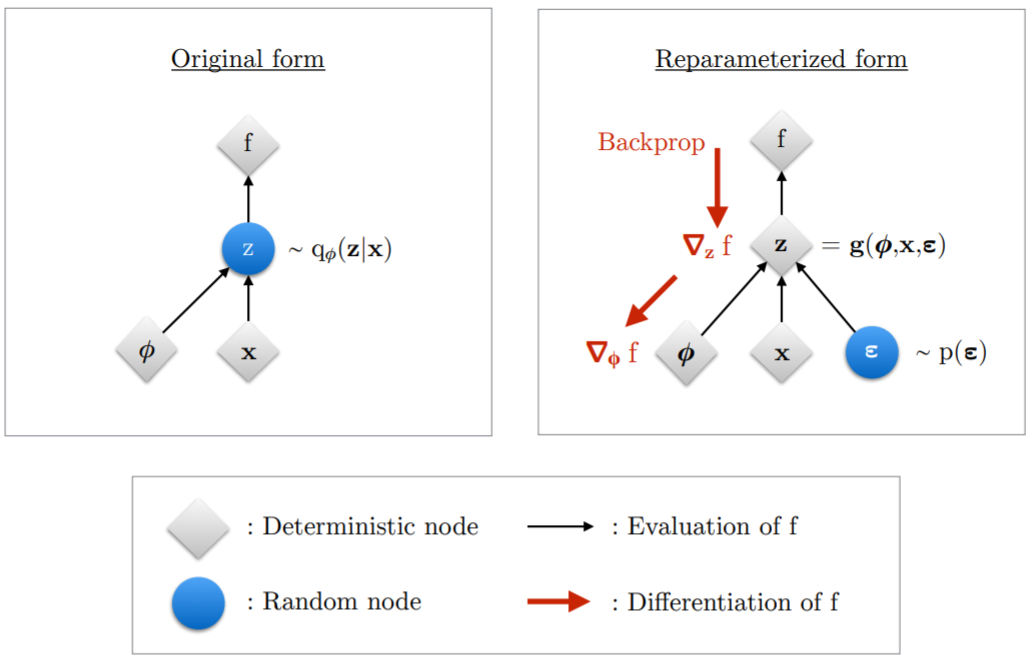
\includegraphics[width=1.0\textwidth]{pictures/reparameterization_trick}
      \caption{Illustration of the reparameterization trick.}
\end{figure}
This method consists of adding a new parameter called $\epsilon$  that is randomly sampled, but that is independent of encoder parameters $\phi$.
\begin{equation*}
\epsilon \sim \mathcal{N}(0,1)
\end{equation*}
Since we cannot directly backpropagate the gradients through the vector z because of its randomness, we re-parameterizing this variable z as deterministic and differentiable.

Now the latent vector is no more sampled but computed:
\begin{equation*}
z = \mu_\phi (x) + \epsilon\sigma_\phi(x)
\end{equation*}
The expectations can be rewritten in terms of $\epsilon$:
\begin{equation*}
\mathrm{E}_{q_\phi(z|x)}[f(z)] = \mathrm{E}_{p(\epsilon)}[f(z)]
\end{equation*}
where $z = g(\epsilon, \phi, x)$.
Finally it is possible to calculate $\nabla_\phi  g(\phi,x,\epsilon)$

\begin{figure}[h]
\centering
     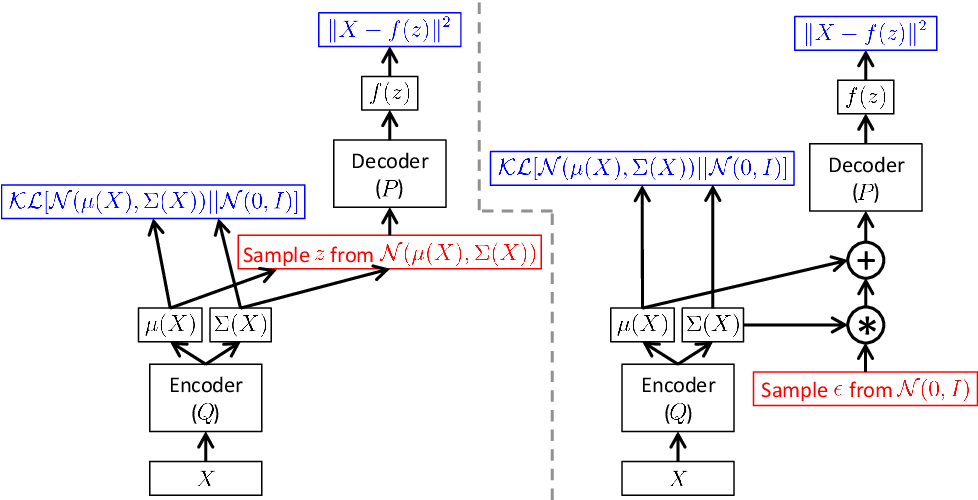
\includegraphics[width=1.0\textwidth]{pictures/vae_struct}
      \caption{A training-time variational autoencoder implemented as a feedforward neural network, where P(X|z) is Gaussian. Left is without the “reparameterization trick”, and right is with it. Image from \cite{doersch2016tutorial}.}
\end{figure}


\section{Reinforcement Learning}
In the reinforcement learning scenario the learner is an agent in an environment. The agent that does not know the environment dynamics, what its purpose is, and obviously how to achieve it.
However, it can choose an action and perform it, and then it will receive a feedback signal that it will use to understand if it was a good or bad action. 

There are infinite possible environments, and for each of them, there are infinite possible objectives. 
Therefore it is necessary to build a method capable of learning in a given environment without any supervision.
The agent's objective function is independent of the environment and it is universal, so it is always the same.
Each agent maximizes the feedback signal and indirectly, in doing so, solves the environment.
The feedback signal is built in such a way that, maximizing it, will lead to resolving the environment. 

Reinforcement learning also differs from unsupervised learning because while the first one is about to maximize a reward signal, the second one is about finding the hidden structure in the collection of unlabeled data.
In the following chapter we explain in more detail the reinforcement learning theory with an explanation of the mathematical preliminaries associated with it.





\clearemptydoublepage
% Chapter 3

\newcommand\tab[1][1cm]{\hspace*{#1}}
\newcommand\Doubletab[1][2cm]{\hspace*{#1}}

\chapter{Elements of Reinforcement Learning} 
\label{Chapter3} % For referencing the chapter elsewhere, use \ref{Chapter3}



In this section, we introduce the basic theoretical concept of reinforcement learning and the mathematical preliminaries associated with it.
In particular, we start from the formalism of MDP and then see as an example one of the first simple approaches to resolution.
For further details, refer to chapter 3,4,5,6 of Reinforcement Learning: An Introduction
\cite{bib:2018Sutton_RLBook}


\section{Markov Decision Process}
In the Reinforcement Learning context, there is an agent that learns how to achieve its goal directly by interaction with the environment. 

\textbf{Markov Decision Processes} formally describe both the environment and the agent. To understand the MDP is necessary to introduce some concepts like \textit{Stochastic Variable}, \textit{Stochastic Process}, \textit{Markov Chain}.

\subsection{Markov Chain}
We start introducing the Stochastic Variable and Stochastic Process.

\textbf{Stochastic Variable}: is a variable, usually expressed with a capital letter, whose possible values depend on a particular outcome of a random phenomenon. 
They are also known as Random Variables and, they can be \textit{Discrete} or\textit{Continuous}.
\\

\textbf{Stochastic Process}: is a collection of discrete stochastic variables each one indexed by a value that represents a step of time in the process.
This index is usually expressed like time step t.
\\

So in a particular time step t, the process is in one of all its possible states mathematically expressed by a stochastic variable.
More formally $s_t \in S$ where $S = \left\{ s_0,s_1, ... , s_m \right\} $.
The set of all possible states is called \textbf{State Space}.

The evolution of the system during the time is represented by a progression of the index from the current variable $s_t$ to the next one $s_{t+1}$.

The rule by which the index progress is called  \textbf{Transition Function}, and it is not deterministic, so the process produces different sequences of states each time it is run, even if it always starts from the same initial state.
The value of a variable can influence that of the variables that follow it. 
Therefore the progression of the states depends on the whole sequence starting from the initial state.
More formally this rule is expressed with a probability distribution: $$ P[S_{t+1} | S_1, ..., S_t] $$



A \textbf{Markov Chain} is a particular case of stochastic process that respects the Markov Property: "The future is independent of the past given the present".

This means that each state must capture all the relevant information from the environment at that moment, so when you have the state, you could throw away all the history.
In other words, thanks to the Markov Assumption the transition function is conditionally independent from the past state if the current state are given.

More formally we say:
\begin{equation*}
    P[S_{t+1} | S_t] = P[S_{t+1} | S_1, ..., S_t] 
\end{equation*}    


\subsection{Markov Decision Process}
A Markov Decision Process (MDP) is an extension of the \textit{Markov Chain} that includes an agent that performs actions in the process, that in this context is called \textbf{Environment}.


The agent influences the evolution of the environment with its actions.
So the state transition probability change including also the actions: $P(s, a, s^{'}) = [S_{t+1} = s' | S_t = s, A_t = a] $.
The purpose of the agent is to led the evolution of the environment to a particular set of states, called \textbf{Goal States}.
At every time step, the agent makes a decision on which is the best action to take.
The process by which the agent chooses an action from the given state is represented by with a function, called \textbf{Policy Function}.
It is represented by a probability distribution associated with every state in input. 
More formally we say: an agent follows the policy $\pi$ for every time step $t$ and for each $s_t \in \mathcal{S}$ it executes the action $a_t \in \mathcal{A}$ according to the probability $\pi(a|s)$.
To guide the agent's decision process we assign a reward signal (a real number $r_t\in 	\mathbb{R}$) to every action that it executes. 
Having this reward signal we can say if a state is more desirable then one other.



\begin{figure}[h]
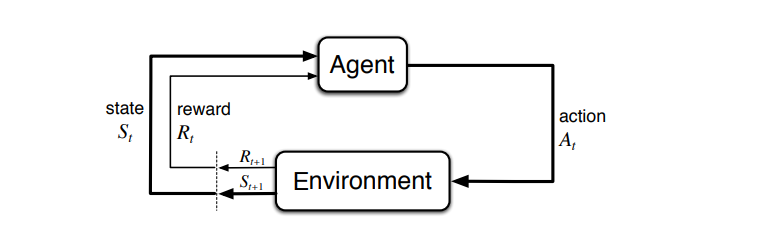
\includegraphics[width=\textwidth]{pictures/mdp_schema}
\caption{The agent-environment interaction in a Markov decision process. (Image source: Sec. 3.1 Sutton and Barto (2017) \cite{bib:2018Sutton_RLBook}}
\centering
\end{figure}


The agent receives the initial state of the environment and uses it to choose an action. 
Then, the environment evolves its state into a new one depending on both the current state and the agent's action. 
At this point, the agent receives two inputs: the new state and the reward signal.
It uses the reward signal to improve its own decision method and the new state to choose the next action.

This process is repeated iteratively until a final state is reached.

Every step of this process is called \textbf{Transition}: ${s_t,a_t,r_t,s_{t+1}}$.
The list of all transition from initial state to the final one is called \textbf{Episode}.

There are some particular classes of MDP that are called \textbf{Infinite MDP} in which do not exist a final state, but the construction of the reward function is still possible.

The agent can use the reward signal to know what is a good move and what it isn't.
With this knowledge, it can learn the best strategies to achieve its goal.
Assuming to be in a particular time step t of a finite MDP the definition of cumulative reward, from step t to the final step T, is:

\begin{equation*}
G_t = R_{t} + R_{t+1} + R_{t+2} + ... + R_{t+T}  
\end{equation*}
So the objective of the reinforcement learning is to find the parameters $\theta^*$  to the policy function $\pi^*$ that maximizes the expected cumulative reward of all the episodes.
\begin{equation*}
\label{policy_function}
    \pi^* = argmax_\theta E_{\tau \sim \pi_\theta} \left [\sum_{t}^{T}    r(s_t, a_t)  \right ]
\end{equation*}

The reward value is often presented with the \textbf{Discount Factor}, generally expressed with the symbol $\gamma \in [0,1]$. 
The purpose of the discount factor is to define the priority that the agent assigns to the future expected reward with respect to the immediate ones.
So the formula of the discounted expected cumulative reward becomes:

\begin{equation*}
G_t = R_{t} + \gamma R_{t+1} + \gamma^2 R_{t+2} + ... = \sum_{k=0}^\infty \gamma^k R_{t+k} 
\end{equation*}


Notice that the lower the gamma factor is and the more the agent will prefer the immediate reward than the long term values. 

This value not only helps to represent the uncertainty about the future but it is also mathematically convenient because it can be used to end up with a finite number also in case of infinite sequence of states (using the sum of infinite series) if $\gamma < 1$. 
So it can be very useful for Infinite MDP. 





To conclude a MDP is a tuple defined by $<\mathcal{S},\mathcal{A},\mathcal{P},\mathcal{R}, \mathcal{Z}, \gamma>$:
\begin{itemize}
  \item a finite set of states $\mathcal{S}$ 
  \item an initial state $s_0$
  \item a finite set of actions $\mathcal{A}$
  \item a state transition probability $P(s, a, s^{'}) = [S_{t+1} = s' | S_t = s, A_t = a] $
  \item $\mathcal{R}$ is a reward function, $\mathcal{R}(s,a)$ 
  \item $\gamma$ is a discount factor $ \gamma \in [0,1].$
\end{itemize}



\subsection{Partially Observable Markov Decision Process}
A Partially Observable Markov Decision Process, also called POMDP, is a particular case of MDP in which the agent hasn't direct access to the full states but for each time step,it makes an observation that depends on it. 

A POMDP in defined by a tuple $<\mathcal{S},\mathcal{A},\mathcal{P},\mathcal{R},\mathcal{Z},\gamma>$, so respect to the classic MDP it required also:
% \mathbb{R} set of real numbers
\begin{itemize}
  \item a finite set of observations O
  \item an observation function, $\mathcal{Z}(o,a,s^{'}) = P\left [O_{t+1} = o | S_{t+1} = s^{'}, A_t = a \right]$
  
\end{itemize}

In POMDP the transition is composed by the action, the reward and the observation of the environment. 
We define the entire sequence, from initial state to some time step t, as history $H_t$:

\begin{equation*}
    H_t = O_0, A_0, R_0, O_1, \dots, O_{t-1}, A_{t-1}, R_{t-1}, O_{t}
\end{equation*}

During the history, the agent formulates hypothesis on what is the effective state behind each observation. To build this hypothesis, that is called \textit{belief state}, it uses the history.

So, more formally, a belief state b(h) is a probability distribution over states, conditioned on the history h:

\begin{equation*}
b(h) = \left (P\left[ S_t = s^{1} | H_t = h \right] , ... , P\left[ S_t = s^{n} | H_t = h \right]\right) 
\end{equation*}
With the belief state the Markovian Assumption is no more valid.

\section{Solving Markov Decision Process}
In this section we introduce the two principal approach to solve an MDP, that are called \emph{prediction problem}, used when a fixed policy is given and \emph{control problem} used when there are no policy available. 

\subsection{Prediction Problem}
The prediction problem consist of evaluating a given policy function in an unknown MDP.
The metric used to evaluate a policy is the \textbf{value function}.

For every state the value function estimates how good it is for the agent that follows its given policy in the environment.
This value is a scalar number and it is expressed in terms of the expected cumulative discounted reward from the given state to the end.  
So, more formally:
\begin{equation*}
v_\pi(s) = E_\pi \left[ G_t | S_t = s \right]. 
\end{equation*}

To explain how it works we first need to define a partial ordering over policies. 
One policy is better than another when it produces a greater value for each state. 
More formally: 
\begin{equation*}
\pi \geqslant \pi^{'} \forall s \in \mathcal{S} \iff v_\pi(s)  \geqslant  v_\pi'(s) \, \forall s \in \mathcal{S}
\end{equation*}
So also the definition of the best policy is related to the value function:
\begin{equation*}
\pi_* \geqslant \pi \, \forall \pi \, (\forall s \in S) \iff v_*(s)  \geqslant  v_\pi(s)\, \forall s \in \mathcal{S}
\end{equation*}

From Sutton's book \cite{bib:2018Sutton_RLBook}, in chapter 3.6, we can read: "there is always at least one policy that is better than or equal to all the other policies. This is an \textbf{optimal policy}." 
Starting from the definition of the value function, it is possible to derive the iterative formulation for any arbitrary state.

\begin{align}
    v_\pi(s) &= E_\pi \left [ G_t | S_t = s \right ] \\
    v_\pi(s) &= E_\pi \left [ R_{t} + \gamma G_{t+1} | S_t = s \right ] \\
    v_\pi(s) &= \sum_{a}\pi(a|s)\sum_{s^{'}}\sum_{r}p(s^{'},r|s,a)\left [ r + \gamma E_\pi \left [ G_{t+1} | S_{t+1} = s^{'} \right ] \right ] \\
    \label{bellman-equation}
    v_\pi(s) &= \sum_{a}\pi(a|s)\sum_{s^{'},r}p(s^{'},r|s,a) \left [ r + \gamma v_\pi(s^{'})  \right ]
\end{align}
The equation \ref{bellman-equation} is the \textbf{Bellman equation} for $V_{\pi}(s)$ and it shows the relation between the value of one state and the value of its successor. 
"It states that the value of the start state must equal the (discounted) value of the expected next state, plus the reward expected along the way" \cite{bib:2018Sutton_RLBook}.
From there, it is possible to derive the \textbf{Bellman Optimality Equation} used to calculate the optimal value function $v_*$. 
Note that this equation can be written independently to any particular policy.
Intuitively, the best policy must suggest the action with the highest expected return from the given state.
Therefore the optimal policy evaluation consist of finding the action that maximizes the value function of the successor state plus the expected reward obtained from the actual states to the next one s'.
\begin{equation*}
v_*(s) = \underset{a}{\max} \sum_{s^{'},r}p(s^{'},r|s,a) \left [ r + \gamma v_*(s^{'})  \right ]
\end{equation*}


\subsection{Control Problem}
The \emph{control problem} consist of solving an MDP without a given policy.
The metric used to build an effective policy is the \textbf{Q-Value function}.

The q-value, defined $q_\pi(s,a)$ is the expected discounted return after executing the action $a$ from $\pi(s|a)$ and then keeping to follow the actions from the policy $\pi$. 
It is also called \textit{action-value function}. 
More formally, we define the \textit{action value function for the policy $\pi$}, $q_\pi$, as follows:
\begin{align}
\label{q-value}
q_\pi(s,a) &\doteq  E_\pi \left[ G_t | S_t=s, A_t = a \right] \\
q_\pi(s,a) &\doteq E_\pi \left[ \sum_{k=0}^{\infty}\gamma^k R_{t+k} | S_t = s, A_t = a \right] 
\end{align}
The optimal Q-Value can be defined as:
\begin{equation*}
q^*(s,a) =  \underset{a\in A(s)}{max} q_{\pi^{*}}(s,a),	\quad\forall  s \in S, a \in A
\end{equation*}
It is also possible to write the $q_*$ in terms of $v_*$ as follows:

\begin{equation}
\label{bellman-equation-for-q}
q_*(s,a) = E \left [  R_{t+1} + \gamma v_*(S_{t+1}) | S_t = s, A_t = a \right]
\end{equation}
From the last equation is possible to derive the \textbf{Bellman optimality equation} for $q_*$.
Starting from $v*$:

\begin{align*}
v_*(s) =&  \underset{a\in \mathcal{A}(s)}{\max}q_\pi*(s,a)\\
v_*(s) =& \underset{a}{\max} E_{\pi_*} \left[  G_t | S_t = s, A_t = a \right]\\
v_*(s) =& \underset{a}{\max} E_{\pi_*} \left[ R_{t} + \gamma G_{t+1} | S_t = s, A_t = a \right]\\
v_*(s) =& \underset{a}{\max} E_{\pi_*} \left[ R_{t} + \gamma v
(S_{t+1}) | S_t = s, A_t = a \right]\\
\end{align*}
Now we can apply the previous formula:
\begin{align} \label{q_star}
q_*(s,a) =& E \left[ R_{t+1} + \gamma \, \underset{a^{'}}{\max} \, q_* (S_{t+1}, a^{'}) | S_t = s, A_t = a   \right] \\
q_*(s,a) =& \sum_{s^{'},r}p(s^{'},r|s,a)\left[ r + \gamma \, \underset{a^{'}}{\max} q_*(s^{'},a^{'})\right]
\end{align}
Starting from a given state, the agent must find the action that maximizes $ q _ * (s, a) $ without the knowledge of the possible successor states or the dynamics of the environment.

It's time to use all the information introduced in this chapter to show how to build the policy function.
This method is called \textbf{Generalized Policy Iteration} (GPI) and it is the combination of two interacting processes called \textbf{Policy Evaluation} and \textbf{Policy Improvement}.

\begin{figure}[h]
\centering
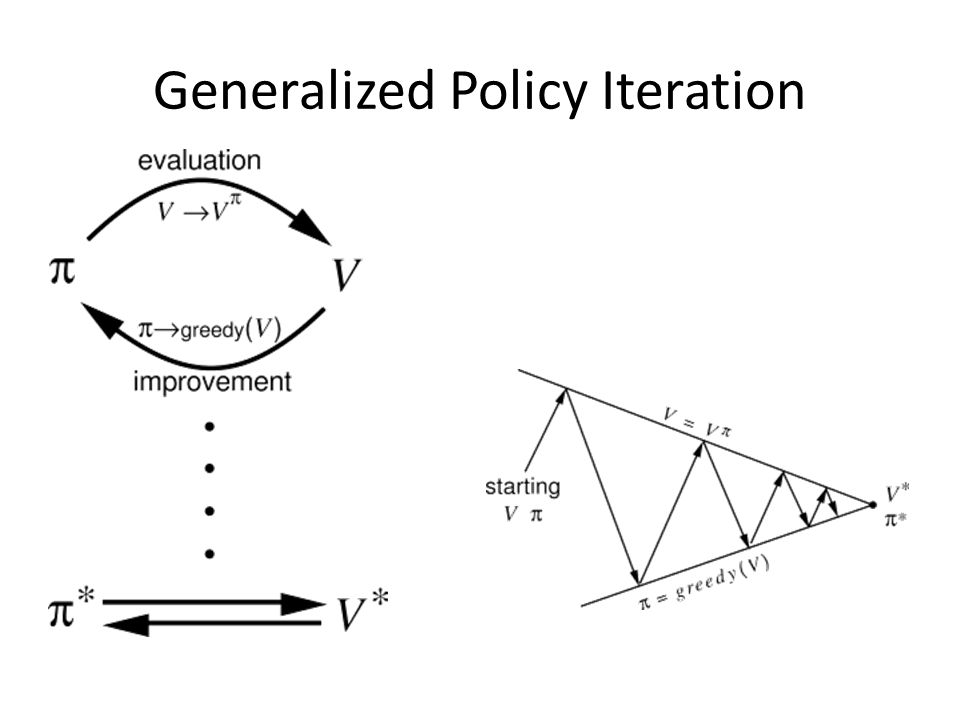
\includegraphics[width=.75\textwidth, height=.4 \textheight]{pictures/gpi_schema}
\caption{The GPI schema. (Image source: Sec. 4.6 Sutton and Barto (2017) \cite{bib:2018Sutton_RLBook}}
\end{figure}

The first process makes the value function consistent with the current policy computing the $V_\pi$.
\begin{align*}
V_{\pi}(s) =& E_\pi \left[  r + \gamma V_\pi(s^{'}) | S_t = s \right]
\end{align*}
The second process use the current value function to greedily  improve the policy:
\begin{align*}
Q_\pi(s,a) =& E\left[ R_{t+1} + \gamma V_\pi(S_{t+1}) | S_t = s, A_t = a \right]
\end{align*}
As said before, the GPI algorithm iterate over these two processes until it reaches convergence.
\begin{equation*}
\pi_0 \xrightarrow[]{\text{evaluation}} V_{\pi_0} \xrightarrow[]{\text{improve}}
\pi_1 \xrightarrow[]{\text{evaluation}} V_{\pi_1} \xrightarrow[]{\text{improve}}
\pi_2 \xrightarrow[]{\text{evaluation}} \dots \xrightarrow[]{\text{improve}}
\pi_* \xrightarrow[]{\text{evaluation}} V_*
\end{equation*}
\section{Taxonomy of Reinforcement Learning Algorithms}
\label{taxonomy}
Since the dynamics of the environment is not know, it is impossible to calculate directly the value or q-value function. 
For this reason there are two methods to approximate them, that are called \textbf{Monte Carlo Methods} (MC) and \textbf{Temporal Difference Methods} (TD).

Monte Carlo methods are based on the idea of repeated random sampling to estimate a distribution function. 
In this context, the function to approximate is the value functions need to the GPI schema explained in previous section.
In order to compute the policy evaluation step, the agent performs several rollouts of the current policy accumulating the reward and the visited states of the entire episodes. 

To accomplish the policy evaluation phase, the agent interacts with the environment accumulating experience.
Every time it visits a state, it takes note of the number of times it encounters that state ($N_ {(n)}$) and the cumulative reward obtained in that episode from that state to the end ($C_ {(n)}$).
\begin{align*}
N_{(s)} &\leftarrow N_{(s)}+1 \\
C_{(s)} &\leftarrow C_{(s)} + G_t
\end{align*}
Now having the number of times the agent has visited a state and the cumulative total reward, it is possible to approximate the value function for each state by calculating the mean return.
\begin{equation*}
V_{(s)} \leftarrow C_{(s)}/N_{(s)}
\end{equation*}
In the policy improvement step the agent chooses the action greedily with respect to the value function.
\begin{equation*}
\pi^{'}(s) = \underset{a\in A} 	\max Q(s,a)
\end{equation*}
These two steps are iteratively repeated, and it can be shown that using the law of large numbers, it is possible to prove that the algorithm converges to the optimal policy and the optimal value function.
\begin{equation*}
V_{(s)} \rightarrow v_\pi(s) \, as \, N(s) \rightarrow \infty
\end{equation*}
The problem with the Monte Carlo method is that it requires to finish the entire episode before to update the value function.

\textbf{Temporal Difference (TD)} methods are also based on the idea of GPI but differ from MC methods in the Policy Evaluation phase.
Instead of getting to the end of the episode, these methods update the value function step by step.
These methods use the current temporal estimates of the state value function, rather than relying on the complete return as the MC methods. 
This approach is called \textbf{bootstrapping}.
To obtain a better approximation the algorithm recalculate the value of every state it visits and it adds to it the reward occured in that transiction, forming the so called \textbf{TD target}.
The TD target is a slightly better approximation of the state value for that state, so the approximation must move in that direction.
To move the approximation it's necessary to calculate di difference between the old estimation and the new one, producing the \textbf{TD error}.
The entity of the update is controlled by a hyperparameter called learning rate $\alpha.$
So, this processes is repeated at each time step, and the value function is continually update.
This is called \textbf{online update}.
The formula for the value function is:
\begin{equation*}
V(S_t) \leftarrow V(S_t) + \alpha(R_{t+1} + \gamma V(S_{t+1}) - V(S_t))
\end{equation*}
The formula for the q-value function is:
\begin{equation}
\label{q-update}
Q(S_t,A_t) \leftarrow Q(S_t,A_t) + \alpha(R_{t+1} + \gamma Q(S_{t+1},A_{t+1}) - Q(S_t,A_t))
\end{equation}
These methods are referred to as \textbf{Tabular Methods} because the temporal results are cached in a table. 

The most famous algorithm in this category is \textbf{Q-learning}.  \cite{watkins1992q}.
The formula used in this algorithm to update the Q-value estimate is the equation  \ref{q_star}  that we already presented before:
\begin{align*}
q_*(s,a) =&  E\left[ R_{t+1} + \gamma  \underset{a^{'}}{\max} \, q_*\left (S_{t+1}, a^{'} \right) | S_t = s, A_t = a   \right] \\
\end{align*}
For the online update version of this formula the expectation is removed, so the formula became:
\begin{align*}
Q(s,a) =& R(s,a) + \gamma  \left(  \underset{a'}{\max}Q (s',a') \right) 
\end{align*}
Applying this TD target to the generic version of the TD formula:
\begin{align*}
Q(S_t, A_t) &\leftarrow Q(S_t, A_t) + \alpha (R_{t+1} + \gamma \max_{a \in \mathcal{A}} Q(S_{t+1}, a) - Q(S_t, A_t)) \\
\end{align*}



The formula \ref{q-update} the Q-learning formula add a $max$ operation, this simplifies the algorithm approximating the optimal action-value function, $q_*$, directly.


    \begin{algorithm}[H]
        \begin{algorithmic}
          \State Initialize $Q(s, a),$ $ \forall s \in \mathcal{S}, a \in \mathcal{A}(s),$ arbitrarily, and $Q($terminal-state$, \cdot)=0$
          \State Repeat (for each episode):
          \\\tab{Initialize $\mathcal{S}$}
          \\\tab{Repeat (for each step of episode):}
		  \\\Doubletab{ Choose $\mathcal{A}$ from $\mathcal{S}$ using policy derived from $\mathbf{Q}$ (e.g., $\epsilon-greedy$)}
          \\\Doubletab{Take Action $\mathcal{A}$, observe $\mathcal{R}$, $\mathcal{S'}$}
          \\\Doubletab{ $Q(S, A) \leftarrow Q(S, A)+\alpha\left[R+\gamma \max _{a} Q\left(S^{\prime}, a\right)-Q(S, A)\right]$}
          \\\Doubletab{ $\mathcal{S} \leftarrow \mathcal{S'}$}
          \\\tab{until $\mathcal{S}$ is terminal}
        \end{algorithmic}
    \caption{Q-learning (off-policy TD control) for estimating $\pi \approx \pi_{*}$}
    \label{alg:q-learning}
    \end{algorithm}


Both the MC and TD methods are also \textbf{Model-Free algorithms} because they solve the MDP, calculating the value or q-value function, without knowing the environment dynamics. 

However, an agent could also learn the transition probability function and the reward function and use them to accelerate the learning process or build a long term plan before acting. 
In that case, we talk about the \textbf{Model-Based algorithms} in which the model is learned, not given.

Another classification is based on how the methods find the best action to take.
The option are \textbf{Value function based} or \textbf{Policy function based}.
All the methods presented so far are value based: these methods learn the value function and then use it to choose the action with the best result.
The policy function based, instead, search directly in the policy parameters space and ends up with the best policy.

Finally there is the \textbf{Actor-Critic} method that build both the value and the policy functions.

This method is composed by two element: the actor and the critic.
The Actor is the Policy function and decides which action to take and the Critic is the Value function approximation and tells the actor how good its choice was and how to adjust it.



The critic updates value function parameters and the Actor update policy parameter using the value function suggested by the critic. 

\begin{figure}[h]
\centering
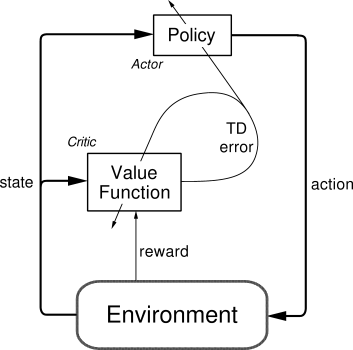
\includegraphics[width=.9 \textwidth, height=.6\textheight]{pictures/ac_schema}
\caption{ The actor-critic architecture. [Image source: Sec. 6.6 Sutton and Barto (2017)  \cite{bib:2018Sutton_RLBook}]}
\end{figure}
In the next chapter, we will introduce an actor-critic method called DDPG that will be use it to do the experiments. In chapter \ref{Chapter6}, we compare the results obtained with DDPG and the results obtained with a model-based algorithm called PlaNet.  

\clearemptydoublepage
% Chapter 4

\chapter{Model Free Reinforcement Learning} % Main chapter title

\label{Chapter4} % For referencing the chapter elsewhere, use \ref{Chapter1} 

\section{Deep Reinforcement Learning}
\subsection{Deep Q Network}

As we so in chapter \ref{Chapter3}, to solve an unknown MDP, we use the Bellman equation \ref{bellman-equation-for-q}.
We want to approximate the function of the optimal value iteratively until the algorithms converge, but to do this, we need to maintain the experience gained in the previous iterations.
Originally, all the temporary q-value estimates were stored in a tabular, but this kind of solution worked well only with toy problems.
The solution was the use of a function approximator instead of tabular methods.
Initially, they tried whit a linear function approximation, but also that solution is not able to scale.
The first, scalable and successfully, use of neural networks as a function approximator of Q-value was introduced in 2015 by Deepmind \cite{mnih2015human}.
The solution proposed in this work is to build a Q-network and train it by adjusting the parameters $ \theta $ to reduce the mean-squared error in the Bellman equation.

This network, called \textbf{Q-Network}, takes an observation as input and then give in output, with a single forward pass, the predicted Q-values for all possible actions.

Before this solution, the use of neural networks in the framework of reinforcement learning was known to be an unstable method.
This instability has several causes: the correlation between transactions, the change in the distribution of data caused by the change in policy.
To address these problems, they introduce two variants of the q-learning algorithm. 

An \textbf{Experience Buffer Replay} was introduced to remove correlations in the observation sequence and smooth over changes in the data distribution.

So, at each time step $t$, the agent store its experience $e_t=(s_t,a_t,r_t,s_{t+1})$ in a dataset $D_t={e_1, ... ,e_t}$.
At the learning time it the agent draw a random batch of experiences from the dataset and apply a Q-learning update.  

The second variant is the use a second neural network called \textbf{Target Network} to perform a target estimate in the Q-update.
So the Q-network is trained to reach the target network predictions that use an old set of weight.
So, every C updates the Q-networks weights are cloned to generate a better set of weights for the Target-networks.
This solution makes divergence or oscillations much more unlikely.

This algorithm was tested on a set of environments that replicated the games from an old console called atari Atari 2600.
Reinforcement learning was usually applied to domains in which useful features were being crafted in low-dimensional state space.
The DQN instead, was trained directly from high-dimensional inputs that were the raw frames of the games. 

This choice led to a problem, one single frame does not contain enough information to be an effective state of an MDP since it violates the Markov property.
In fact, having one single frame is not enough to
predict the next one (for example, you cannot guess the position of an object in the next frame if you do not know its speed and direction).
So, in that case, the environment is not an MDP but is a POMDP.
To give to the network enough information they stacked more frames into one single input.

Using the frames as input allow the algorithm to be more general.
In fact, DQN was able to achieve human-level performance over 49 different games using the same network architecture and hyperparameters.

\begin{algorithm}
	\caption{Deep Q-learning with Experience Replay}
	\label{algo:DQN}
	\begin{algorithmic}[]
		\State initialize replay memory \textit{D} to capacity {N}
		\State initialize action-value function \textit{Q} with random weights {$\theta$}
        \State initialize target action-value function ${\hat{Q}}$ with weights ${\theta^-}={\theta}$
		 \For{episode=1,M}
			\State Inizialize sequence $s_1$=$x_1$ and preprocessed sequence $\phi_1= \phi(s_1)$
            \For{$t = 1,T$}
            		\State With probability $\epsilon$ select a random action $a_t$ 
                   \State otherwise select $a_t = argmax_aQ(\phi(s_t),a;\theta)$
                   \State Execute action $a_t$ in emulator and observe reward $r_t$ and image $x_{t+1}$
                   \State Set $s_{t+1} = s_t,a_t,x_{t+1}$ and preprocess $	\phi_{t+1} = \phi(s_{t+1})$
                   \State Store transition $(\phi_t,a_t,r_t,\phi_{t+1})$ in D
                   \State Sample random minibatch of transitions $(\phi_j,a_j,r_j,\phi_{t+1})$ from D
                   \If{episode terminates at step j + 1}
                   \State set $y_j = r_j$
                   \Else
                   \State set $y_j = r_j+\gamma\,max_a'\hat{Q}\left (\phi_{j+1},a';\theta^- \right)$
                   \EndIf
                   \State Perform a gradient descent step on $\left ( y_j - Q \left( \phi_j,a_j,\theta \right) \right)^2$ 
                   \State with respect to the network parameters $\theta$
                   \State Every C steps reset $\hat{Q}=Q$
               
                   
                    
        	\EndFor    
        \EndFor
	\end{algorithmic}
\end{algorithm}

\section{Policy Gradient}
In chapter \ref{taxonomy} we have introduced the difference between \textbf{Value function} based methods and \textbf{Policy function}. 
DQN is the most famous example of an algorithm based on Value function.
The Policy function methods instead, do no approximate a value function but learn directly the policy as $\pi(a|s;\theta)$. 
The objective is to maximize the expected reward cumulated during the episode.
We now introduce \textbf{REINFORCE}, one of the algorithms based on this method, also called Monte-Carlo policy gradient.


\subsection{REINFORCE algorithm}
As we said we want to maximize the expected cumulative reward 
\begin{equation*}
\theta^* = \underset{\theta}{argmax} E_{\pi\,\theta} \left[ \sum_t R(s_t,a_t)\right].
\end{equation*}
Since we work on a set of episodes, define $\tau$ as an episode and we set our objective function as the total reward accumulated over all the episodes:
\begin{equation*}
J(\theta) = \sum_\tau \pi(\tau;\theta)R(\tau)
\end{equation*}
Every time that we change the parameters we move the distribution and so also the states that the agent visits.
We need to find an objective that is independent from $\theta$ otherwise it is not possible to find the $\nabla \theta$ perform a gradient ascent step.
\begin{align*}
\nabla_\theta J(\theta) &= \nabla_\theta\sum_\tau \pi (\tau;\theta)R(\tau)\\
\nabla_\theta J(\theta) &= \sum_\tau \nabla_\theta\pi (\tau;\theta)R(\tau)
\end{align*}
Now we need to apply the likelihood ratio trick:
\begin{equation*}
\frac{\nabla x}{x} = \nabla log x
\end{equation*}
So we first multiply  $\nabla_\theta\pi (\tau;\theta)$ by the constant $\frac{\pi(\tau,\theta)}{\pi(\tau,\theta)}$ and then we can apply the trick:
\begin{equation*}
\frac{\nabla_\theta\pi (\tau;\theta)\pi(\tau,\theta)}{\pi(\tau,\theta)} = \nabla(log (\tau;\theta))\pi(\tau,\theta)
\end{equation*}
Now we can rewrite the complete formula:
\begin{equation*}
\nabla_\theta J(\theta) = \sum_\tau  \pi(\tau,\theta) \nabla(log (\tau;\theta))  R(\tau)
\end{equation*}
We rewrite the formula with the Expected value form:
\begin{equation}
\label{partial_objective_reinforce}
\nabla_\theta J(\theta) = E_\pi \left[ \nabla_\theta (log\pi (\tau;\theta))  R(\tau)\right]
\end{equation}
Since $R(\tau)$ is just a scalar representing the total reward collected over all the episodes, we now focus mainly on the log term, in order to understand how to calculate it.
First, we examine the meaning of $\pi(\tau,\theta)$:
\begin{align*}
\pi(\tau,\theta) &= p_\theta(s_1,a_1, ..., s_t,a_t)\\
p_\theta(s_1,a_1, ..., s_t,a_t) &= p(s_1) \prod_{t=1}^T \pi_\theta(a_t|s_t) p(s_{t+1} | s_t,a_t) \\
\end{align*}
if we apply the logarithm to the policy probability we obtain:
\begin{equation*}
log\,\pi_\theta(\tau) = log\,p(s_1) + \sum_{t=1}^T log\,\pi_\theta(a_t|s_t) + log\,p(s_{t+1}|s_t,a_t)
\end{equation*}
and now if we apply the gradient:
\begin{equation*}
\nabla_\theta log\,\pi_\theta(\tau) = \nabla_\theta \left( log\,p(s_1) + \sum_{t=1}^T log\,\pi_\theta(a_t|s_t) + log\,p(s_{t+1}|s_t,a_t) \right)
\end{equation*}
Since we are looking for the gradient respect to $\theta$ we can eliminate all the terms the not depends on $\theta$.

\begin{align*}
%\nabla_\theta log\,\pi_\theta(\tau) &= \nabla_\theta \left( log\,p(s_1) + \sum_{t=1}^T log\,\pi_\theta(a_t|s_t) + log\,p(s_{t+1}|s_t,a_t) \right)\\
\nabla_\theta log\,\pi_\theta(\tau) &= \nabla_\theta \left( \sum_{t=1}^T log\,\pi_\theta(a_t|s_t) \right)
\end{align*}
So if we put back $\nabla_\theta log\,\pi_\theta(\tau)$ to the objective \ref{partial_objective_reinforce} we obtain:
\begin{equation*}
\nabla_\theta J(\theta) = E_\pi \left[ \nabla_\theta \left( \sum_{t=1}^T log\,\pi_\theta(a_t|s_t) \right)  R(\tau)\right].
\end{equation*}
Lastly we can put the derivative inside the summation and rewrite the expected value:
\begin{equation*}
\nabla_\theta J(\theta) = \frac{1}{n} \sum_{i=1}^N \left( \sum_{t=1}^T \nabla_\theta log\,\pi_\theta(a_t|s_t) \right)  \left( \sum_{t=1}^{T} R(s_{i,t},a_{i,t}\right).
\end{equation*}
So the final update rule formula is:
\begin{equation*}
\theta \leftarrow \theta + \alpha\nabla_\theta J(\theta)
\end{equation*}

\section{Actor-Critic:}
So far we have seen a Value function method (DQN) and a Policy function method (REINFORCE).
Reinforce is very unstable while DQN is not compatible with environments with continuous action space because of its max operator over all the possible moves for each step.
So now we see an example of a new combination of the two, an algorithm that is based on Actor-Critic architecture from In chapter \ref{taxonomy}.
This algorithm is called Deep Deterministic Policy Gradient (DDPG) \cite{lillicrap2015continuous}.


\subsection{Deep Deterministic Policy Gradient}
Ddpg is an off-policy algorithm that can be used in continuous action spaces.
The learning algorithm iterates between two phases: learning the Q-function from the data and use that value to learn a policy.

The Q-leaning phase:
In this phase the objective is to approximate the Bellman equation:
$$Q^{*}(s, a)=\underset{s^{\prime} \sim P}{\mathrm{E}}\left[r(s, a)+\gamma \max _{a^{\prime}} Q^{*}\left(s^{\prime}, a^{\prime}\right)\right]$$
And we use the data collected during the training to approximate it. 
So having an a neural network $Q_\phi (s,a) $  with parameter $\phi$ as approximator and a buffer $D$ that contains all the transitions $(s,a,r,s',d)$ we can set up the \textbf{mean-squared Bellman error}. 
$$L(\phi, \mathcal{D})=\underset{\left(s, a, r, s^{\prime}, d\right) \sim \mathcal{D}}{\mathrm{E}}\left[\left(Q_{\phi}(s, a)-\left(r+\gamma(1-d) \max _{a^{\prime}} Q_{\phi}\left(s^{\prime}, a^{\prime}\right)\right)\right)^{2}\right]$$
As we already saw with dqn, also with ddpg a target network is involved to stabilize the training.
$$L(\phi, \mathcal{D})=\underset{\left(s, a, r, s^{\prime}, d\right) \sim \mathcal{D}}{\mathrm{E}}\left[\left(Q_{\phi}(s, a)-\left(r+\gamma(1-d) \max _{a^{\prime}} Q_{\phi targ}\left(s^{\prime}, a^{\prime}\right)\right)\right)^{2}\right]$$
Now, how calculate $\max _{a^{\prime}} Q_{\phi targ}\left(s^{\prime}, a^{\prime}\right)$ if we are in a continuous action space environment?

The policy learning phase:
Now we have a Q value $Q(s,a)$ and we want to find a deterministic policy $\mu_{\theta}(s)$ which gives the action a that maximize $Q_\phi\left(s, a\right)$.

But how to learn this policy?
We know that the action space is continuous and we assume that the Q-function is differentiable with respect to action, so we can perform a gradient ascent step to find the best parameter to the policy.
$$\max _{\theta} \underset{s \sim \mathcal{D}}{\mathrm{E}}\left[Q_{\phi}\left(s, \mu_{\theta}(s)\right)\right]$$
Because the policy is deterministic, during the training, we add some random Gaussian noise to let the agent to explore better the environment and to collect more varied data.

\begin{figure}[H]
\centering
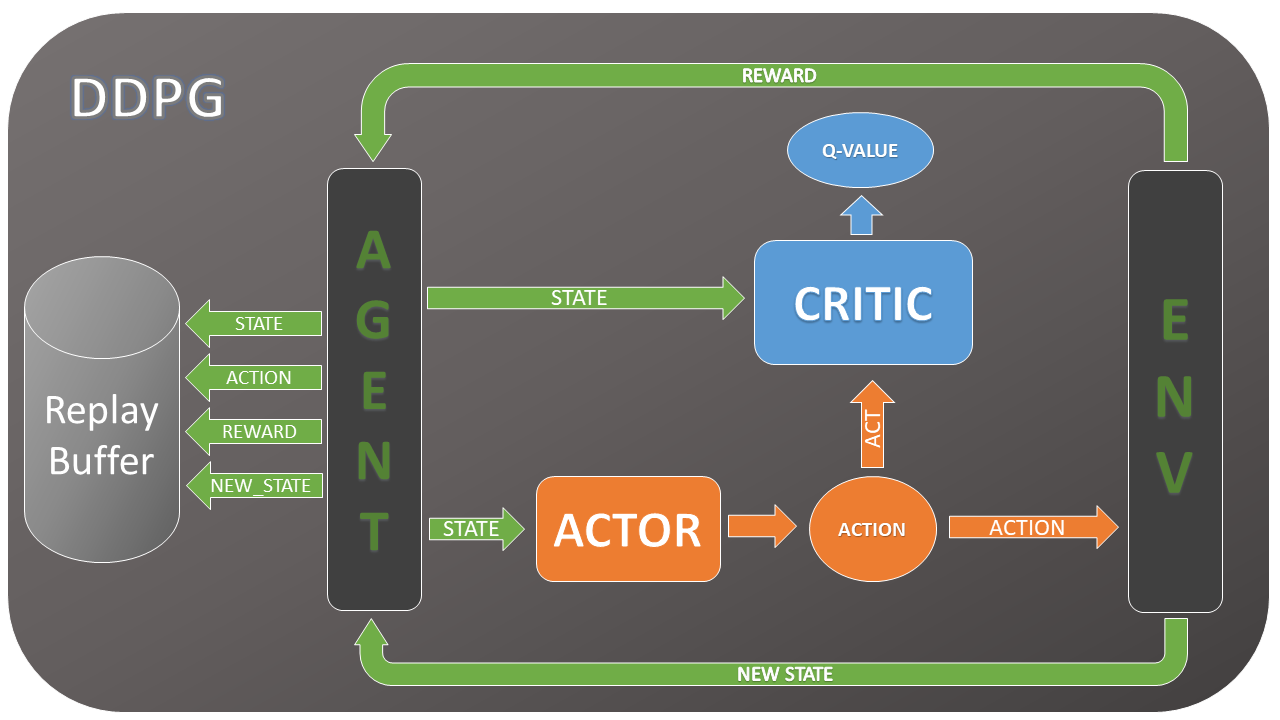
\includegraphics[width=1.\textwidth, height=.36\textheight]{pictures/ddpg_schema}
\caption{ A visual representation of the DDPG architecture. The Q-values is used only at training time.}
\end{figure}



\begin{algorithm}
	\caption{Deep Deterministic Policy Gradient}
	\label{algo:DDPG}
	\begin{algorithmic}[]
		\State Input: initial policy parameters $\theta$, Q-function parameters $\phi$, empty replay buffer {D}. 
		\State Set target parameters equal to main parameters $\theta_{targ} \leftarrow \theta $, $\phi_{targ} \leftarrow \phi $  
         \For{episode=1,M}
          
			\State Observe state s and select action $a=\operatorname{clip}\left(\mu_{\theta}(s)+\epsilon, a_{L o w}, a_{H i g h}\right),$ where $\epsilon \sim \mathcal{N}$
            \State Execute $a$ in the environment
            \State Observe next state {s'},reward {r}, and done signal {d} to indicate whether {s'} is terminal 
            \State Store (s,a,r,s',d) in replay buffer D
            \State \textbf{If} s' is terminal state reset the environment state.
            \If{it's time to update}
            	\For{however many updates}
                	\State Randomly sample a batch of transitions, $B={(s,a,r,s',d)}$ from D
                    \State Compute targets
                    \State $y\left(r, s^{\prime}, d\right)=r+\gamma(1-d) Q_{\phi_{\text {targ }}}\left(s^{\prime}, \mu_{\theta_{\text {targ }}}\left(s^{\prime}\right)\right)$
                    \State Update Q-function by one step of gradient descent using
                     \State $\nabla_{\phi} \frac{1}{|B|} \sum_{\left(s, a, r, s^{\prime}, d\right) \in B}\left(Q_{\phi}(s, a)-y\left(r, s^{\prime}, d\right)\right)^{2}$
                    \State update policy by one step of gradient ascent using:
                    \State $\nabla_{\theta} \frac{1}{|B|} \sum_{s \in B} Q_{\phi}\left(s, \mu_{\theta}(s)\right)$
                    \State Update target networks with
                    \State $\phi_{\mathrm{targ}} \leftarrow \rho \phi_{\mathrm{targ}}+(1-\rho) \phi$
					\State $\theta_{\mathrm{targ}} \leftarrow \rho \theta_{\mathrm{targ}}+(1-\rho) \theta$
                    	
                \EndFor
            \EndIf       
      \EndFor                         
	\end{algorithmic}
\end{algorithm}




\clearemptydoublepage
% Chapter 5

\chapter{Model Based Reinforcement Learning} % Main chapter title

\label{Chapter5} 
In this chapter we focus on Model Based approach, explaining how in works theoretically, why is useful and how could use it to create better agents. Then we present some  significant proposal from the literature and lastly we introduce the model used for this thesis. 


% Method name
\newcommand{\method}{PlaNet}
\newcommand{\fullmethod}{Deep Planning Network }
\newcommand{\Foruno}{\\  $\mathbf{\textbf{for } }$  }
\newcommand{\Fordue}{\\ \tab{} $\mathbf{\textbf{for } }$  }
\newcommand{\Fortre}{\\ \tab{} \tab{} $\mathbf{\textbf{for } }$  }
%\newcommand\tab[1][1cm]{\hspace*{#1}}
%\newcommand\Doubletab[1][2cm]{\hspace*{#1}}

\section{Model Based Reinforcement Learning}
% intro presa da https://arxiv.org/pdf/1903.11981.pdf

As we said in chapter \ref{Chapter3} in the reinforcement setting, there is an environment in a specific state $s_t$ that receives an action $a_t$ from an agent. 
After receiving this action, the environment update its state using the transition probability function $s_{t+1} = f\left(s_{t}, a_{t}\right)$
and calculates also the correspective reward $r_{t+1}=r\left(s_{t}, a_{t}\right).$
The agent takes the new observation from the environment and uses that to choose the next action to take $a_t=\pi(a_t|o_t)$.
Recall that in an MDP on observation correspond to the state, so $o_t = s_t$, while in an POMDP the observation is derivative of the state, so $o_t=o(s_t)$.

In the model-free setting, the agent will learn a policy that returns the best action directly to take in that state in order to maximize the expected cumulative reward.
In the model-based setting, instead, the agent will learn to model the dynamics of the environment (forward model) by approximating the transition function and the reward function.
So in case of MDP the model could be:
$ s_{t+1} = f_\theta (s_t,a_t).$
Instead if the environment is a POMDP the model need to use also the old observation and actions, in order to predict a new one.
$ o_{t+1} = f_\theta(o_0,a_0,...,o_t, a_t)$

Once the agent is able to approximate the environment in its head, it is also able to  simulate actions and predicts the possible consequences.

To be more specific, the agent plan a sequence of H (that stands for Horizon) actions $ \left\{ a_{t},\ldots, a_{t+H}\right\}$, and then unroll the learned model H step into the future based on those actions.
Now the agent can compute the objective function. 
$ G\left(a_{t}, \ldots, a_{t+H}\right) =\mathbb{E}\left[\sum_{\tau=t}^{t+H} r\left(o_{\tau}, a_{\tau}\right)\right] $ to evaluate the current plan and performs some sort of optimization to find the best possible plan (often a genetic algorithm is used to this purpose)
$ a_{t}, \ldots, a_{t+H} =\arg \max G\left(a_{t}, \ldots, a_{t+H}\right) $.
This process is called  \textbf{trajectory optimization}.


\section{Planet}
Planet is a new algorithm published in 2019 from the research team in Google AI \cite{hafner2019learning}.
In this paper, the agent is able to learn environment dynamics only through the observation and then can use this model to plan what action to take for each step.
In order to achieve this task, the agent must solve three problems:

\begin{enumerate}
\item understanding the observation: capture the useful information contained in each frame and maintain them in memory
\item understanding the environment dynamics: be able to predict the next observation and the next reward having only the current observation and the current action as input
\item using its prediction to plan what action to take.
\end{enumerate}

\subsection{RSSM}
Since the planning requires a considerable amount of predictions at every time step, the researchers decided to work in latent space.
In other words, they do not use the entire frame to predict the next one, but they encode all the information in a vector obtained from neural networks, called latent vector. 
This advantage in terms of computational cost leads to a disadvantage for the agent that now has two jobs: first, it has to build a visual understanding of the environment and second, it has to find a way to solve the task.
To be more specific, they use a convolutional neural network to capture all the spatial information from the image, and a GRU network  (a simplified version of LSTM) to capture the temporal information across different time steps.
Then they use both information to create the latent vector.

Now it is time to enter in technical details:
We now considering sequences like $\left\{o_{t}, a_{t}, r_{t}\right\}_{t=1}^{T}$ where the index $t$ is used for the time step, $o_t$ is the environment observation for the current time step, $a_t$ and $r_t$ the current action and reward.
The Planet model is composed of three sub models:
\begin{align*}
\text { Transition model: } & s_{t} \sim p\left(s_{t} \mid s_{t-1}, a_{t-1}\right) \\
\text { Observation model: } & o_{t} \sim p\left(o_{t} \mid s_{t}\right) \\
\text { Reward model: } & r_{t} \sim p\left(r_{t} \mid s_{t}\right)
\end{align*}
The transition model has the job of produce the current latent state by using the previous latent state and the current action.
Then the observation model and the reward model will use it to reconstruct the observation and predict the reward obtained by the execution of $a_{t}$  in $s_{t}$. 

The \textbf{observation model} is Gaussian with a mean parameterized by a deconvolutional neural network and identity covariance.
The \textbf{reward model} is a scalar Gaussian with a mean parameterized by a feed-forward neural network and unit variance.
In both cases, the loss is calculated through mean square error.
The \textbf{transition model} can be viewed as a sequential VAE that is a convolutional variational autoencoder that receive in input an observation $o_t$ and an action $a_t$.
The aim of the encoder is to learn an approximation of the state posterior $q\left( s_{1:T} \mid o_{1:T}, a_{1:T}   \right) $ from past observation and actions. 
This state posterior will contain all the useful information about the current state to allow the decoder (introduced above as the observation model) to uses this state $s_t$ to reconstruct the observation $o_t$ completely.
When it produces the current posterior state, it needs to use also the information of the precedent state that is served as input in addition to the observation and action, and this is why it is called \textit{recurrent} VAE.
So the transition model approximate the true state posterior with $\prod_{t=1}^{T} q\left(s_{t} \mid s_{t-1}, a_{t-1}, o_{t}\right)$.
We can find the true parameters of this Gaussian at training time because we have all the information necessary to calculate the loss value througth mean squared error. 
Another important point is that at training time we can always sample a batch of transitions from the experience replay and  provide the current observation for each time step. 
At inference time instead, we only have the observation for the current step, but if we want to predict the posterior states of different steps in the future, we cannot provide the respective observation.

Intuitively if we ask the model to predict the next observations, it cannot require it as input.
For this reason we use this model at training time to find the correct parameter of the posterior state and in inference time we use another model that not use the information about the current observation $o_t$ but  it only require $s_{t-1}$ and $a_{t-1}$ $p(s_t | s_{t-1}, a_{t-1})$.
This new model $p$ is trained to stay close to $q$ via kl-divergence.
$KL\left[ q\left(s_{t} \mid s_{t-1}, a_{t-1}, o_{t}\right) || p\left(s_{t} \mid s_{t-1}, a_{t-1}\right)  \right]$.

Unfortunately, the only $s_{t-1}$ is not enough to maintain in memory all the useful information.
The form of stochastic transition, in fact, not able to maintain information across multiple steps.
For this reason, they also provide the model with a sequence of activation vectors $\left( h_t \right) ^{T}_{t=1}$ from a GRU network.
Combining these two methods, they create a new model called \textbf{Recurrent State-Space Model (RSSM)}.
In RSSM, the internal state is composed of two parts: a stochastic one named $s_t$ (sampled from a Gaussian) and a determinist part $h_t$ (sampled from GRU).
The final model is similar to the previous one:
\begin{align*}
\text { Deterministic state model: } & h_{t} = f\left(h_{t-1} , s_{t-1}, a_{t-1}\right) \\
\text { Stocastic state  model: } & s_{t} \sim p\left(s_{t} \mid h_{t}\right)  \text {*}\\
\text { Observation model: } & o_{t} \sim p\left(o_{t} \mid h_{t}, s_{t}\right) \\
\text { Reward model: } & r_{t} \sim p\left(r_{t} \mid h_{t}, s_{t}\right)\\
\text{*the information over action is already encoded in h}
\end{align*}
Now at inference time, the model can rely only on $h_t$.

Before moving on to the next paragraph, I left a quick visual recap of the Planet model.

\begin{figure}[H]
\centering
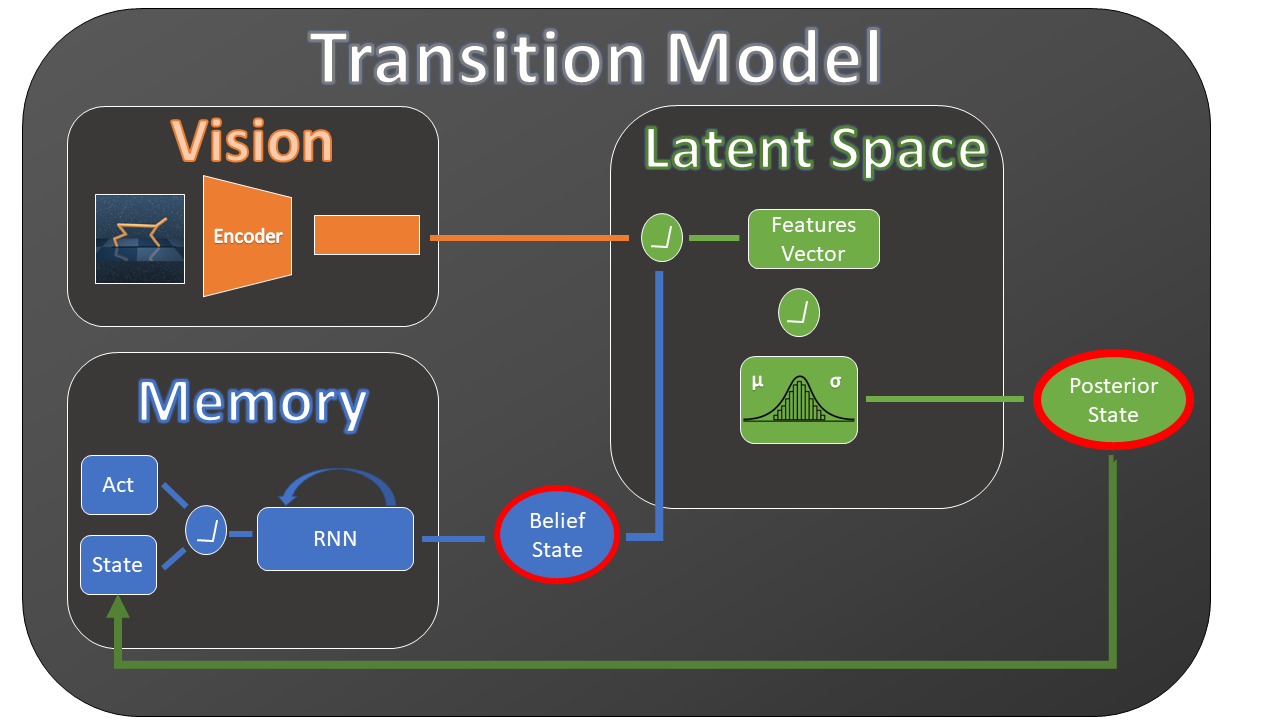
\includegraphics[width=1.\textwidth, height=.4\textheight]{pictures/planet_schema}
\caption{ The transition model at inference time. The current frame is encoded and the RNN produces the current Belief State encoding the current action and the previous posterior state. The current encoded observation and the Belief State are combined to produce the Features Vector from where the posterior Gaussian parameters are produced. In the last step, the current Posterior state is sampled from the Gaussian.}
\end{figure}

\begin{figure}[H]
\centering
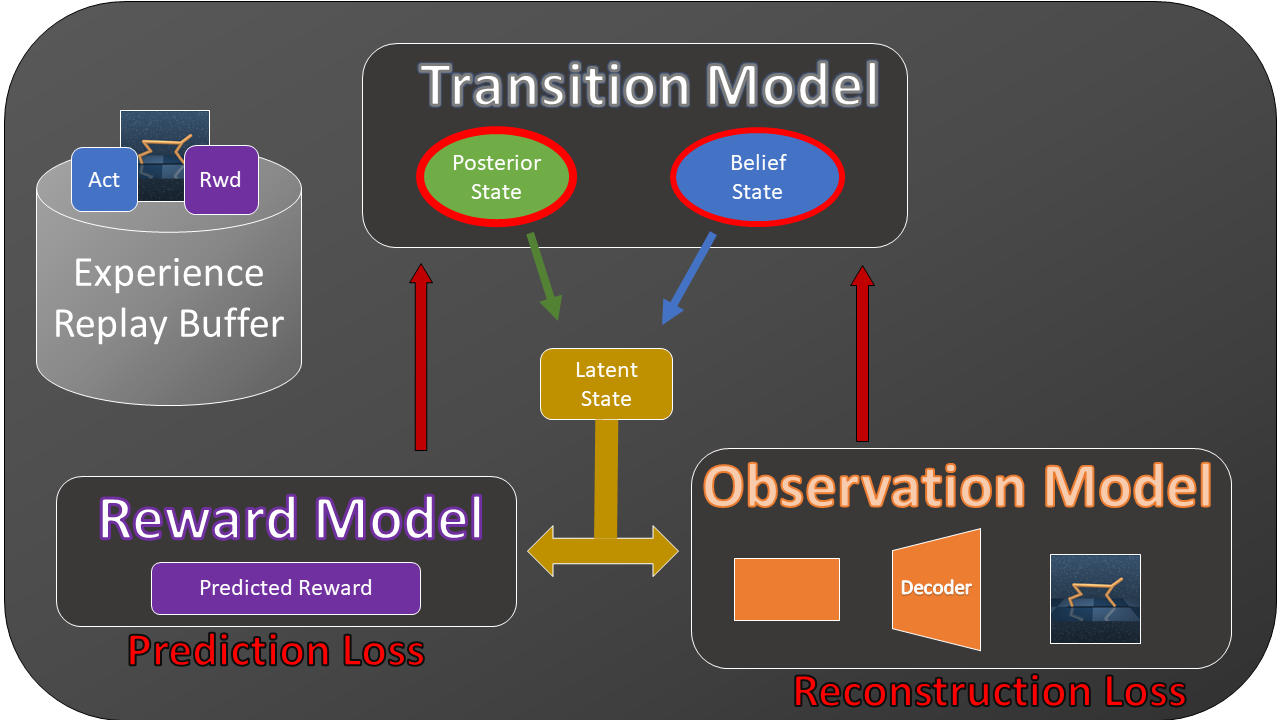
\includegraphics[width=1.\textwidth, height=.4\textheight]{pictures/planet_loss}
\caption{ The current Latent State is produced by the combination of both Belief State and Posterior State. This Latent State is then used by the Reward Model to predict the reward and by the Observation Model to reconstruct the current observation. With these two results we can calculate the mean squared error (by sampling the original result from the buffer) and backpropagate the loss to train the transition model. }
\end{figure}

\begin{figure}[H]
\centering
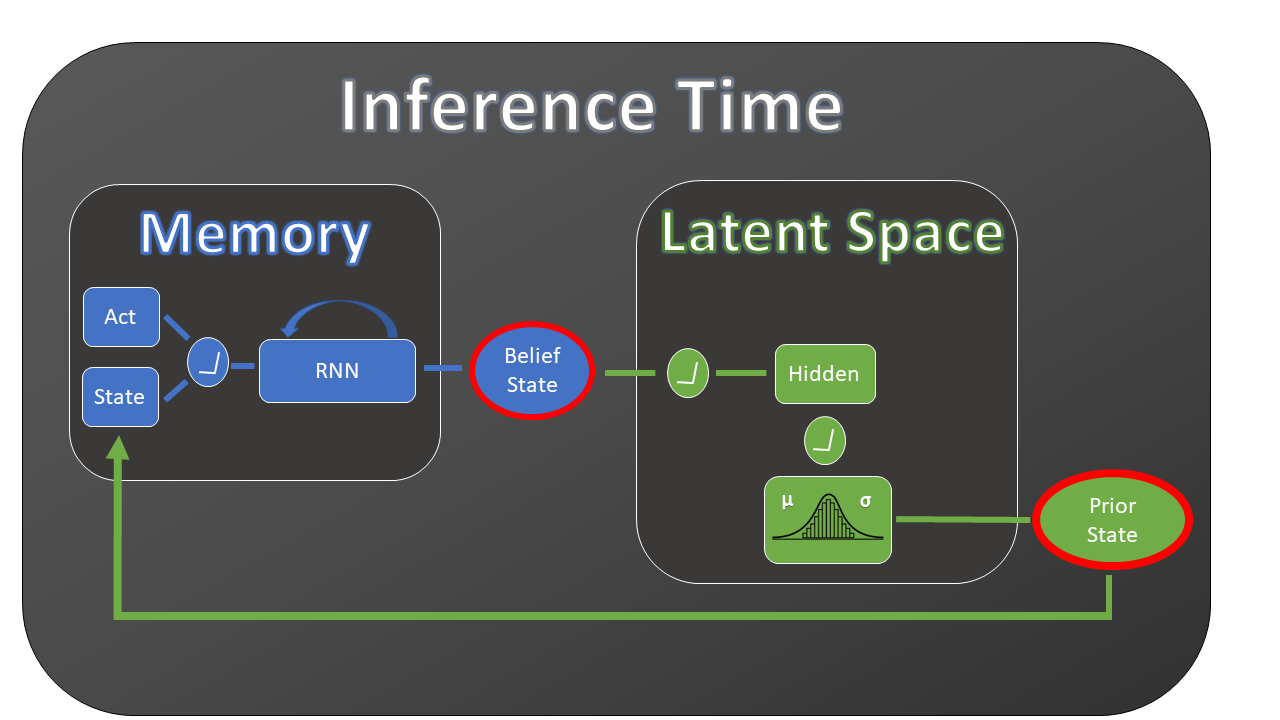
\includegraphics[width=1.\textwidth, height=.4\textheight]{pictures/planet_inference}
\caption{ At inference time we have no more the experience replay buffer that provide us the observation for each step. We only have the observation for the current step provided by the environment and we have to predict the next for many steps ahead.}
\end{figure}
\begin{figure}[H]
\centering
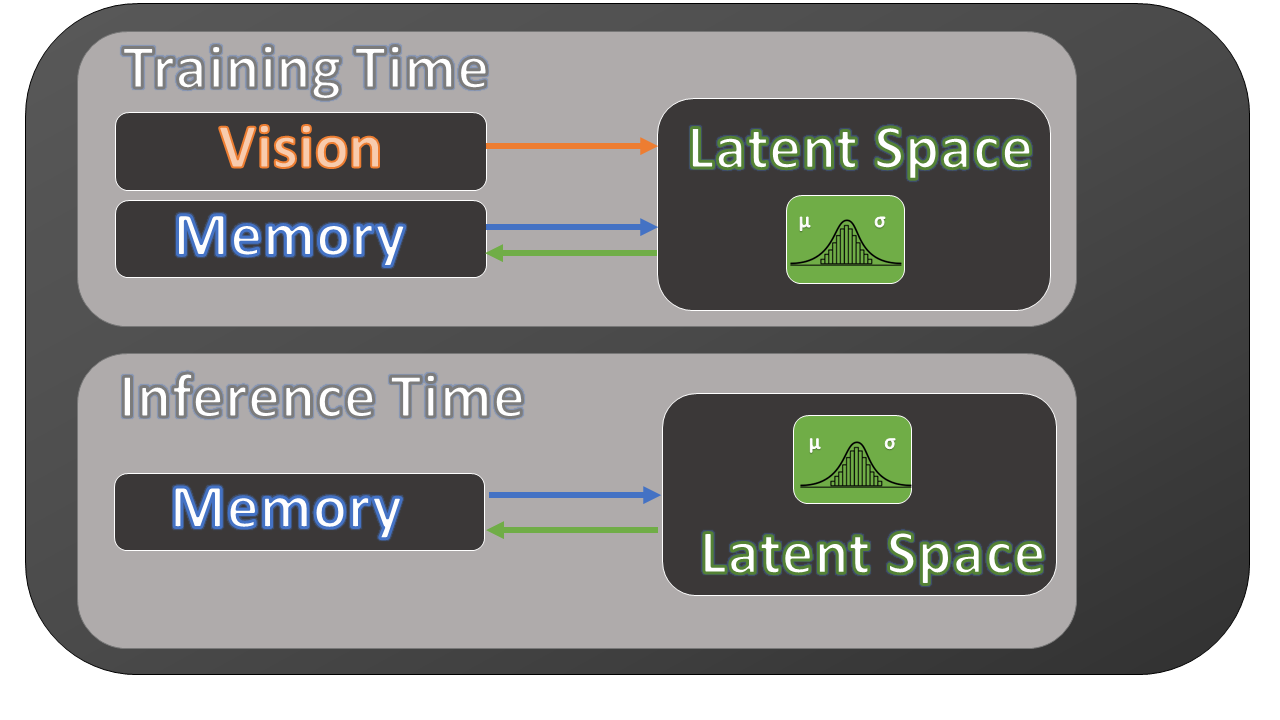
\includegraphics[width=1.\textwidth, height=.4\textheight]{pictures/planet_train_infer}
\caption{ We can reuse the Memory model (RNN) used for the transition model at training time but we need to retrain the Gaussian model. We need a way to obtain the same parameters  used by the model at training time. }
\end{figure}
\begin{figure}[H]
\centering
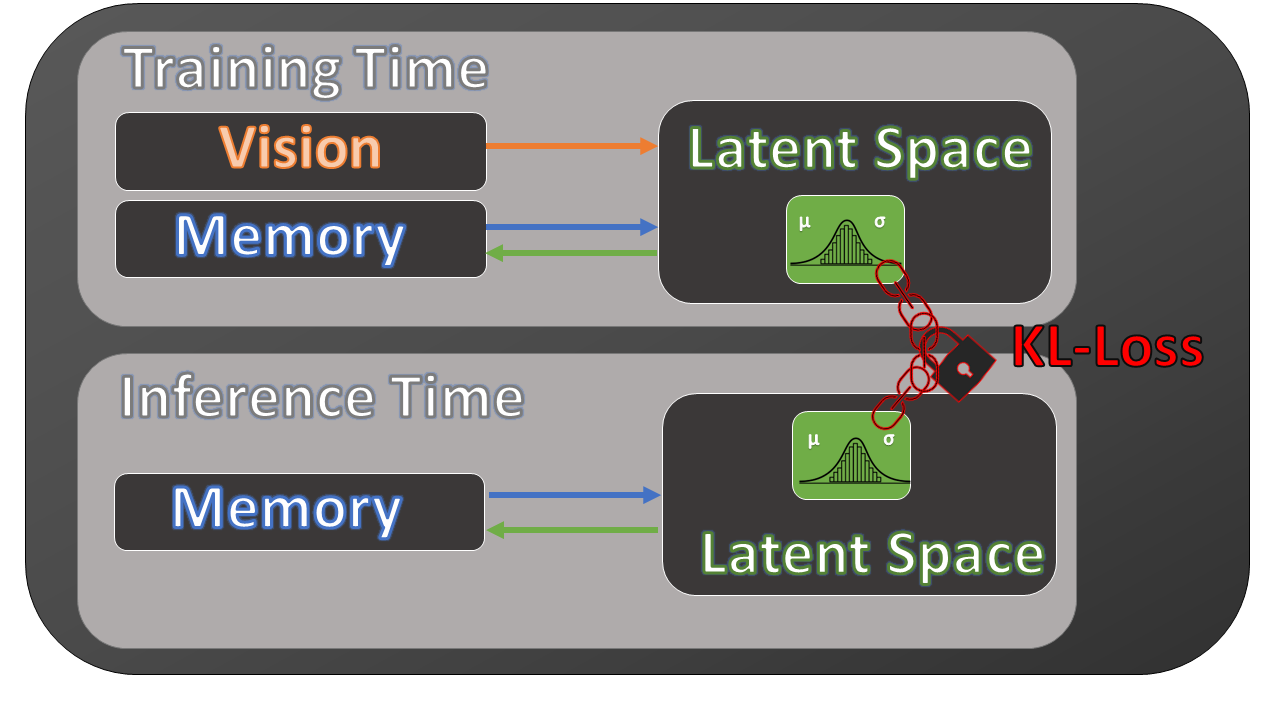
\includegraphics[width=1.\textwidth, height=.4\textheight]{pictures/kl_loss_chain}
\caption{ The loss indicates how much information we lost by approximate the Gaussian produced at training time with the one used at inference time. }
\end{figure}


\subsection{Planning}
Now it's time to use the model for planning. 
Even if the model that predicts the future is robust, a perfect prediction over the entire episode is unrealistic. 
The more we try to predict in the future, the more the prediction error will accumulate, and the more the prediction will diverge to reality.
For this reason, the planning is computed over a short horizon $H$.
They used the Cross-Entropy Method to perform trajectory optimization. It is a robust method and is proved to be capable of solving all the tested environments when true dynamics are given.
Initially, the actions vector, that contains all the actions from the current time step $t$ to the planning horizon $H$, is sampled from a Gaussian with zero mean and unit variance $a_{t: t+H} \sim \operatorname{Normal}\left(\mu_{t: t+H}, \sigma_{t: t+H}^{2} \right)$.
For each generation, $J$ candidates action vectors are sampled and evaluated using the transition model and the reward model.
The evaluation is base on how much reward is produced over the time steps.
For each generation, the parameters update of the Gaussian is calculated over the top k elements of the candidates' population.
Even if the planner has produced a plan over H time steps when the first action is executed, and the new observation is received, the planning process is replicated and adapted to the latest information.
In other words, the planning is computed at every step, and only the first planned action is used. 
It is still necessary to planning over a horizon longer than one because that will lead to local optima.

\section{Cross Entropy Method}
%https://arxiv.org/pdf/1810.01222.pdf

The Cross-entropy (CE) method is an EDA (Estimation of Distribution Algorithms) used in many optimization problems of the form:
$$w^{*}=\arg \max _{w} S(w)$$
where w is a set o weight, and S is a generic objective function of w. 
The EDA is a specific family of Genetic Algorithms that
does not work with a single solution but distributions of possible solutions represented with a covariance matrix $ \Sigma $.
This covariance matrix is used to defines a multivariate Gaussian function and for sampling the population for the next iteration.
Iterations after iterations, the ellipsoid defined by $\Sigma$ is moved to the top part of the hill corresponding to the local optimum $\theta^*$.
A each time step the entire population is sampled from the current parameters of the distributions. 
Next So all the new individuals are evaluated according to the problem-dependent fitness function $(f_i)_{i=1,...,\lambda}$.
Then the top $K_e$ individuals $(z_i)_{i=1,...,K_e}$ (called \textbf{elites} or \textbf{candidates}) are used to update the distribution parameters (the new mean and variance are calculated over the elites).

\begin{align*} 
\mu_{n e w} &=\sum_{i=1}^{K_{e}} \lambda_{i} z_{i} \\ \Sigma_{n e w} &=\sum_{i=1}^{K_{e}} \lambda_{i}\left(z_{i}-\mu_{o l d}\right)\left(z_{i}-\mu_{o l d}\right)^{T}+\epsilon \mathcal{I}, 
\end{align*}

Notice that $(\lambda_i)_{i=1,...,K_e}$ are weights assigned to each individual (a common choice is $\lambda_i = \frac{1}{K_e}$.
Usually some extra variance $\epsilon$ is added in order to prevent premature convergence.
To be more specific some Gaussian noise is added to each individual $x_i$ that is sampled from the current covariance matrix $\Sigma$.

\begin{algorithm}[h!]
\textbf{Input:}
\begin{tabular}[t]{l @{\hspace{.5em}} l}
$H$ & Planning horizon distance \\
$I$ & Optimization iterations \\
$J$ & Candidates per iteration \\
$K$ & Number of top candidates to fit \\
\end{tabular}%
\begin{tabular}[t]{l @{\hspace{.5em}} l}
$q(s_t|o_{\leq t},a_{<t})$ & Current state belief \\
$p(s_t|s_{t-1},a_{t-1})$ & Transition model \\
$p(r_t|s_t)$ & Reward model \\
\end{tabular}% 
\\ Initialize factorized belief over action sequences $q\left(a_{t: t+H}\right) \leftarrow \operatorname{Normal}(0, \mathbb{I})$. \;
\Foruno{optimization iteration $i=1..I$}{
  \\\tab{ \textit{// Evaluate $J$ action sequences from the current belief.}}
  \Fordue{candidate action sequence $j=1..J$}{
     \\\Doubletab{ $a^{(j)}_{t:t+H}\sim q(a_{t:t+H})$ \;}
     \\\Doubletab{ $s^{(j)}_{t:t+H+1}\sim
        q(s_t|o_{1:t},a_{1:t-1})
        \prod_{\tau=t+1}^{t+H+1}p(s_\tau|s_{\tau-1},a^{(j)}_{\tau-1})$ \;}
      \\\Doubletab{ $R^{(j)}=\sum_{\tau=t+1}^{t+H+1}E{p(r_\tau|s^{(j)}_\tau)}$ \;}
  }
  \\\tab{\textit{//Re-fit belief to the $K$ best action sequences}.}
  \\\tab{$\mathcal{K}\leftarrow\mathrm{argsort}(\{R^{(j)}\}_{j=1}^J)_{1:K}$ \;}
  \\\tab{$\mu_{t:t+H}=\frac{1}{K}\sum_{k\in\mathcal{K}} a_{t:t+H}^{(k)}, \quad
  \sigma_{t:t+H}=\frac{1}{K-1}\sum_{k\in\mathcal{K}}|a_{t:t+H}^{(k)}-\mu_{t:t+H}|$. \;}
  \\\tab{$q(a_{t:t+H})\leftarrow\operatorname{Normal}(\mu_{t:t+H},\sigma_{t:t+H}^2\mathbb{I})$ \;}
}
\\\Return{first action mean $\mu_t$.}
\caption{Latent planning with CEM}
\label{alg:planner}
\end{algorithm}

\subsection{Algorithm}
Finally, we have all the information to describe the entire flow of the Planet algorithm.
Initially, some random episodes ( every action is chosen randomly) are executed in order to collect some data in the experience replay buffer.
Then the main training loop, which is composed of two procedures called model fitting and data collection, can begin.
\textbf{The model fitting procedure} consists of sampling sequence chunks from the buffer experience and train the model.
\textbf{The data collection procedure} consists of using the model to solve an episode and collect new data. 
Since the aim of this procedure is not to solve the environment but collect new data, random Gaussian noise is added over the action before it is executed to have a better exploration of the environment.
This noise is not used when we want to use/evaluate the model.





This iterative approach allows the model to collect also the data that is not obtainable from the random init episodes.



\begin{algorithm}
\textbf{Input:}
{\\\hspace{-3.6em}\small
\begin{tabular}[t]{l @{\hspace{.5em}} l}%
$R$ & Action repeat \\
$S$ & Seed episodes \\
$C$ & Collect interval \\
$B$ & Batch size \\
$L$ & Chunk length \\
$\alpha$ & Learning rate \\
\end{tabular}\hspace{-0.5em}%
\begin{tabular}[t]{l @{\hspace{.5em}} l}%
$p(s_t|s_{t-1},a_{t-1})$ & Transition model \\
$p(o_t|s_t)$ & Observation model \\
$p(r_t|s_t)$ & Reward model \\
$q(s_t|o_{\leq t},a_{<t})$ & Encoder \\
$p(\epsilon)$ & Exploration noise \\
\end{tabular}%
}
\\
\\Initialize dataset $\mathcal{D}$ with $S$ random seed episodes.
\\Initialize model parameters $\theta$ randomly. \;
\\
\textbf{while}{(not converged)}{
	 \\
	\tab{// Model fitting}
	\Fordue{update step $s=1..C$}{ 
    \\\Doubletab{Draw sequence chunks $\{(o_t,a_t,r_t)_{t=k}^{L+k}\}_{i=1}^B\sim\mathcal{D}$ uniformly at random} \Doubletab{ from the dataset.}
   \\\Doubletab{ Compute loss $\mathcal{L}(\theta)$ . \;}
    \\\Doubletab{Update model parameters $\theta\leftarrow\theta-\alpha\nabla_\theta\mathcal{L}(\theta)$. \;}
  }
  \\
  \\\tab{// Data Collection}
  \\\tab{$o_1\leftarrow\texttt{env.reset()}$ \;}
  \Fordue{time step $t=1 . .\left\lceil\frac{T}{R}\right\rceil \mathbf{d o}$}{\\
    \Doubletab{ Infer belief over current state $q(s_t|o_{\leq t},a_{<t})$ from the history. \;}
    \Doubletab{$a_t\leftarrow\texttt{planner(}q(s_t|o_{\leq t},a_{<t}),p\texttt{)}$  see \ref{alg:planner} for details \;} 
    \\\Doubletab{Add exploration noise $\epsilon\sim p(\epsilon)$ to the action. \;}
    \Fortre{action repeat $k=1..R$}{
      \\\Doubletab{\tab{$r_t^k,o_{t+1}^k\leftarrow\texttt{env.step(}a_t\texttt{)}$ \;}}
    }
    \\\Doubletab{$r_t,o_{t+1} \leftarrow \sum_{k=1}^R r_t^k, o_{t+1}^R$ \;}
  }
  \\\tab{$\mathcal{D}\leftarrow\mathcal{D}\cup\{(o_t,a_t,r_t)_{t=1}^T\}$ \;}
  \\
}
%\vspace{-2ex}
\caption{\fullmethod (\method)}
\label{alg:agent}
\end{algorithm}




\clearemptydoublepage
% Chapter 6

\chapter{Experiments} % Main chapter title

\label{Chapter6} % For referencing the chapter elsewhere, use \ref{Chapter1} 
In this chapter, we introduce the benchmark environments used to compute all the tests. We show the results obtained, the proposal for improvement, and a comparison between the model-free approach represented by the DDPG algorithm and the model-based approach represented by PlaNet.

\section{DeepMind Control Suite}
All the experiments are based on Deepmind Control Suite \cite{tassa2018deepmind}.
The control suite is a set of continuous control tasks that are built for benchmarking reinforcement learning agents. The main focus is on continuous control. The environments can provide a fully observable state (a feature vectors) and a partially observable state (a scene) frame. All the environments are written in Python and powered by the MuJoCo physics engine. A visual representation of the main environments available in the Deepmind control suite is shown below.


\begin{figure}[h]
\centering
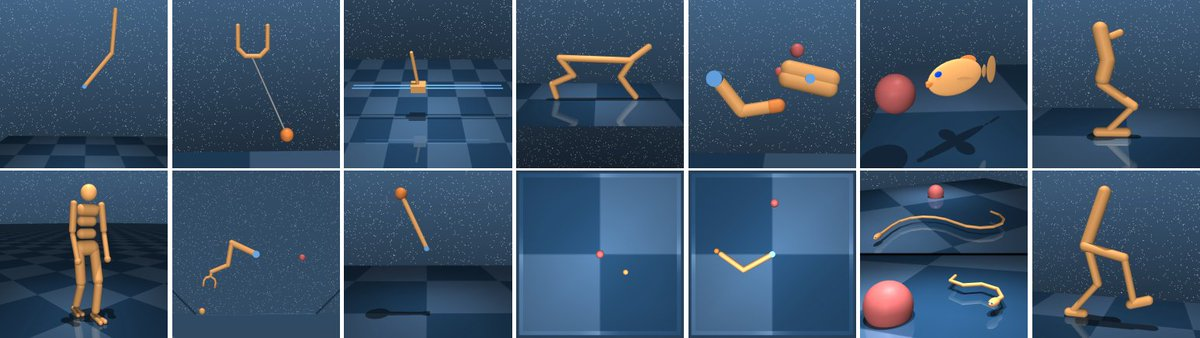
\includegraphics[width=1.0\textwidth]{pictures/dm_control}
                  \caption{. Top: Acrobot, Ball-in-cup, Cart-pole, Cheetah, Finger, Fish, Hopper.
Bottom: Humanoid, Manipulator, Pendulum, Point-mass, Reacher, Swimmer (6 and 15 links), Walker.}
            \end{figure}
The principal environment that we choose to experiment is the half-cheetah that is a very common choice. 

In this environment, the agent should move forward as quickly as possible with a cheetah like body that is constrained to the plane. The reward is linearly proportional to a maximum of $10_{\mathrm{m} / \mathrm{s}}$ i.e. $r(v)=\max (0, \min (v / 10,1))$.
A vector of 18 dimensions describes each state while the actions are represented with a vector of 6 dimensions.

In addition to this environment, we have chosen three more to test the consistency of the tests.

The other environments are:
\begin{itemize}
\item Cart-pole (task: swing-up): The classic cart-pole swing-up task. The agent must balance a pole attached to a cart by applying forces to the cart alone. The pole starts each episode hanging upside-down.

\item Walker (task: walk): Agent should move forward as quickly as possible with a bipedal walker constrained to the plane without falling or pitching the torso too far forward or backward.

\item Reacher: (mode: easy): The simple two-link planar reacher with a randomized target location. The reward is one when the end effector penetrates the target sphere.
\end{itemize}



\section{Model Free experiments }
We choose DDPG as a model-free algorithm for the experiments since it is compatible with environments with continuous action spaces. 
It also guarantees a good sample efficiency thanks to the buffer experience replay.

In this experiment we want to find out what level of performances a DDPG agent can reach with a million of steps.
We start from the original DDPG paper \cite{lillicrap2015continuous} but when it was released, the Deepmind control suite did not exist yet.
All the benchmarks in that paper, for the cheetah problem, are based on another suite provided by Open Ai called Gym.
Even if both the environments from Open Ai and Deepmind are based on the same physic engine (MuJoCo) and representing the same problem (the cheetah problem), they have significant differences that require a different set of parameters. 
All the parameters provided in the original paper are based on the Open Ai Gym version.

We addressed this problem in two phases.
At first, we precisely replicated the original paper model with the Open Ai Gym environment to be sure to have a solid implementation. 
We tried to retrain our model in the Deepmind Control Suite environment without the tuning process, without success. 
The DDPG algorithm proved to be very susceptible to the parameters. 
We tried another approach based on the Deepmind Control Suite paper in which the author explained how they trained the DDPG algorithm in their environments, and we are successfully reproduced their results.

In our implementation, we used Adam (\cite{kingma2014adam}) for learning the neural network parameters with a learning rate of $10^{-4}$ for both the actor and critic networks.
For the critic network, we included a $L_2$ weight decay of 0.002 and used a discount factor of $\gamma = 0.99$. 
We used both a soft update (with $\tau = 0.001$) and a hard update (every 100 steps) for the target networks. 
The activation function is the Relu for all the hidden layers and the Tanh for the actor final output layer.
After the activation, I apply batch normalization.
In the final layer (for both actor and critic networks) both the weight and bias are initialized from uniform distribution $\left[-3 \times 10^{-3}, 3 \times 10^{-3}\right]$.
The hidden layers instead are initialized from uniform distributions $\left[-\frac{1}{\sqrt{f}}, \frac{1}{\sqrt{f}}\right]$ where $f$ is the fan-in of the layer.
The actor-network is composed of 3 hidden layers with respectively [128,300,400] units.
Only for the actor-network, the gradients are clipped at [-1,1].
The critic-network is composed of two separate input layers (one for the action with 256 units and two for the state with 128,256 units). 
Then the two activations are summed together and passed to another 2 hidden layers with 300 and 400 units.
Lastly we used an Ornstein-Uhlenbeck process to produce the noise for the exploration. The parameters are: $\theta = 0.15$ and $\sigma = 0.3$.
We do not perform warm-up episodes to prefill the buffer before training.

The results of our experiments are shown below.
\begin{figure}[H]
\centering
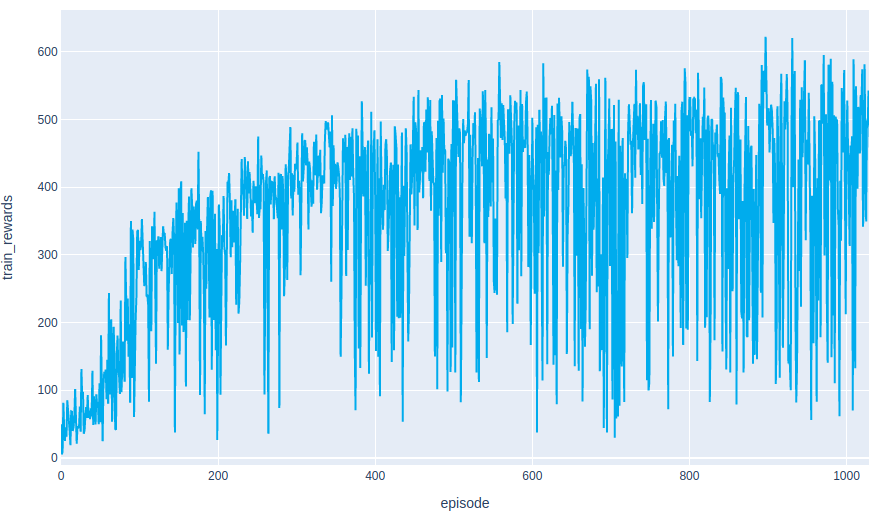
\includegraphics[width=1.\textwidth, height=.35\textheight]{pictures/ddpg_train_rew_with_feature_state}
\caption{ Results of the training of the DDPG algorithm on DeepMind Control Suite Ceetah environment.}
\end{figure}
Every episode corresponds to 1000 steps, and the training consists of 1 million steps.
During the training, at every action is added a gaussian noise.
To understand the real performance of the model, a test without noise is computed every 100 episodes.

\begin{figure}[H]
\centering
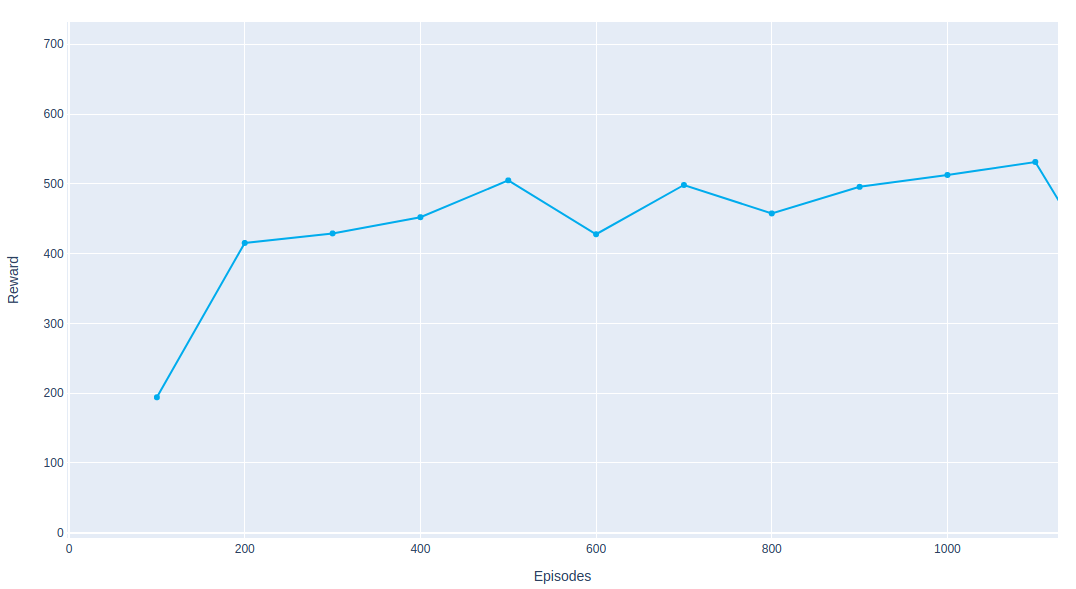
\includegraphics[width=.9\textwidth, height=.35\textheight]{pictures/ddpg_frame_as_input_test}
\caption{ Results of the test with the model trained with the DDPG algorithm from feature vectors.}
\end{figure}
This result is consistent with the performance published by the Deepmind Control Suite authors \cite{tassa2018deepmind}.

\begin{figure}[H]
\centering
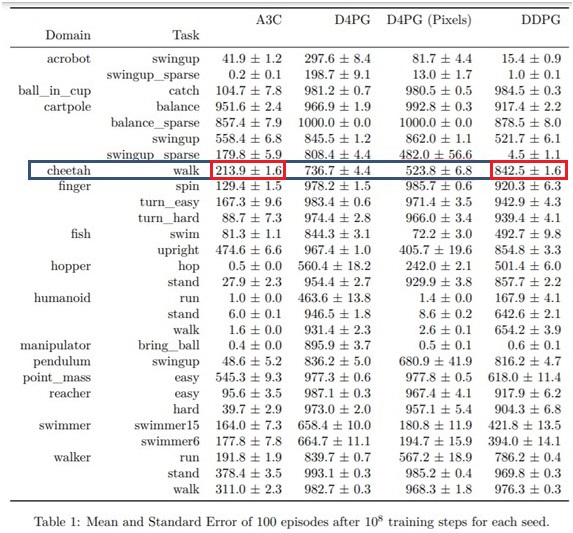
\includegraphics[width=.75 \textwidth, height=.45 \textheight]{pictures/dmcs_ddpg_vs_a3c}
\caption{ Result of the experiments from the Deepmind Control Suite team \cite{tassa2018deepmind}.}
\end{figure}

As we can see from the image above our implementation outperform the A3C algorithm and reach a cumulative reward value of 500 after $10^6$ steps that is compatible with the $812.5$ obtained from the research team after $10^8$ steps.


After our experiments, we can say that the DDPG algorithm is proved to be very sensitive to the hyperparameters.
We notice that some parameters like the initialization of the layers, the learning rate are more impact respect to the others.




\section{Model Free experiments from frames}
The use of the features vectors requires a human expert's intervention. This can be a limitation and also a source of error in the construction of the environment.

In this experiment, we want to find out if the DDPG algorithm is capable of solving this task directly from the raw pixels and in that case, how much the difficult of the problem increase.

With this new formulation, the observation provided does not correspond to the real markovian state of the MDP.
The authors of the Deepmind Control Suite doesn't use the DDPG algorithm to solve this problem but switched to an advanced version of the algorithm called  Distributed Distributional Deterministic Policy Gradients (\textbf{D4PG}).
They showed that this version of the algorithm after $10^8$ steps, is able to learn a policy also in this condition, but is not capable of achieving the same performances of the experiments with features vector as input. 

\begin{figure}[H]
\centering
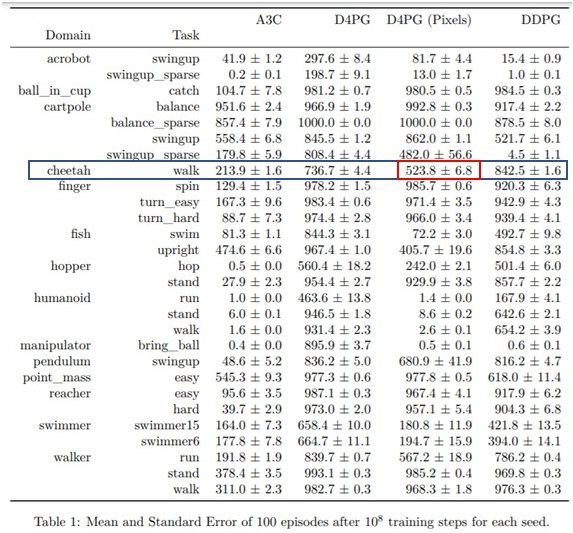
\includegraphics[width=.75 \textwidth, height=.45 \textheight]{pictures/dmcs_d4pg}
\caption{ Result of the Deepmind Control Suite team obtained with the D4PG algorithm\cite{tassa2018deepmind}.}
\end{figure}

We still tried to train a DDPG agent from raw pixels. 
As suggest in the original paper \cite{lillicrap2015continuous} we used the action repeats trick to enrich the information provided at each step. So at each step, the agent computes the same action 3 times. We have transformed the obtained 3 frames to grayscale, and we stacked them together the creating a new single input of 3 feature maps. The original version does not apply the grayscale conversion and provide an input of 9 feature maps. We notice anyway that this preprocessing step is very useful.
All the frames are downsampled to 64x64 pixels and normalized in a range between [0,1]. 
We added a new set of convolutional layers to the model to handle the frames high dimension.
We experimented with different approaches to network architecture.
Initially, I tried to create two convolutional networks, one for the actor and another for the critic but did not work well.
The best performance is obtained by weight-sharing of the convolutional network, as shown in the image below.

\begin{figure}[H]
\centering
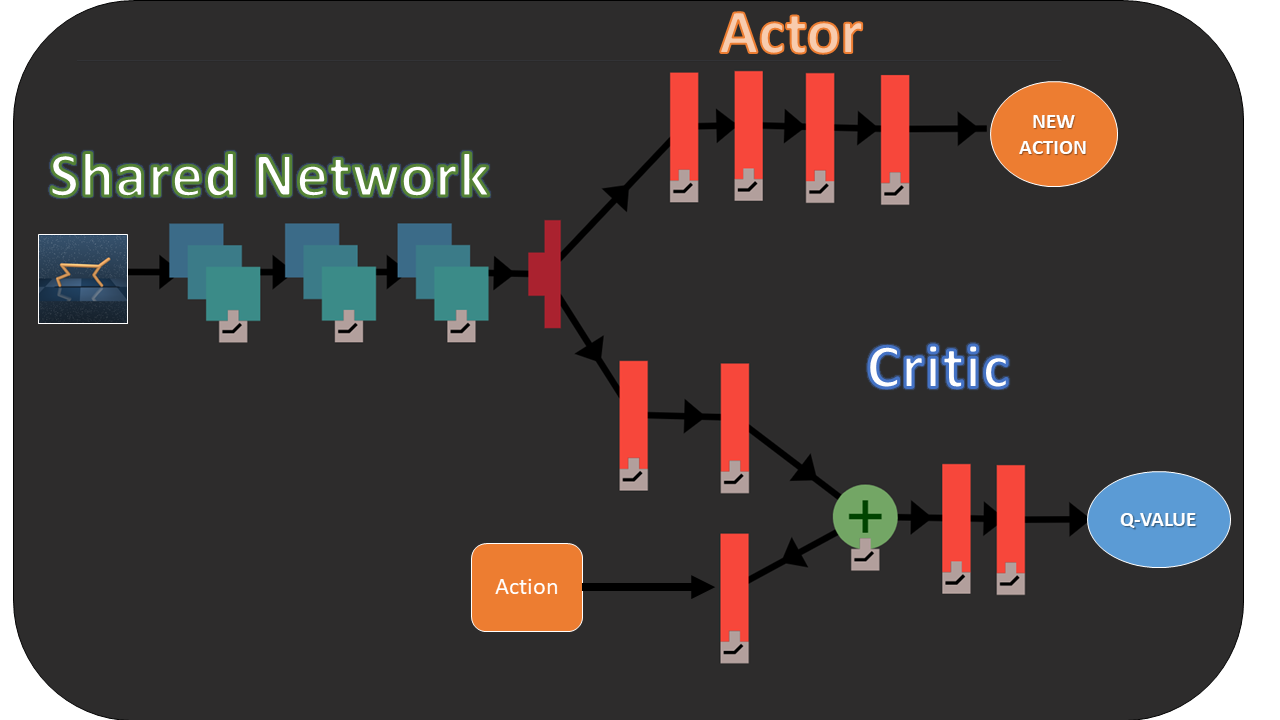
\includegraphics[width=1.\textwidth, height=.35\textheight]{pictures/ddpg_shared_net}
\caption{ Visual representation of the model architecture with the convolutional network shared between actor and critic.}
\end{figure}

Whenever the actor or the critic receives a frame as input, they call the shared convolutional network to encode the frames and return the corresponding features vector.
As suggested in \cite{tassa2018deepmind}, only the Critic network is allowed to update the shared network weights; in other words, the Actor gradients are truncated.
The shared network is composed of three layers, all with a kernel size of 3 x 3 with 32 channels (only the first layer with has also a stride of 2),  followed by two fully-connected layers with 200 and 50 neurons, with layer normalization.
All other parameters are the same as in the previous experiment, except the batch size is set to 256.

We stop the training after $10^6$ steps like all the other experiments. The results are shown below.

\begin{figure}[H]
\centering
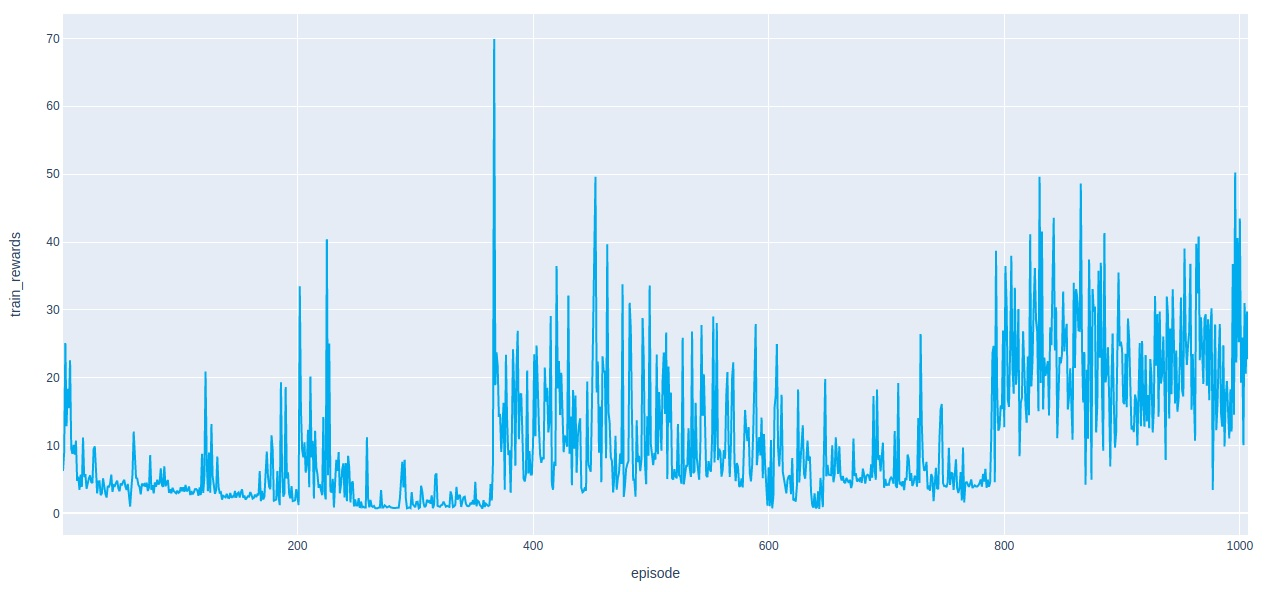
\includegraphics[width=1.\textwidth, height=.4\textheight]{pictures/ddpg_train_reward_with_frames_2}
\caption{ Result of training DDPG for the cheetah problem, after 1000 episodes using frames as input .}
\end{figure}

As we can see, after 1000 episodes (1 million steps), the agent is not able to reach significative performance. 
The training curve has risen slightly, indicating that full training would require several thousand more episodes.
Due to the limits of the computational budget is was not possible to train the network entirely.
%The test curve (obtained by using the same model at training time but without adding noise to the actions) confirms that after 1000 episodes, the training is just at most at the beginning phase, and the agent is not learning yet.

We suppose that the convolutional layers require a lot of transition before learning the useful pieces of information to capture from every image.
Until the convolutional layers are not trained, the policy can't learn.
We can clearly see how to learn from raw pixels is more complicated than learn from the features vector. 



\section{Model Based experiments }
The algorithm chosen for the model-based experiments is Planet.
We have not implemented it from scratch, but we build upon an open-source version available on \href{https://github.com/Kaixhin/PlaNet}{GitHub}.

We test the PlaNet algorithm on the same benchmark environment to see if this algorithm is able to solve in a million on steps the cheetah problem with raw pixels as input.

We do not operate tuning, so the parameters are the same as the open-source implementation, and we do not repeat them here.

\begin{figure}[H]
\centering
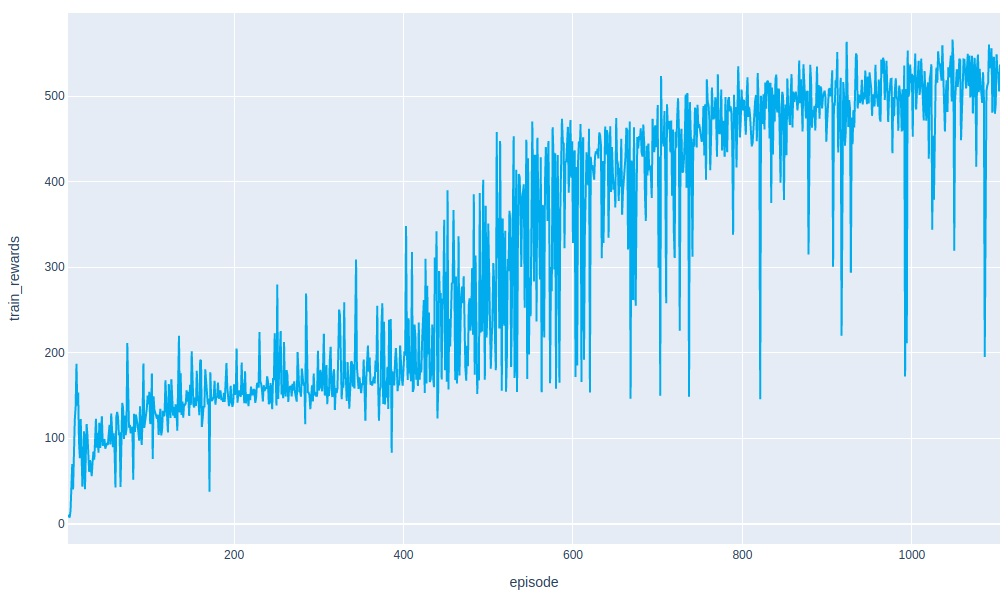
\includegraphics[width=1. \textwidth, height=.3\textheight]{pictures/train_resize}
\caption{ Performance obtained with the open source version of PlaNet at training time.}
\end{figure}

Like with the DDPG training, for every action, Gaussian noise is added, for this reason, there is a variance in the performance, but the training curve is monotonically increasing.

To find the real performance of the agent, we can see the test curve in which the same model is used without Gaussian noise.

\begin{figure}[H]
\centering
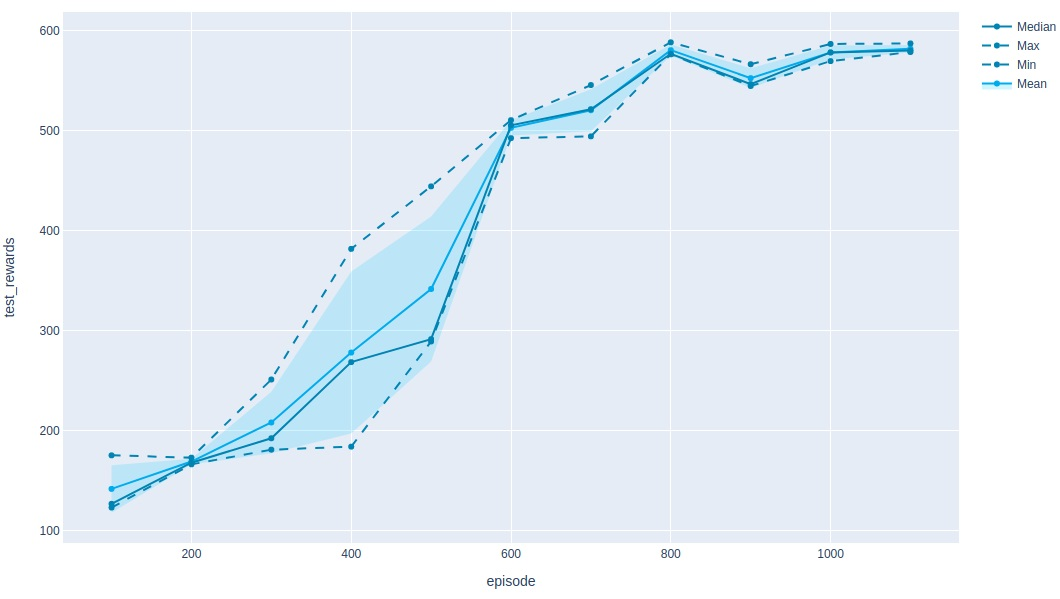
\includegraphics[width=1. \textwidth, height=.3\textheight]{pictures/test_resize}
\caption{ Performance obtained with the open source version of PlaNet at test time.}
\end{figure}

As we can see, after 1 million steps, the Planet agent is able to achieve a result of 578 rewards.


Beyond the final performances, it is interesting to deeply analyze the model predictions and the ability to generate predicted frames.
So in this experiment, we focus on the visual component of the prediction model.

We only provided the first frame to the model, and it predicted all the rest without receiving any further information beyond the actions performed at each step.

Both the observations and the predicted frames are resized to 64 x 64 pixels in order to reduce the computational cost. 

\begin{figure}[H]
\centering
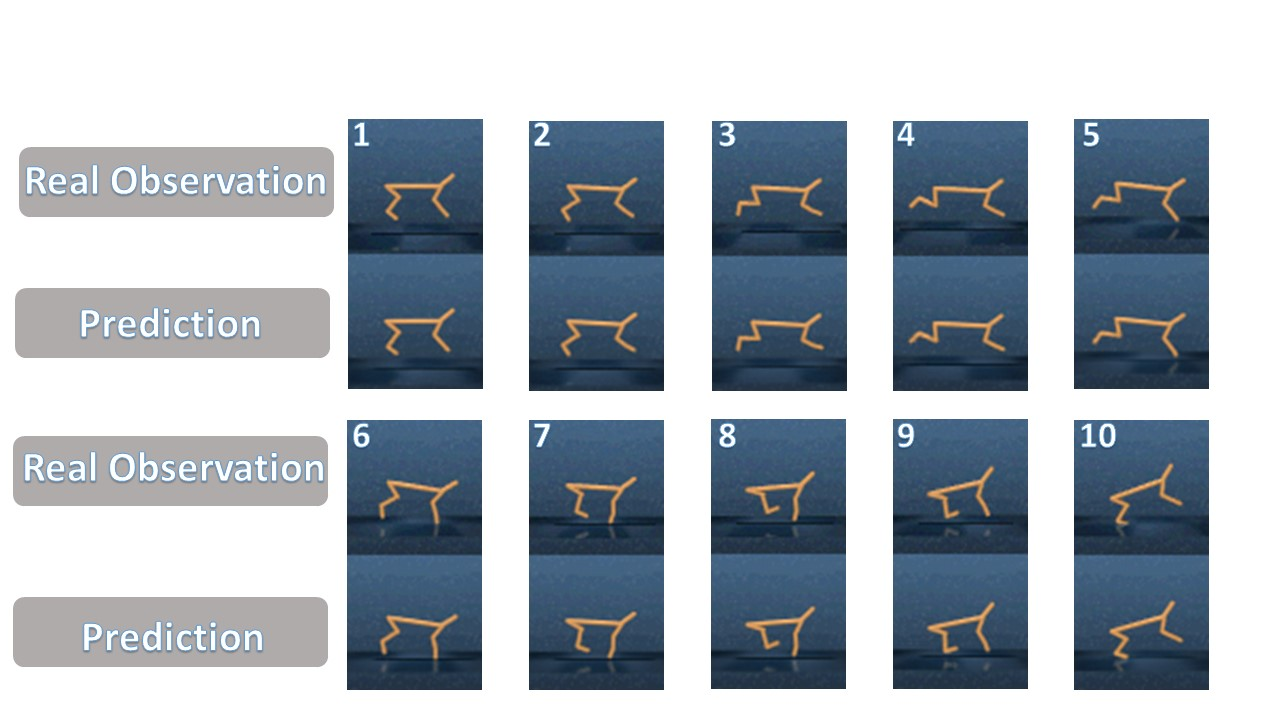
\includegraphics[width=1. \textwidth, height=.35\textheight]{pictures/dump_plan_init}
\caption{ Comparison between the first 10 real observations (the top frame) and the 10 predictions (the bottom frame).}
\end{figure}

As we can see from the image above, the model is able to predict all the first 10 steps correctly, but it is hard to keep the memory of the past experience for a long time, so as the predictions go on, the errors pile up.
Initially, these errors are barely perceptible. For this reason, we have extended the planning horizon up to 20 steps reaching the point where these errors are easily visible.

\begin{figure}[H]
\centering
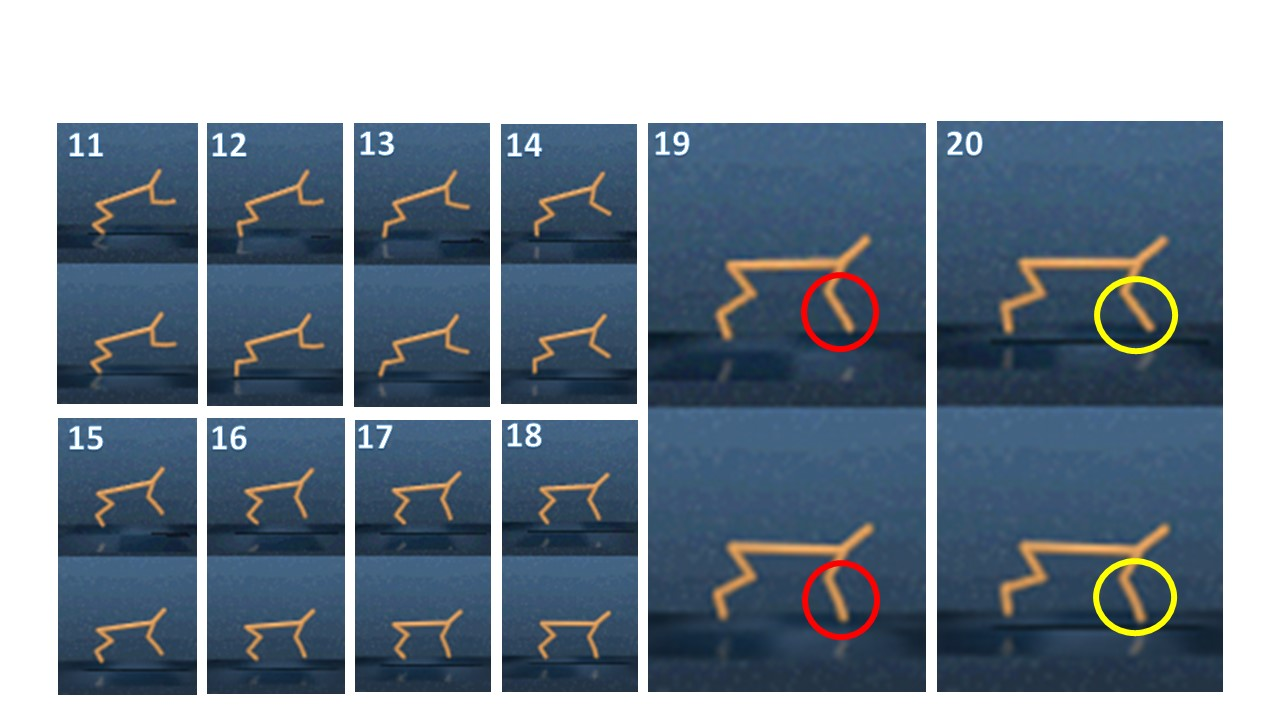
\includegraphics[width=1. \textwidth, height=.35\textheight]{pictures/dump_plan_finish}
\caption{ We can start to see discrepancies as the predictions goes on.}
\end{figure}

In order to make this comparison more clearly, we calculate the mean squared error (MSE) of each frames and we plot the pixels difference over the 20 planned steps.

\begin{figure}[H]
\centering
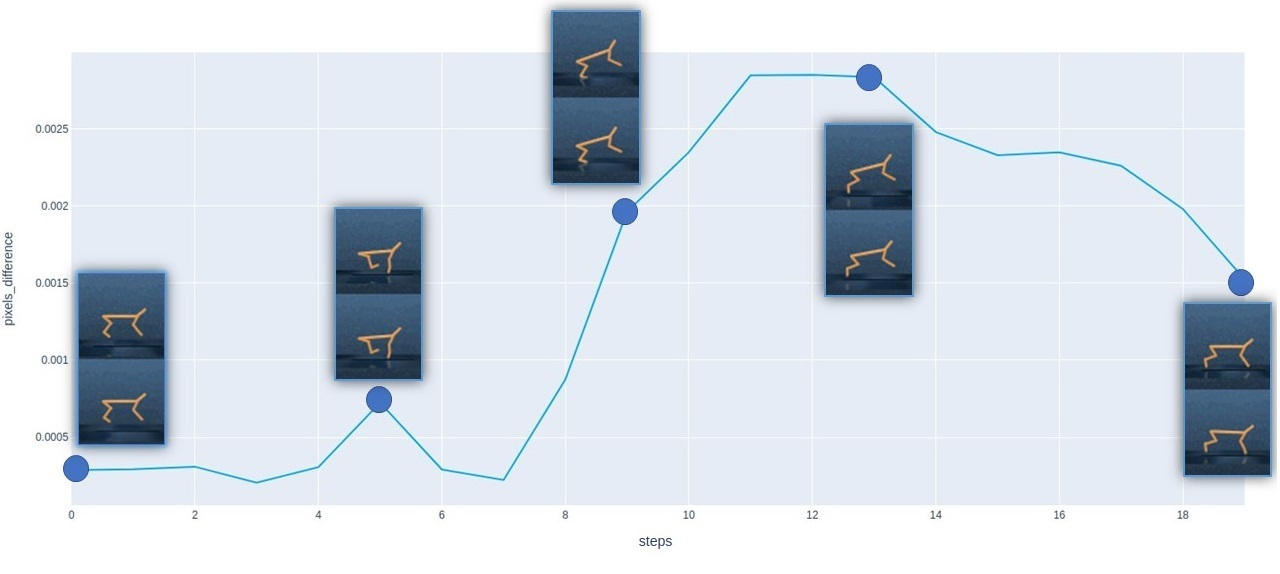
\includegraphics[width=1. \textwidth, height=.35\textheight]{pictures/pixels_difference}
\caption{The mean squared error of the real and predicted frames over 20 steps.}
\end{figure}
This is not a problem for the planning algorithm since the model predict only for a short horizon. In particular the authors of PlaNet has chosen a planning horizon of 12 steps.

We have also produced a heatmap to highlight the area in which the model produce the most errors.

\begin{figure}[H]
\centering
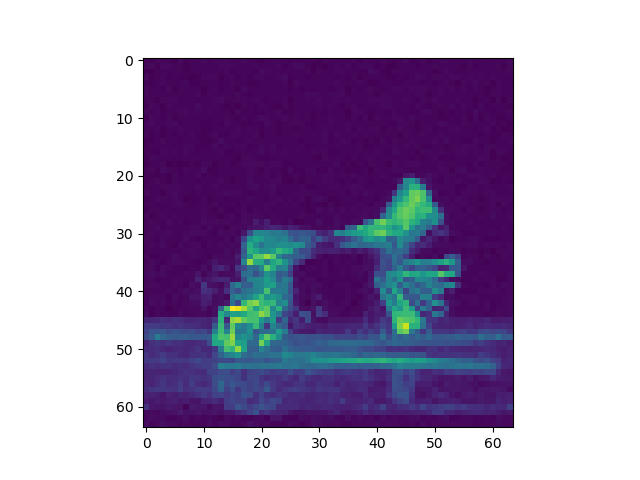
\includegraphics[width=1. \textwidth, height=.45\textheight]{pictures/heatmap}
\caption{The heatmap highlight the area of all the predicted frames where the model has made the greatest errors.}
\end{figure}
As we could expect the heatmap show that the model make more error in the area of the in the hind and front legs of the cheetah and in the zone of the head.

We also tested the reward predictions. The plot below show how close are the predictions of the fully trained model and the effective received reward for an entire episode.

\begin{figure}[H]
\centering
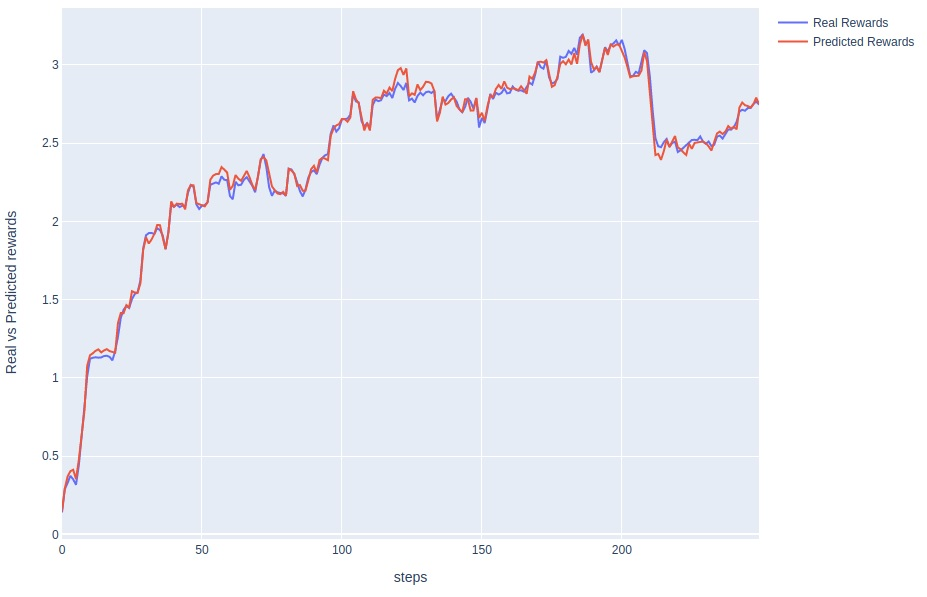
\includegraphics[width=1. \textwidth, height=.4\textheight]{pictures/rew_vs_pred_rew}
\caption{ Comparison between the reward model predictions and the effective reward obtained.}
\end{figure}


\section{Experiments with PlaNet}

In this section we investigate the chance to improve the performance of the open-source version of PlaNet. We tried three different ways.

The first try is about the preprocessing phase of each frame steps.
At each steps, the generated frame is preprocessed before being used as input to the model. In particular, operation of resizing is applied by the cv2 library using the INTER LINEAR algorithm.
Exploring the DeepMind Control Suite code, we saw that this process could be avoided indicating directly to the camera the size of the frame to be rendered with the command:
\textit{\texttt{self.\textunderscore env.physics.render(height=64, width=64, camera\textunderscore id=0)}}.
We found that also the original implementation uses a resize method instead of native render in low dimensions. In particular they use the \textit{"skimage.transform.resize"} method as you can see in \href{https://github.com/google-research/planet/blob/master/planet/control/wrappers.py}{their implementation}. 

We can see how changing this single one line of code has a huge positive impact on the final performance.

\begin{figure}[H]
\centering
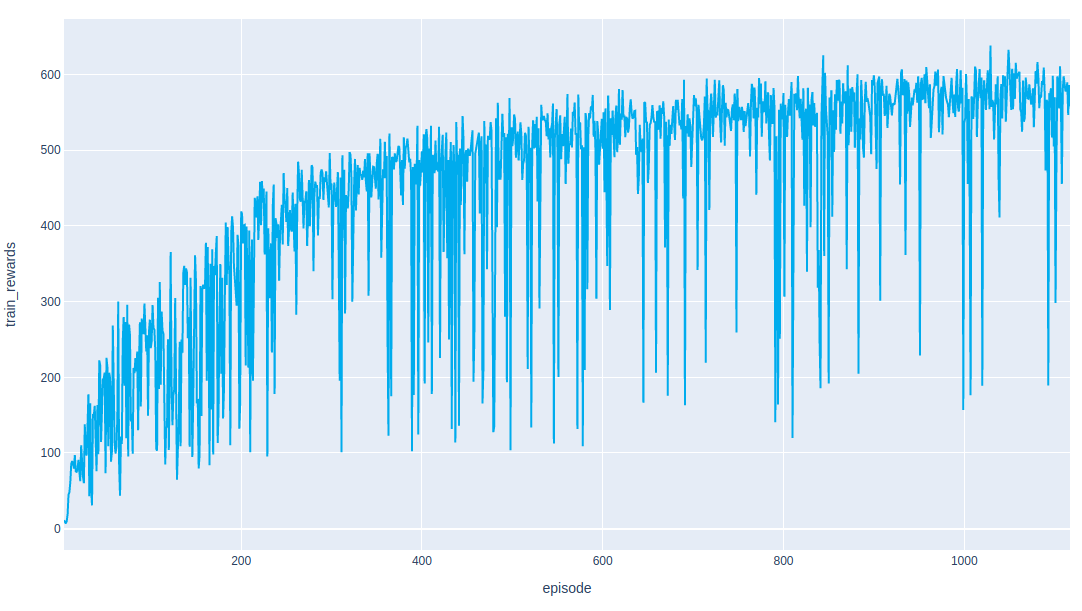
\includegraphics[width=1. \textwidth, height=.3\textheight]{pictures/train_planet_puro}
\caption{ Performance obtained at training time without resize the frames.}
\end{figure}

\begin{figure}[H]
\centering
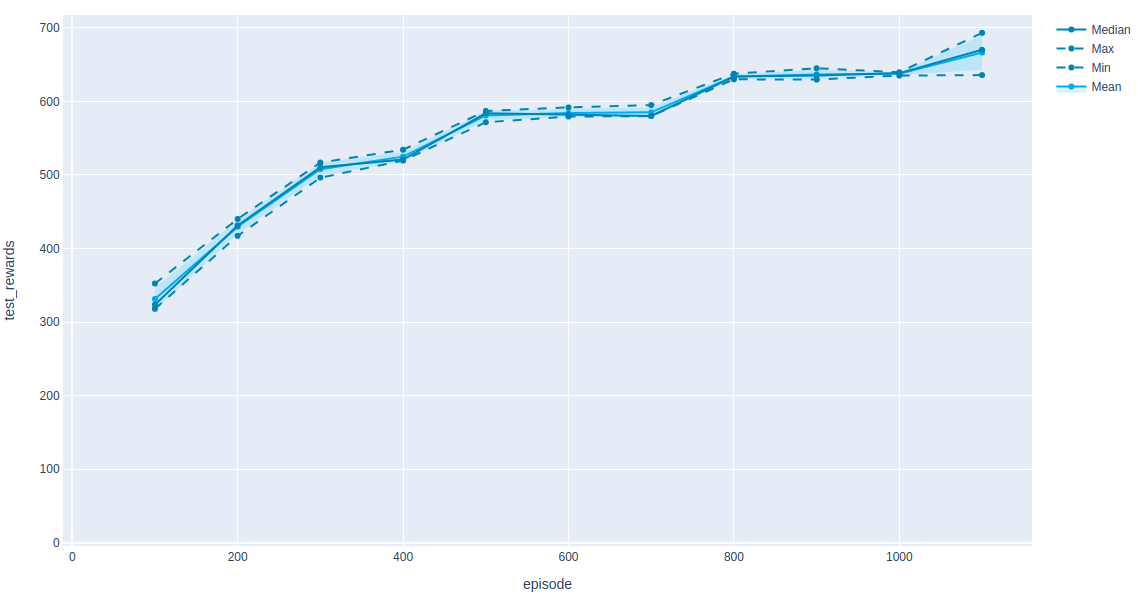
\includegraphics[width=1. \textwidth, height=.3\textheight]{pictures/test_planet_puro}
\caption{ Performance obtained at test time without resize the frame.}
\end{figure}

\begin{figure}[H]
\centering
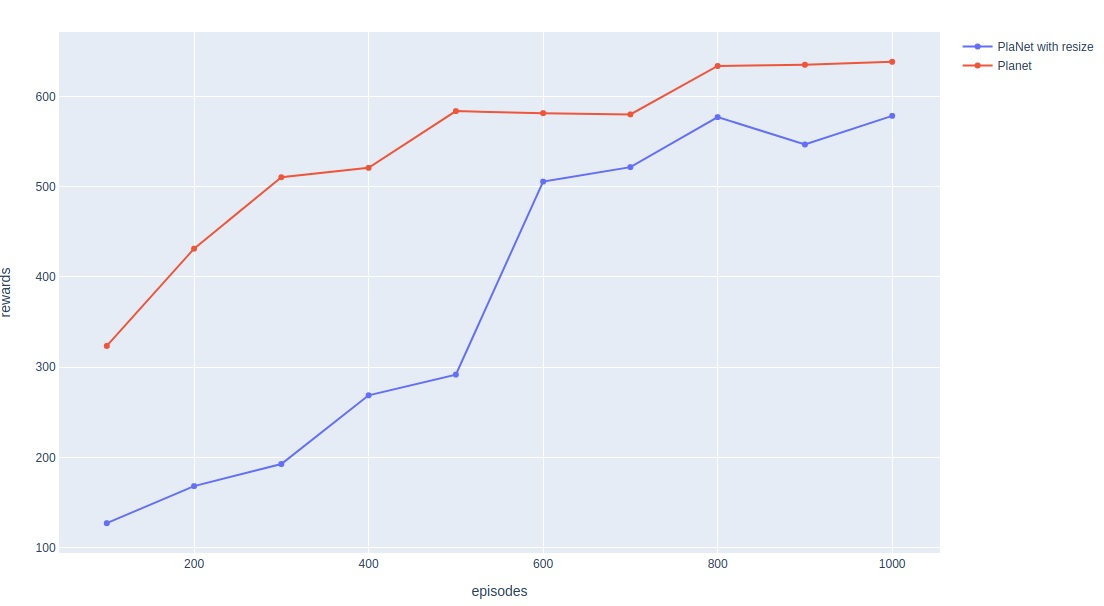
\includegraphics[width=1. \textwidth, height=.3\textheight]{pictures/resize_vs_pure}
\caption{ Comparison between the performance of PlaNet with and without the frames resizing.}
\end{figure}

We think that this improvement is due to the fact that some information is lost when the algorithm of resizing are applied in the preprocessing phase.
\\
A second experiment is based on the idea of enriching the information at each step with the obtained reward, in addition to the current frame. During the experiments, we notice that when the model is not fully trained can happen that it keeps doing the same action believing to collect rewards. Indeed what really happening is that the agent keeps predicting a reward when in the real environment, it doesn't receive any good feedback.
After some training iterations, the agent fits better the environment dynamics, and the problem disappears. So the idea is to explicitly provide also the received reward so the agent can use it to recognize, at inference time, that it's predictions are not consistent with what is really happening. So, we modify the model by concatenating the encoded current observation with the previous reward.

\begin{figure}[H]
\centering
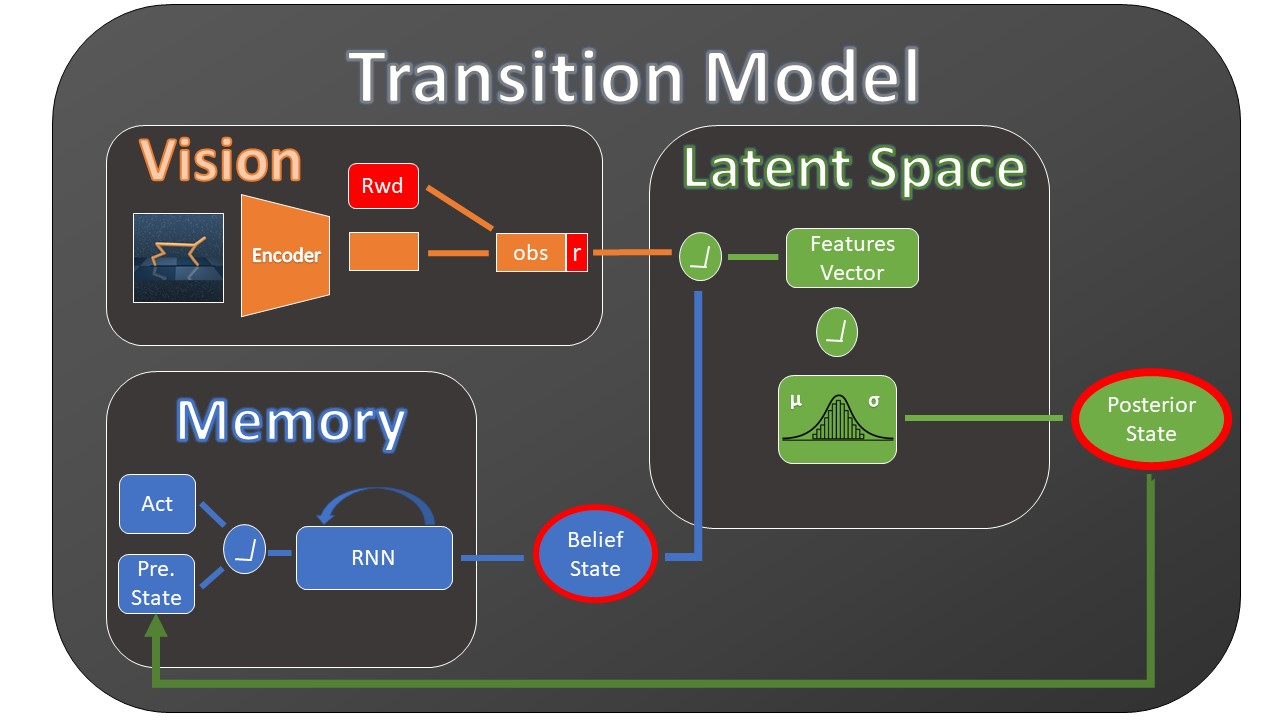
\includegraphics[width=1. \textwidth, height=.35\textheight]{pictures/planet_pred_as_rew}
\caption{ Concatenating the reward to the current observation.}
\end{figure}
The result of training seems to be not so promising. The training curve has more variance and does not overcome the previous version. 

\begin{figure}[H]
\centering
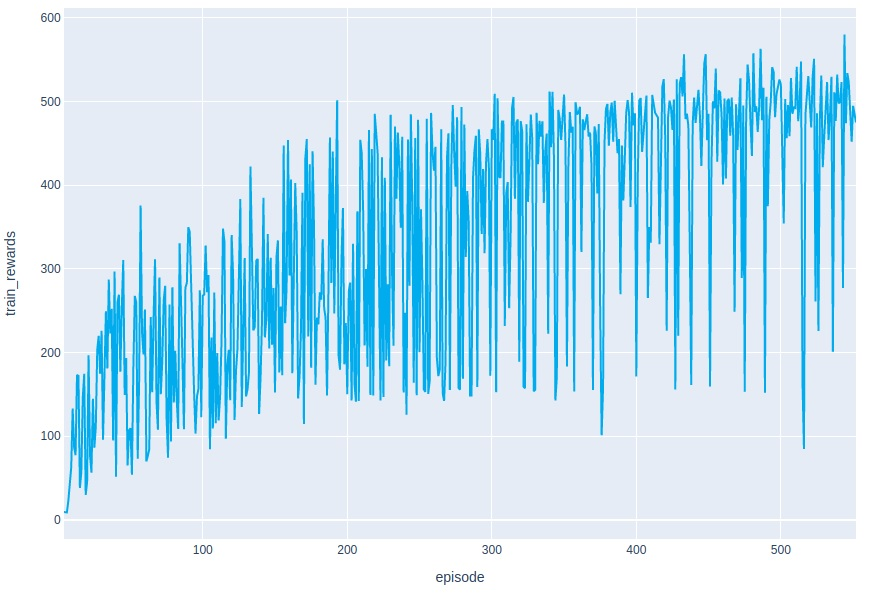
\includegraphics[width=1. \textwidth, height=.4\textheight]{pictures/planet_train_rew_as_state}
\caption{ Training curve of Planet model with reward as input.}
\end{figure}
The test curve confirms that this model is worse than the original. 

\begin{figure}[H]
\centering
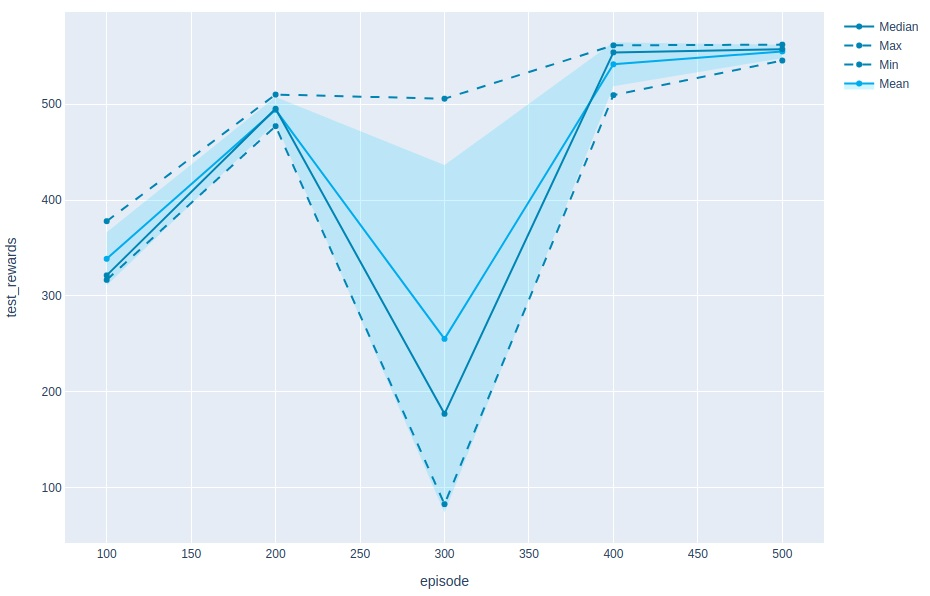
\includegraphics[width=1. \textwidth, height=.35\textheight]{pictures/planet_test_rew_as_state}
\caption{ The test curve is more unstable and achieve less cumulative reward than the original model. }
\end{figure}

After 500 iterations, we saw that the model is not outperforming the original version and we stop the experiment.

\begin{figure}[H]
\centering
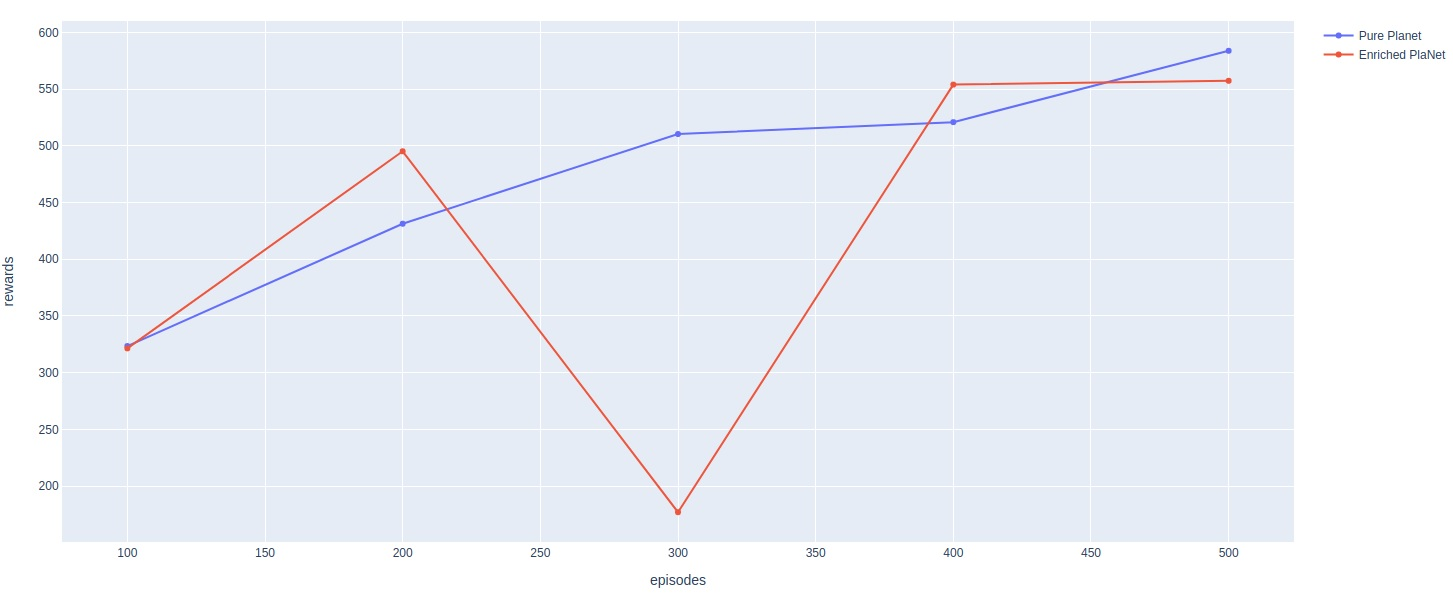
\includegraphics[width=1. \textwidth, height=.35\textheight]{pictures/rew_as_state_vs_pure_planet}
\caption{ The test curve is more unstable and achieve less cumulative reward than the original model. }
\end{figure}
We tried to add the reward information to other components of the model (e.g., in the memory module or directly in the reward module), but none of these tests worked and the presented version is the one that has given the best results. 
\\
The last idea is to add regularizer to improve the model predictions.
One of the main problems of using a planner in a model that is just an approximation of the real environment dynamics, is that the planner will exploit the learned model models inaccuracies. So, in the areas in which the model is uncertain, the predictions tend to be too optimistic and lead the planner to sub-optimal actions. 
We plot a comparison of the predicted and the rel reward obtained during the initial training episodes. From the image below we can see how initially the predictions tends to be too optimistic, and the provided plan fail to reach the expectations obtaining a low reward.

\begin{figure}[H]
\label{fig:original_rew_vs_pred}
\centering
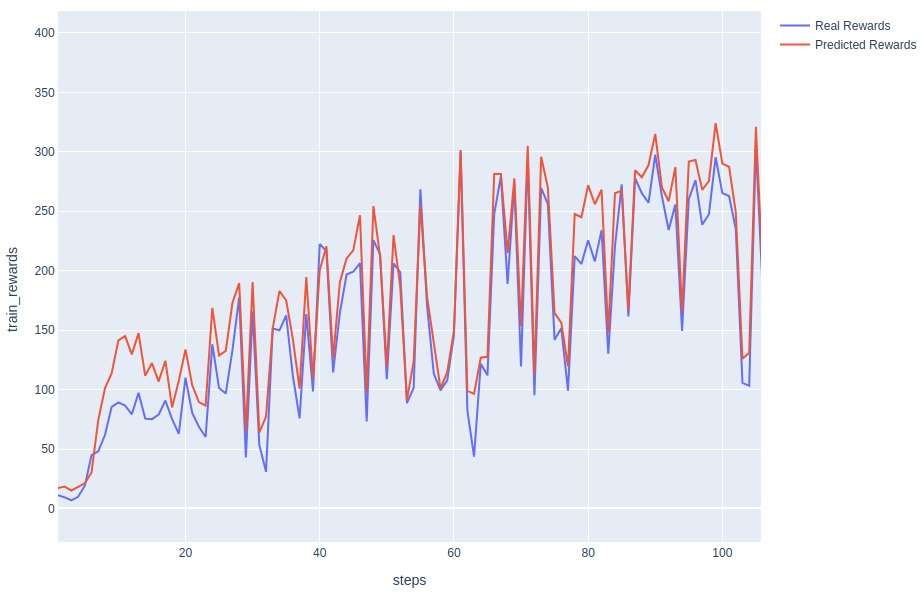
\includegraphics[width=1. \textwidth, height=.35\textheight]{pictures/original_pred_vs_real_rew}
\caption{ Comparison between the expected rewards predictions and the actual rewards obtained from the first 100 training episodes. }
\end{figure}
This problem is more severe in the early stages and less in later episodes when the agent has collected more data. Indeed, the more the agent interacts with the environment, the more data it collects, the more the predictions are precise. We are investigating a method to reduce this prediction gap just from the first episodes.

In their research, Rinu Boney et all \cite{boney2019regularizing} tries to alleviate this problem by penalizing the optimizer from considering trajectories that are outside the experience replay buffer ( that contains all the past experiences).
We call this new metric: \textbf{familiarity of the trajectories}.
So the planning objective is to maximize the rewards and also the familiarity of the plan respect to the data, with a new parameter $\alpha$ that modulates the weight between both costs.

$a_{t}^{*}, \ldots, a_{t+H}^{*}=\underset{a_{t}, \ldots, a_{t+H}}{\operatorname{argmax}} \sum_{\tau=t}^{t+H} r\left(s_{\tau}, a_{\tau}\right)+\alpha \log p\left(s_{t}, a_{t}, s_{t+1}, \ldots, s_{t+H}, a_{t+H}, s_{t+H+1}\right)$

Where $p(o_t, a_t, . . . , o_{t+H}, a_{t+H})$ is the probability of observing a given trajectory in the past experience.
They approximate the joint probability
of the whole trajectory as a sum of joint probabilities of each transition in the trajectory

$a_{t}^{*}, \ldots, a_{t+H}^{*}=\underset{a_{t}, \ldots, a_{t+H}}{\operatorname{argmax}} \sum_{\tau=t}^{t+H}\left[r\left(s_{\tau}, a_{\tau}\right)+\alpha \log p\left(s_{\tau}, a_{\tau}, s_{\tau+1}\right)\right]$

To calculate $\log p\left(s_{\tau}, a_{\tau}, s_{\tau+1}\right)$ they uses a denoising autoencoder (DAE).
DAE does not build an explicit probabilistic model $p\left(s_{\tau}, a_{\tau}, s_{\tau+1}\right)$ but learns to approximate the derivative of the log probability density.
To be more specific the theory of denoising states that, for zero-mean Gaussian corruption, the optima denoising function $g(\tilde{x})$ is given by:
$g(\tilde{x})=\tilde{x}+\sigma_{n}^{2} \frac{\partial}{\partial \tilde{x}} \log p(\tilde{x})$
where $\tilde{x}$  is the corrupted input, $p(\tilde{x})$ is the probability density function for $\tilde{x}$, $\sigma_n$ is the standard deviation of the Gaussian corruption.
So given the corrupted input $\tilde{x}$ and a fully trained DAE $g(\tilde{x})$, we can derive the gradient of the log-probability of the data distribution convolved with a Gaussian distribution:
$\frac{\partial}{\partial \tilde{x}} \log p(\tilde{x}) \propto g(x)-x$. 
They use $\frac{\partial}{\partial \tilde{x}} \log p(\tilde{x}) $ instead of $\frac{\partial}{\partial \tilde{x}} \log p(x) $ assuming $\frac{\partial}{\partial \tilde{x}} \log p(\tilde{x}) \approx \frac{\partial}{\partial x} \log p(x)$.
\\
For the experiments, they used an environment with low dimensional input (features state) and so with another model based algorithm, called PETS \cite{chua2018deep}. 
We initially try to replicate their solution, but the difference between the two models and the overload due to the processing of the image (they worked only with features vectors, not with frames) make the model so slow to be useless. 
For this reason, we use the same idea, but we implement it differently. We work directly with the prediction model and not with the planned.  Another fundamental difference is that we work at training time and not at inference time.
The PlaNet prediction model does not produce directly a new observation but works only in a latent space. So it makes no sense to train DAE with the observations collected in the dataset. Instead, we train the DAE directly in latent space also at training time.
The second difference is about the input dimension.
We feed the DAE with the entire plan at each step, so we train it by concatenating all the transitions according to the planning horizon parameter.
We experiments to different ways to concatenate transitions:
\begin{enumerate}
\item Concatenation of triplets: every transition is composed by 3 elements: $(s_t,a_t,s_{t+1})$. But in the final concatenation, all the elements placed at the extremes will be repeated: $[ (s_0,a_0,s_1) , (s_1,a_1,s_2) ... (s_{10},a_{10},s_{11}),  (s_{11},a_{11},s_{12}) ]$
\item Concatenation as chain: we remove the repetitions: $[ (s_0,a_0,s_1,a_2,s_2 ... s_{10},a_{10},s_{11},a_{11},s_{12}) ]$
\end{enumerate}

\begin{figure}[H]
\centering
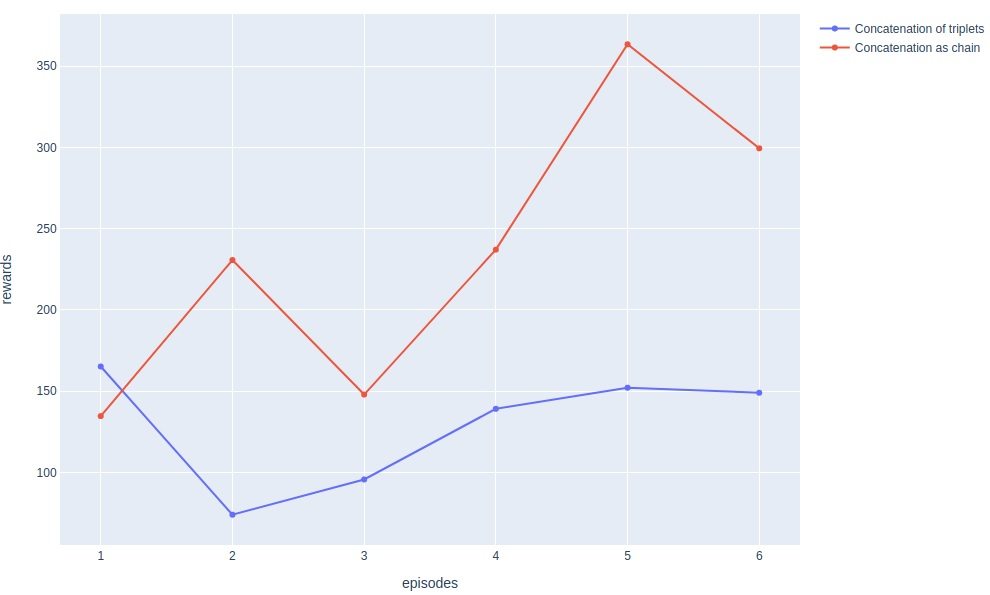
\includegraphics[width=.90 \textwidth, height=.25\textheight]{pictures/comparison_chain_vs_tripl}
\caption{ Comparison between the two strategies of input shape for the regularizer. }
\end{figure}

The final model architecture consists of one single linear layer with 600 units and a gaussian noise of zero mean and a standard deviation of 0.3.
The input dimension is the sum of the belief state size, the posterior state size, and the size of the actions multiplied for the planning horizon.
As we expected, the regularizer's effect is to improve the model predictions immediately and allow the model to increment the sample efficiently just from the initial episodes.


\begin{figure}[H]
\centering
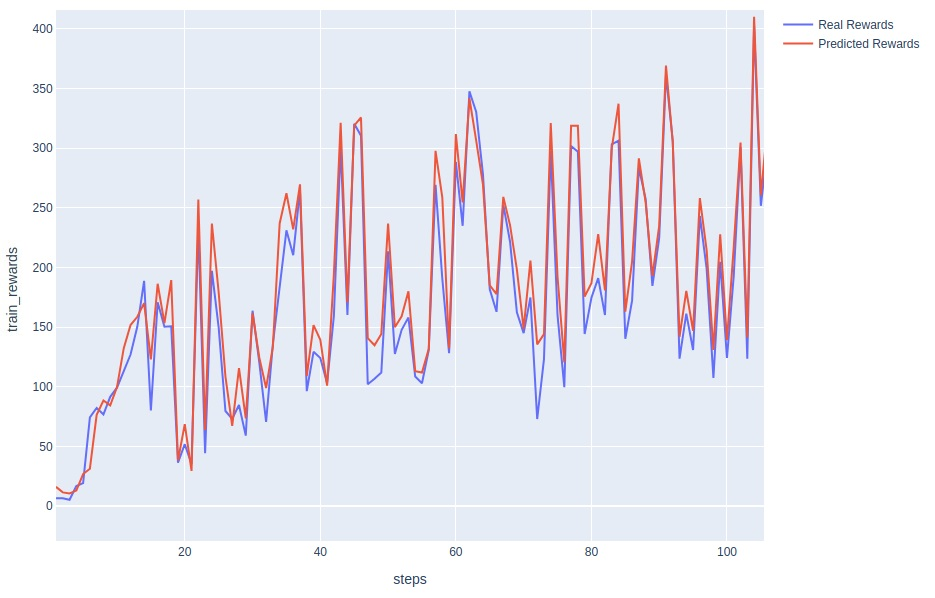
\includegraphics[width=1. \textwidth, height=.35\textheight]{pictures/reg_pred_vs_real_rew}
\caption{ Comparison between the expected rewards predictions and the actual rewards obtained from the first 100 training episodes with regularizer. }
\end{figure}
We can see from the image above that the reward's predictions start immediately to match with the real reward when the regularizer is activated.  
To make more clear the comparison between the prediction of the model with and without the regularizer, we created a new plot. 
In this plot we indicate the difference between the predicted reward and the obtained one over the episodes of the training. 
We can clearly see that the prediction error of the regularized model, represented with the blue line, is clearly lower in the initial episodes and that after some episodes the two values starts to converge.

\begin{figure}[H]
\centering
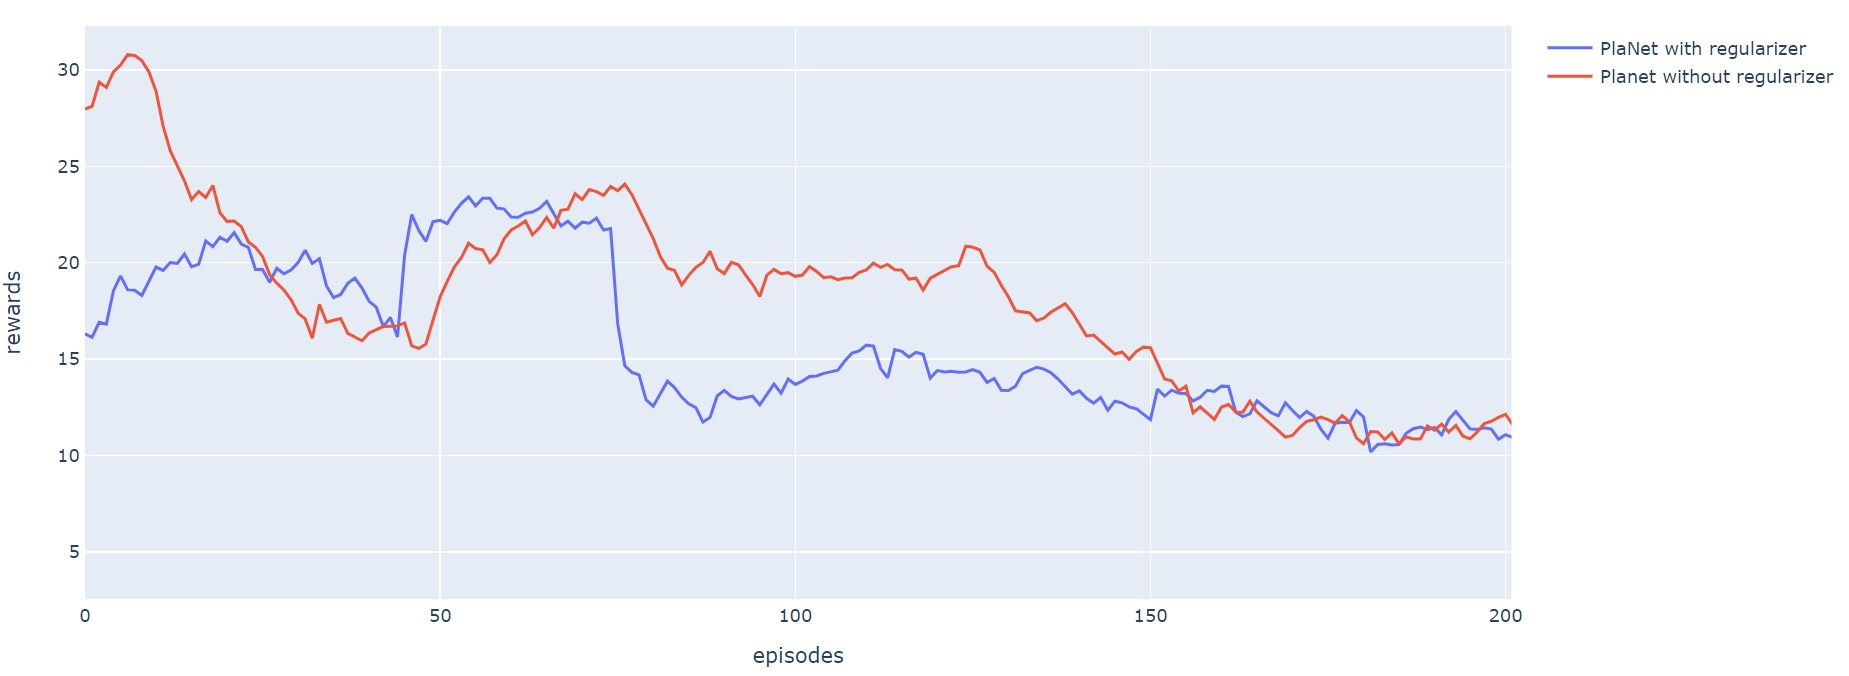
\includegraphics[width=1. \textwidth, height=.25\textheight]{pictures/plot_ass_diff}
\caption{ The absolute reward prediction error. The moving average technique is applied with a window of 30. }
\end{figure}

To be more clear we also calculate the relative error that remain consistent with the results above.

\begin{figure}[H]
\centering
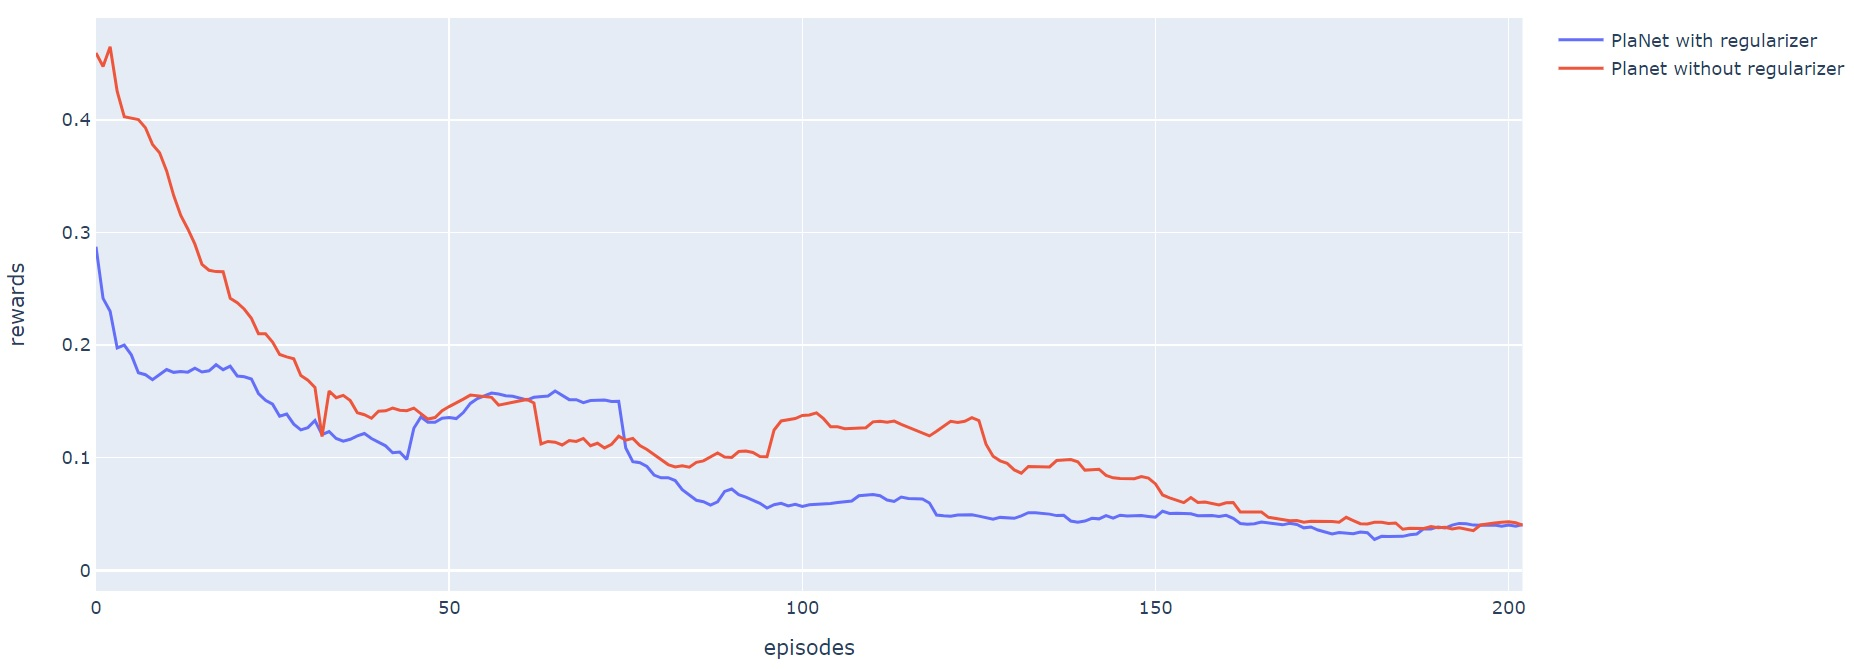
\includegraphics[width=1. \textwidth, height=.25\textheight]{pictures/plot_rel_diff}
\caption{ The relative reward prediction error. The moving average technique is applied with a window of 30. }
\end{figure}

This improvement allows the model to accumulate more rewards just in the initial episodes. This can be very useful where it is not possible to produce a huge amount of data.
\begin{figure}[H]
\centering
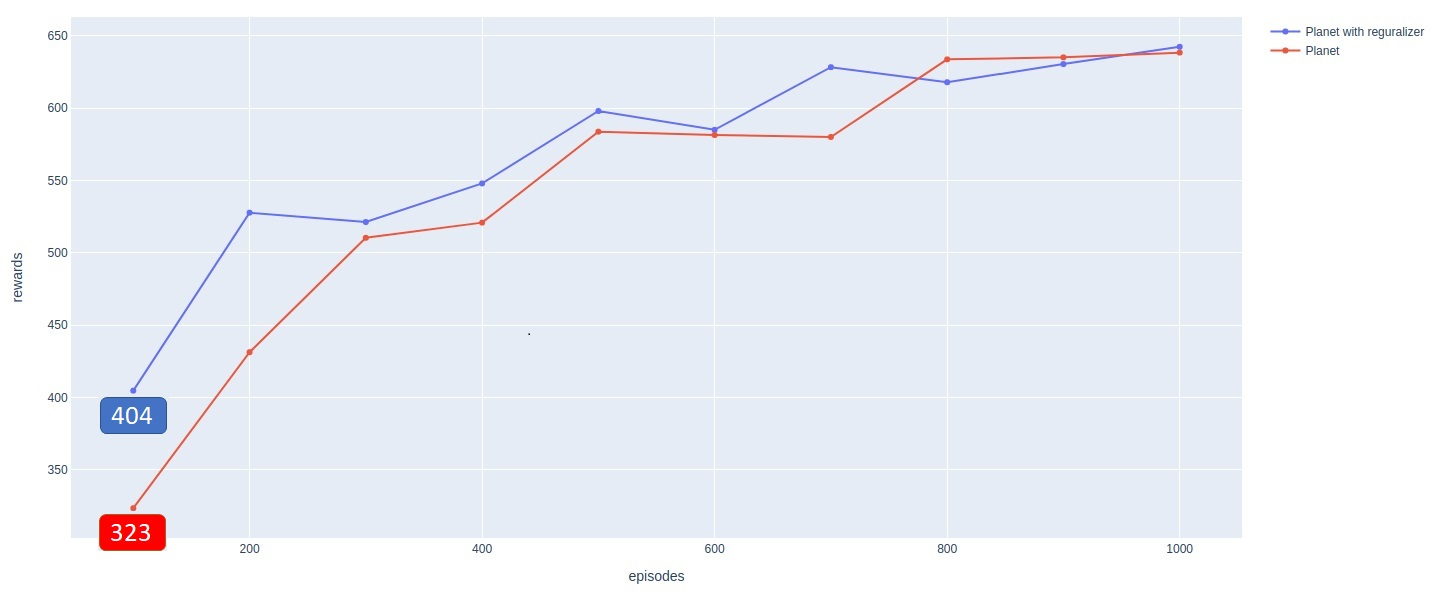
\includegraphics[width=1. \textwidth, height=.25\textheight]{pictures/full_reg_vs_original}
\caption{ Comparison between the full trained model with and without the regularizer.  }
\end{figure}

According to the research of Rinu Boney et all \cite{boney2019regularizing}, the improvement of the regularizer decrease during the training, but in our case, the performance of the original model does not surpass the performance of the model with regularized. 
%As suggested by the Rinu Boney et al. paper, "This result is evidence of the importance of exploration: the DAE regularization essentially penalizes exploration, which can harm asymptotic performance in complex environments."
We think that after a certain number of iterations, the model has accumulated enough knowledge about the environment to do without the regularizer. As proof of this, we point out that to achieve these results, we have to decrease the impact of the regularizer during training. From episode 750, we deactivate it entirely.
We observed an improvement, that needs to be validated with other experiments on other environments.


\section{Comparisons}
Now it's time to compare the model-based and the model-free approach. 

We specify that for this final comparison we use the DDPG result obtained with the model trained from the features vectors, while the PlaNet results are obtained with a model trained via raw pixels.

Despite the difference in the input complexity, the model-based approach achieves better results. In particular, in the initial phase, when the model has less sample and the regularizer influence is more intense.

\begin{figure}[H]
\centering
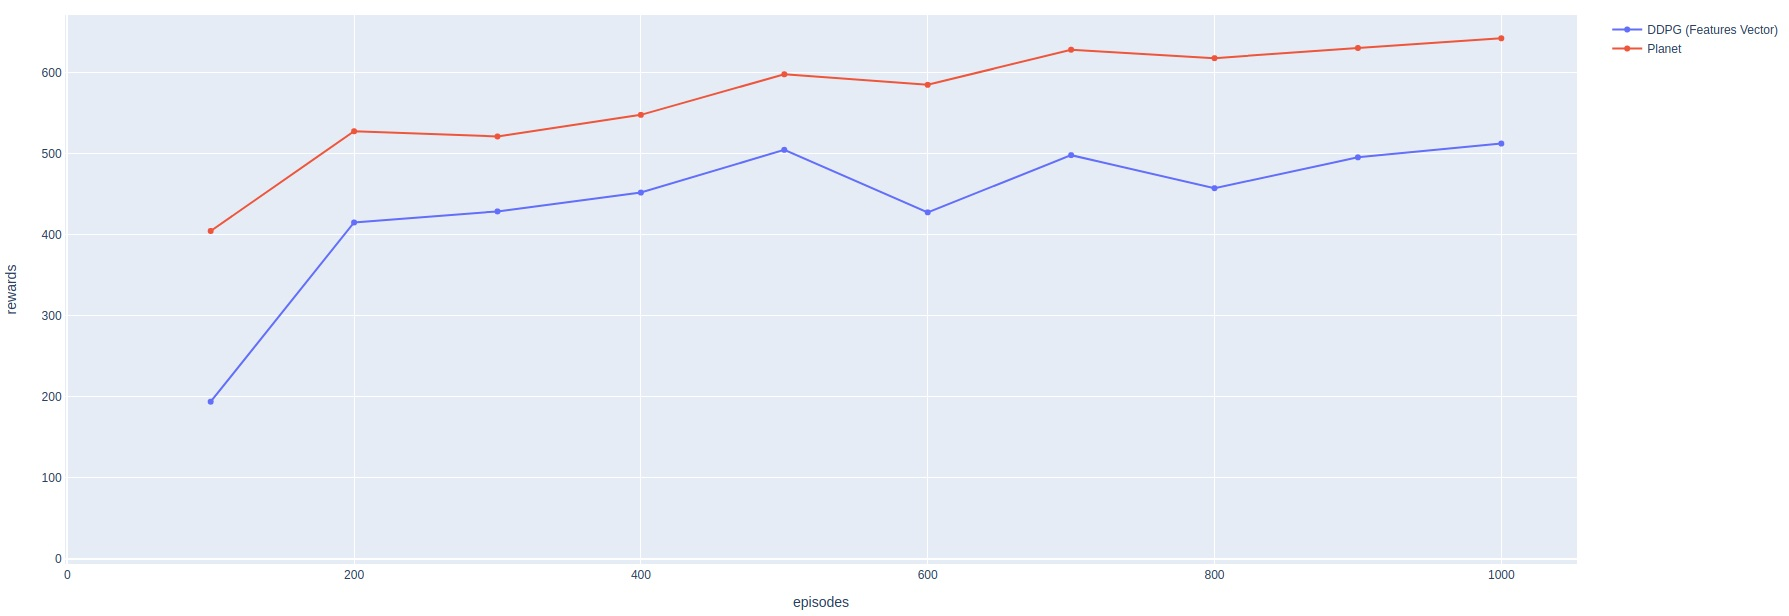
\includegraphics[width=1 \textwidth, height=.25\textheight]{pictures/ceetah_planet_vs_ddpg}
\caption{ Comparison between the performance of PlaNet (trained from frames) and DDPG (trained fro features vectors) for the Ceetah environment.  }
\end{figure}

We also tried other different environments, and we saw that PlaNet roughly maintain the advantage over DDPG. 
We specify that for these other environments, we do not use the regularizer.

\begin{figure}[H]
\centering
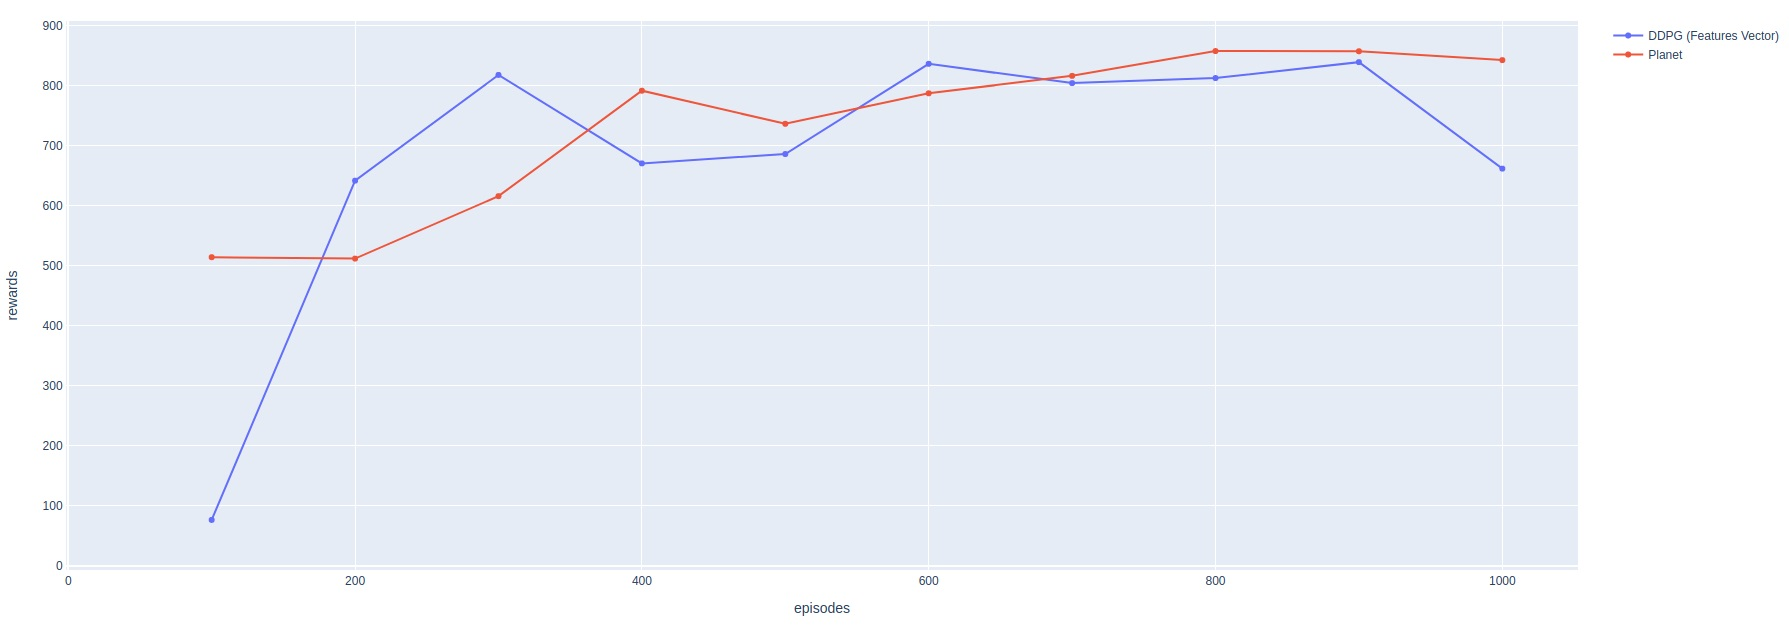
\includegraphics[width=1 \textwidth, height=.25\textheight]{pictures/cartpole_planet_vs_ddpg}
\caption{ Comparison between the performance of PlaNet (trained from frames) and DDPG (trained fro features vectors) for the Cartpole-Swingup environment.  }
\end{figure}
\begin{figure}[H]
\centering
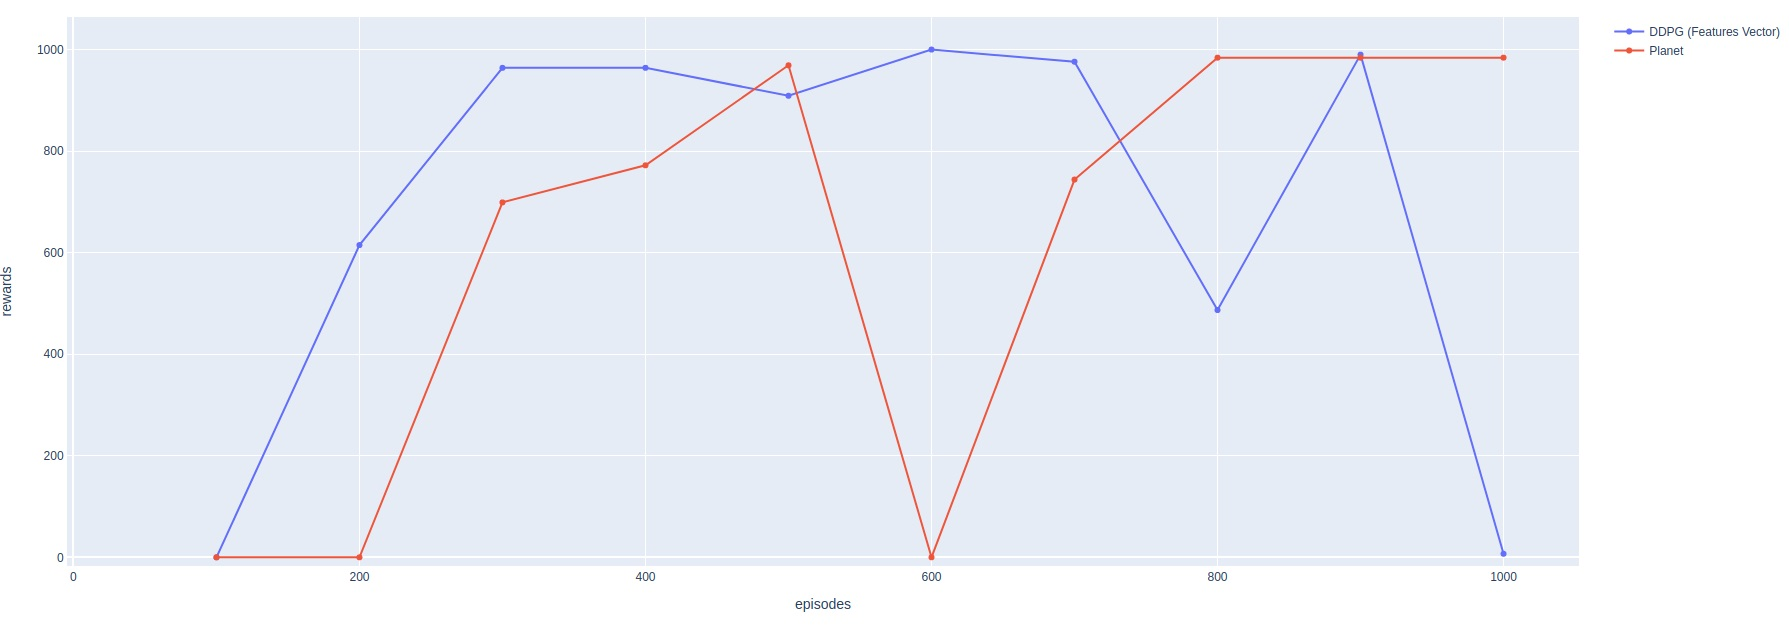
\includegraphics[width=1 \textwidth, height=.25\textheight]{pictures/reacher_planet_vs_ddpg}
\caption{ Comparison between the performance of PlaNet (trained from frames) and DDPG (trained fro features vectors) for the Reacher-easy environment.  }
\end{figure}
\begin{figure}[H]
\centering
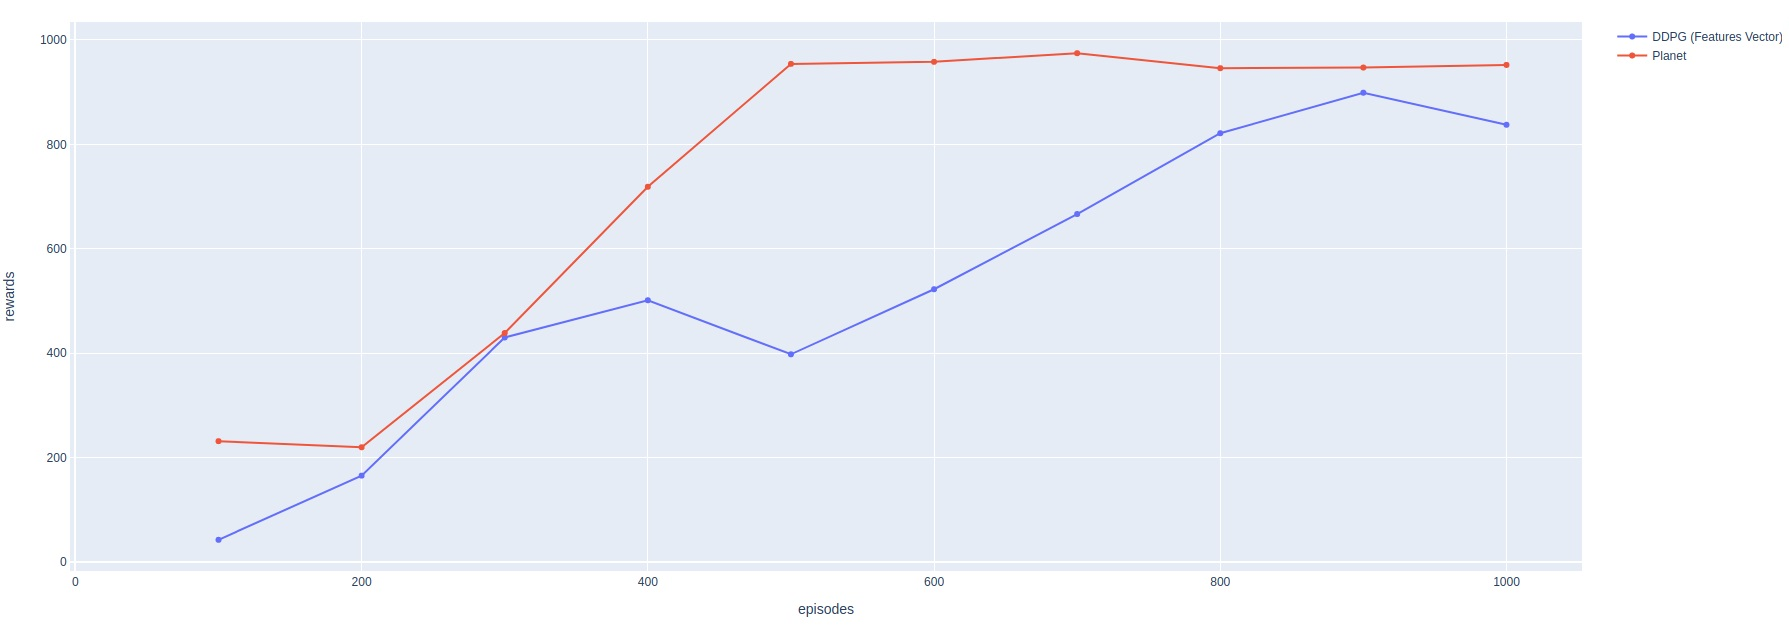
\includegraphics[width=1 \textwidth, height=.25\textheight]{pictures/walker_planet_vs_ddpg}
\caption{ Comparison between the performance of PlaNet (trained from frames) and DDPG (trained fro features vectors) for the Walker-walk environment.  }
\end{figure}

Coherently with the theory, we notice an evident difference between the training time for the model-based and model-free algorithm.
The PlaNet model can achieve a better result with less sample because it makes more calculations for each step. For this reason, the training time is longer when we train a model-based agent (the same is for the amount of GPU memory). Since the model-free has not a planner, it is also faster at inference time. 

\begin{figure}[H]
\centering
\includegraphics[width=1 \textwidth, height=.35 \textheight]{pictures/tempi_di_training}
\caption{ The plot shows a comparison between the training clock time (hours) required to train a DDPG linear model, DDPG convolutional model, PlaNet model and PlaNet model with the regularizer on a GPU Nvidia GeForce 1080ti..  }
\end{figure}
\clearemptydoublepage
% Chapter 7

\chapter{Conclusions} % Main chapter title

\label{Chapter7} % For referencing the chapter elsewhere, use \ref{Chapter1} 

This thesis aimed to make a comparison between the model-based and the model-free approach in the context of Deep Reinforcement Learning (DRL). A set of tests have been executed over four environments from DeepMind Control Suite. The DRL algorithm known as Deep Deterministic Policy Gradient is used to test the model-free approach, while the chosen model-based algorithm was PlaNet.

The DDPG algorithm was implemented and tested over all the four environments chosen for the experiments. Some modifications, suggested by the Control Suite authors, were applied to the original algorithm and  parameters to adapt them to the Control Suite environments. After this improvement, the algorithm has been able to learn a policy when a state feature was provided.
These suggestions are not provided for the version with raw-pixels input. This problem is more difficult since the input is way more complicated. Features state is described by a vector of 18 dimensions (for the cheetah problem) while a single frame is a 64x64 RGB image. For the raw pixels input version the Control Suite authors have used a more advanced version of the algorithm called Distributed Distributional Deterministic Policy Gradients (D4PG). They showed that this version could also learn in this condition but is not capable of achieving the same performances of the experiments with features vector as input.
Moreover, that model has required $10^8$ number of samples. For our work, we still tried to train a DDPG model with frames as input, but we have been not enough computational budget to reach such a high number of steps, so we stop the training after 1000 episodes ($10^6$ steps, like all the other experiments). These results showed how difficult is the problem of solving that benchmark environment directly from raw-pixels input. 

PlaNet algorithm instead is natively designed to work with raw-pixels, and so  the algorithm converged for all the tested environments. We also discovered how to improve the general performance by removing the frame's compression in the preprocessing phase asking directly the Control Suite to render the frames in the specific dimensions required.

Next, two main ideas to improve the PlaNet model were tested. The first one was about to use the obtained reward as additional information to enrich the current state, but it failed.
The second idea is based on the fact that the model performances are directly connected to the reward predictions. In the early episodes, where the model is not trained, it tends to be too optimistic and to give erroneous information to the planner. This leads to a suboptimal plan and so a low cumulated reward, because the planner will exploit the weaknesses of the predictive model instead of optimizing the real agent's behaviour. For this reason, the second idea was to improve the model prediction ability by forcing the predictions to stay close to the collected experience. In other words, during the training, we incremented the model loss when the prediction was "unlikely" with respect to the trajectory collected in the experience replay buffer. The persistence of the regularizer can penalize the model because it limits the exploration of the environment, so we reduce the impact of the it during the training. In this way, we obtained a positive impact from the first iterations, and we maintained the same performance in the last episodes. We see a positive impact from the use of the regularizer, and we believe it deserves further study and experimentation, even with other environments.

The PlaNet model was able to reach better results with respect to the DDPG algorithm even if it worked directly with raw pixels while DDPG worked with feature states. This result is confirmed also for the other three environments and showed how the model-based approach leads to better performance and more sample efficiency. Since the network architecture in the model-based approach is more complex, the training time is longer. The DDPG model is faster at inference time and required less clock time to be trained (but more samples). For the task of the train an agent in the real world, the sample efficiency is a critic parameter. In facts, the cost of acquiring samples in a real environment is an order of magnitude greater than train the model with them.
Furthermore, the RGB camera is a very common, powerful and generic (not single task-specific) type of sensor that a lot of real-world robots could use. For these reasons, even if PlaNet algorithm has not already tested in a real-world scenario, we consider it a fundamental milestone to achieve the use of the Reinforcement Learning for a robot in the real world.

The following could be possible improvements for future research directions.\\

DDPG works well when a full markovian state is provided. We saw that the PlaNet model could produce a latent space that contains enough information to allow predictions over multiple steps. An interesting experiment could be to use PlaNet as an encoder to produce the latent states used then to train the DDPG algorithm. \\
%dreamer: https://arxiv.org/pdf/1912.01603.pdf

In the model-based approach, the planner ability is fixed and does not improve during the training epochs, as we saw with the model-free policy. The performance improvements are due to the increment of the knowledge about the environment that allows the model to make better predictions. So, to have a better model, we need to reduce the uncertainty over the environment. An idea of improvement could be the change of the planner objective in favour of the exploration during training. Once the model is fully trained a reward exploiting objective could be restored.
%plan to explore: https://arxiv.org/pdf/2005.05960.pdf


\clearemptydoublepage




%%%% TAIL OF THE DOCUMENT
\backmatter
%list of figures
\listoffigures
\clearemptydoublepage
\clearemptydoublepage
%bibliography
\addcontentsline{toc}{chapter}{Bibliography}
\bibliography{bibliography/bibThesis}
\bibliographystyle{ieeetr}
\clearemptydoublepage


\end{document}
